\documentclass[journal,12pt,twocolumn]{IEEEtran}
%
\usepackage{setspace}
\usepackage{gensymb}
%\doublespacing
\singlespacing

%\usepackage{graphicx}
%\usepackage{amssymb}
%\usepackage{relsize}
\usepackage[cmex10]{amsmath}
%\usepackage{amsthm}
%\interdisplaylinepenalty=2500
%\savesymbol{iint}
%\usepackage{txfonts}
%\restoresymbol{TXF}{iint}
%\usepackage{wasysym}
\usepackage{amsthm}
\usepackage{iithtlc}
\usepackage{mathrsfs}
\usepackage{txfonts}
\usepackage{stfloats}
\usepackage{bm}
\usepackage{cite}
\usepackage{cases}
\usepackage{subfig}
%\usepackage{xtab}
\usepackage{longtable}
\usepackage{multirow}
%\usepackage{algorithm}
%\usepackage{algpseudocode}
\usepackage{enumitem}
\usepackage{mathtools}
\usepackage{tikz}
\usepackage{circuitikz}
\usepackage{verbatim}
\usepackage{tfrupee}
\usepackage[breaklinks=true]{hyperref}
%\usepackage{stmaryrd}
\usepackage{tkz-euclide} % loads  TikZ and tkz-base
\usetkzobj{all}
\usepackage{listings}
    \usepackage{color}                                            %%
    \usepackage{array}                                            %%
    \usepackage{longtable}                                        %%
    \usepackage{calc}                                             %%
    \usepackage{multirow}                                         %%
    \usepackage{hhline}                                           %%
    \usepackage{ifthen}                                           %%
  %optionally (for landscape tables embedded in another document): %%
    \usepackage{lscape}     
\usepackage{multicol}
\usepackage{chngcntr}
%\usepackage{enumerate}

%\usepackage{wasysym}
%\newcounter{MYtempeqncnt}
\DeclareMathOperator*{\Res}{Res}
%\renewcommand{\baselinestretch}{2}
\renewcommand\thesection{\arabic{section}}
\renewcommand\thesubsection{\thesection.\arabic{subsection}}
\renewcommand\thesubsubsection{\thesubsection.\arabic{subsubsection}}

\renewcommand\thesectiondis{\arabic{section}}
\renewcommand\thesubsectiondis{\thesectiondis.\arabic{subsection}}
\renewcommand\thesubsubsectiondis{\thesubsectiondis.\arabic{subsubsection}}

% correct bad hyphenation here
\hyphenation{op-tical net-works semi-conduc-tor}
\def\inputGnumericTable{}                                 %%

\lstset{
%language=C,
frame=single, 
breaklines=true,
columns=fullflexible
}
%\lstset{
%language=tex,
%frame=single, 
%breaklines=true
%}

\begin{document}
%


\newtheorem{theorem}{Theorem}[section]
\newtheorem{problem}{Problem}
\newtheorem{proposition}{Proposition}[section]
\newtheorem{lemma}{Lemma}[section]
\newtheorem{corollary}[theorem]{Corollary}
\newtheorem{example}{Example}[section]
\newtheorem{definition}[problem]{Definition}
%\newtheorem{thm}{Theorem}[section] 
%\newtheorem{defn}[thm]{Definition}
%\newtheorem{algorithm}{Algorithm}[section]
%\newtheorem{cor}{Corollary}
\newcommand{\BEQA}{\begin{eqnarray}}
\newcommand{\EEQA}{\end{eqnarray}}
\newcommand{\define}{\stackrel{\triangle}{=}}

\bibliographystyle{IEEEtran}
%\bibliographystyle{ieeetr}


\providecommand{\mbf}{\mathbf}
\providecommand{\pr}[1]{\ensuremath{\Pr\left(#1\right)}}
\providecommand{\qfunc}[1]{\ensuremath{Q\left(#1\right)}}
\providecommand{\sbrak}[1]{\ensuremath{{}\left[#1\right]}}
\providecommand{\lsbrak}[1]{\ensuremath{{}\left[#1\right.}}
\providecommand{\rsbrak}[1]{\ensuremath{{}\left.#1\right]}}
\providecommand{\brak}[1]{\ensuremath{\left(#1\right)}}
\providecommand{\lbrak}[1]{\ensuremath{\left(#1\right.}}
\providecommand{\rbrak}[1]{\ensuremath{\left.#1\right)}}
\providecommand{\cbrak}[1]{\ensuremath{\left\{#1\right\}}}
\providecommand{\lcbrak}[1]{\ensuremath{\left\{#1\right.}}
\providecommand{\rcbrak}[1]{\ensuremath{\left.#1\right\}}}
\theoremstyle{remark}
\newtheorem{rem}{Remark}
\newcommand{\sgn}{\mathop{\mathrm{sgn}}}
\providecommand{\abs}[1]{\left\vert#1\right\vert}
\providecommand{\res}[1]{\Res\displaylimits_{#1}} 
\providecommand{\norm}[1]{\left\lVert#1\right\rVert}
%\providecommand{\norm}[1]{\lVert#1\rVert}
\providecommand{\mtx}[1]{\mathbf{#1}}
\providecommand{\mean}[1]{E\left[ #1 \right]}
\providecommand{\fourier}{\overset{\mathcal{F}}{ \rightleftharpoons}}
%\providecommand{\hilbert}{\overset{\mathcal{H}}{ \rightleftharpoons}}
\providecommand{\system}{\overset{\mathcal{H}}{ \longleftrightarrow}}
	%\newcommand{\solution}[2]{\textbf{Solution:}{#1}}
\newcommand{\solution}{\noindent \textbf{Solution: }}
\newcommand{\cosec}{\,\text{cosec}\,}
\providecommand{\dec}[2]{\ensuremath{\overset{#1}{\underset{#2}{\gtrless}}}}
\newcommand{\myvec}[1]{\ensuremath{\begin{pmatrix}#1\end{pmatrix}}}
\newcommand{\mydet}[1]{\ensuremath{\begin{vmatrix}#1\end{vmatrix}}}
%\numberwithin{equation}{section}
\numberwithin{equation}{subsection}
%\numberwithin{problem}{section}
%\numberwithin{definition}{section}
\makeatletter
\@addtoreset{figure}{problem}
\makeatother

\let\StandardTheFigure\thefigure
\let\vec\mathbf
%\renewcommand{\thefigure}{\theproblem.\arabic{figure}}
\renewcommand{\thefigure}{\theproblem}
%\setlist[enumerate,1]{before=\renewcommand\theequation{\theenumi.\arabic{equation}}
%\counterwithin{equation}{enumi}


%\renewcommand{\theequation}{\arabic{subsection}.\arabic{equation}}

\def\putbox#1#2#3{\makebox[0in][l]{\makebox[#1][l]{}\raisebox{\baselineskip}[0in][0in]{\raisebox{#2}[0in][0in]{#3}}}}
     \def\rightbox#1{\makebox[0in][r]{#1}}
     \def\centbox#1{\makebox[0in]{#1}}
     \def\topbox#1{\raisebox{-\baselineskip}[0in][0in]{#1}}
     \def\midbox#1{\raisebox{-0.5\baselineskip}[0in][0in]{#1}}

\vspace{3cm}

\title{
	\logo{
Optimization through School Geometry
	}
}
\author{ G V V Sharma$^{*}$% <-this % stops a space
	\thanks{*The author is with the Department
		of Electrical Engineering, Indian Institute of Technology, Hyderabad
		502285 India e-mail:  gadepall@iith.ac.in. All content in this manual is released under GNU GPL.  Free and open source.}
	
}	
%\title{
%	\logo{Matrix Analysis through Octave}{\begin{center}\includegraphics[scale=.24]{tlc}\end{center}}{}{HAMDSP}
%}


% paper title
% can use linebreaks \\ within to get better formatting as desired
%\title{Matrix Analysis through Octave}
%
%
% author names and IEEE memberships
% note positions of commas and nonbreaking spaces ( ~ ) LaTeX will not break
% a structure at a ~ so this keeps an author's name from being broken across
% two lines.
% use \thanks{} to gain access to the first footnote area
% a separate \thanks must be used for each paragraph as LaTeX2e's \thanks
% was not built to handle multiple paragraphs
%

%\author{<-this % stops a space
%\thanks{}}
%}
% note the % following the last \IEEEmembership and also \thanks - 
% these prevent an unwanted space from occurring between the last author name
% and the end of the author line. i.e., if you had this:
% 
% \author{....lastname \thanks{...} \thanks{...} }
%                     ^------------^------------^----Do not want these spaces!
%
% a space would be appended to the last name and could cause every name on that
% line to be shifted left slightly. This is one of those "LaTeX things". For
% instance, "\textbf{A} \textbf{B}" will typeset as "A B" not "AB". To get
% "AB" then you have to do: "\textbf{A}\textbf{B}"
% \thanks is no different in this regard, so shield the last } of each \thanks
% that ends a line with a % and do not let a space in before the next \thanks.
% Spaces after \IEEEmembership other than the last one are OK (and needed) as
% you are supposed to have spaces between the names. For what it is worth,
% this is a minor point as most people would not even notice if the said evil
% space somehow managed to creep in.



% The paper headers
%\markboth{Journal of \LaTeX\ Class Files,~Vol.~6, No.~1, January~2007}%
%{Shell \MakeLowercase{\textit{et al.}}: Bare Demo of IEEEtran.cls for Journals}
% The only time the second header will appear is for the odd numbered pages
% after the title page when using the twoside option.
% 
% *** Note that you probably will NOT want to include the author's ***
% *** name in the headers of peer review papers.                   ***
% You can use \ifCLASSOPTIONpeerreview for conditional compilation here if
% you desire.




% If you want to put a publisher's ID mark on the page you can do it like
% this:
%\IEEEpubid{0000--0000/00\$00.00~\copyright~2007 IEEE}
% Remember, if you use this you must call \IEEEpubidadjcol in the second
% column for its text to clear the IEEEpubid mark.



% make the title area
\maketitle

\newpage

\tableofcontents

\bigskip

\renewcommand{\thefigure}{\theenumi}
\renewcommand{\thetable}{\theenumi}
%\renewcommand{\theequation}{\theenumi}

%\begin{abstract}
%%\boldmath
%In this letter, an algorithm for evaluating the exact analytical bit error rate  (BER)  for the piecewise linear (PL) combiner for  multiple relays is presented. Previous results were available only for upto three relays. The algorithm is unique in the sense that  the actual mathematical expressions, that are prohibitively large, need not be explicitly obtained. The diversity gain due to multiple relays is shown through plots of the analytical BER, well supported by simulations. 
%
%\end{abstract}
% IEEEtran.cls defaults to using nonbold math in the Abstract.
% This preserves the distinction between vectors and scalars. However,
% if the journal you are submitting to favors bold math in the abstract,
% then you can use LaTeX's standard command \boldmath at the very start
% of the abstract to achieve this. Many IEEE journals frown on math
% in the abstract anyway.

% Note that keywords are not normally used for peerreview papers.
%\begin{IEEEkeywords}
%Cooperative diversity, decode and forward, piecewise linear
%\end{IEEEkeywords}



% For peer review papers, you can put extra information on the cover
% page as needed:
% \ifCLASSOPTIONpeerreview
% \begin{center} \bfseries EDICS Category: 3-BBND \end{center}
% \fi
%
% For peerreview papers, this IEEEtran command inserts a page break and
% creates the second title. It will be ignored for other modes.
%\IEEEpeerreviewmaketitle

\begin{abstract}
This book provides an introduction to optimization  based on the NCERT textbooks from Class 6-12.  Links to sample Python codes are available in the text.  
\end{abstract}
Download python codes using 
\begin{lstlisting}
svn co https://github.com/gadepall/school/trunk/ncert/optimization/codes
\end{lstlisting}

%\section{Triangle}
%\subsection{Triangle Examples}
%\renewcommand{\theequation}{\theenumi}
\begin{enumerate}[label=\arabic*.,ref=\thesubsection.\theenumi]
\numberwithin{equation}{enumi}
%\item If three  sides of one triangle are equal to three sides  of the other triangle, then the two triangles are congruent (SSS Congruence Rule).
%%
%\\
%\solution Using cosine formula in \eqref{eq:b_cos_form}, it can be shown that the angles of the triangle are also equal, hnce they are congruent.
% 	
%\item If two sides and the included angle of one triangle are equal to two sides and the included angle of the other triangle, then the two triangles are congruent (SAS Congruence Rule).
%\\
%\solution Use cosine formula in \eqref{eq:b_cos_form}.
%\item  If two angles and the included side of one triangle are equal to two angles and the included side of the other triangle, then the two triangles are congruent (ASA Congruence Rule).
%%
%\\
%\solution  Use the sine formula in \eqref{eq:sin_form} to show that the corresponding sides opposite the angles are equal. 
%\item If two angles and one side of one triangle are equal to two angles and the corresponding side of the other triangle, then the two triangles are congruent (AAS Congruence Rule)
%\\
%\solution Use the sine formula in \eqref{eq:sin_form}

%\item  In a triangle, angle opposite to the longer side is larger (greater). 
%%
%\label{prob:tri_ang_side_greater}
%%
%\\
%\solution Consider a right triangle $ABC$ right angled at $B$ as in Fig. \ref{fig:tri_ang_side_greater}.  From Baudhayana's theorem, 
%%
%\begin{align}
%\label{eq:tri_ang_side_greater_baudhb}
%b^2 &= a^2+c^2
%\\
%p^2 &= a^2+x^2
%\label{eq:tri_ang_side_greater_baudhp}
%\end{align}
%%
%$\because c > x$, from \eqref{eq:tri_ang_side_greater_baudhb} and \eqref{eq:tri_ang_side_greater_baudhp}, is obvious that %
%\begin{align}
%\label{eq:tri_ang_side_greater_baudhbp}
%b > p \implies \frac{b}{p} > 1
%\end{align}
%%
%Also, from \eqref{eq:sin_form_def},
%%
%%
%\begin{align}
%%\label{eq:tri_ang_side_greater_baudh_bp}
%a = b\sin A &= p \sin \theta 
%\implies \frac{b}{p} &= \frac{\sin \theta}{\sin A} > 1
%\\
%\text{or, } \sin \theta > \sin A
%\end{align}
%%
%from \eqref{eq:tri_ang_side_greater_baudhbp}.   Note that this is always true.  Thus, 
%%
%\begin{align}
%\label{eq:tri_ang_side_greater_final}
%\theta > A \iff \sin \theta > \sin A
%\end{align}
%%
%In any $\triangle ABC$,  using \eqref{eq:sin_form} and \eqref{eq:tri_ang_side_greater_final},
%
%%
%%
%\begin{align}
%a>b \implies \frac{a}{b} = \frac{\sin A}{\sin B} > 1 
%\\
%\text{or, }  \sin A > \sin B \implies A > B
%\end{align}
%%
%In any $\triangle ABC$, if $A>B$, using \eqref{eq:sin_form},
%%
%\begin{figure}[!ht]
%\includegraphics[width=\columnwidth]{./triangle/figs/tri_ang_side_greater.eps}
%\caption{}
%\label{fig:tri_ang_side_greater}
%\end{figure}
%

%\item In a triangle, side opposite to the larger (greater) angle is longer. 
%%
%\\
%\solution Use \eqref{eq:sin_form} and \eqref{eq:tri_ang_side_greater_final}.
%
\item Do the points $\vec{A}=\myvec{3\\2}, \vec{B}=\myvec{-2\\-3}, \vec{C}=\myvec{2\\3} $ form a triangle?  If so, name the type of triangle formed.
\label{prob:tri_exam_coll_pts}
%
\\
\solution The direction vectors of $AB$ and $BC$ are 
\begin{align}
\label{eq:tri_geo_ex_baorth}
\vec{B}-\vec{A} &= \myvec{-5\\-5}
\\
\vec{C}-\vec{A} &= \myvec{-1\\1}
\label{eq:tri_geo_ex_caorth}
\end{align}
%
Since 
%
\begin{align}
\vec{B}-\vec{A} \ne k\brak{\vec{C}-\vec{A}},
\end{align}
%
the points are not collinear and form a triangle.  An alternative method is to create the matrix
\begin{align}
\label{eq:tri_geo_ex_diff_mat}
\vec{M} = \myvec{\vec{B}-\vec{A} & \vec{B}-\vec{A}}^T 
\end{align}
%
If $rank(\vec{M}) = 1$, the points are collinear.  The rank of a matrix is the number of nonzero rows left after doing row operations.  In this problem, 
%
\begin{align}
\vec{M} = \myvec{-5 & -5\\-1 & 1}\xleftrightarrow {R_2\leftarrow 5R_2-R_1}\myvec{-5 & -5\\0 & 10}
\\
\implies rank(\vec{M}) = 2
\end{align}
%
as the number of non zero rows is 2.
The following code plots Fig. \ref{fig:check_tri}
%
\begin{lstlisting}
codes/triangle/check_tri.py
\end{lstlisting}
%
\begin{figure}[!ht]
\includegraphics[width=\columnwidth]{./triangle/figs/check_tri.eps}
\caption{}
\label{fig:check_tri}
\end{figure}
%
From the figure, it appears that $\triangle ABC$ is right angled, with $BC$ as the hypotenuse.  From Baudhayana's theorem, this would be true if 
\begin{align}
\norm{\vec{B}-\vec{A}}^2+\norm{\vec{C}-\vec{A}}^2&=\norm{\vec{B}-\vec{C}}^2
\end{align}
which, from \eqref{eq:tri_const_norm_ac} can be expressed as
\begin{multline}
\norm{\vec{A}}^2 + \norm{\vec{C}}^2 - 2\vec{A}^T\vec{C}+
\norm{\vec{A}}^2 + \norm{\vec{B}}^2 - 2\vec{A}^T\vec{B}
\\
=
\norm{\vec{B}}^2 + \norm{\vec{C}}^2 - 2\vec{B}^T\vec{C}
\end{multline}
%
to obtain 
\begin{align}
\label{eq:tri_geo_ex_orth}
\brak{\vec{B}-\vec{A}}^T\brak{\vec{C}-\vec{A}}&=0
\end{align}
%
after simplification.  From \eqref{eq:tri_geo_ex_baorth} and \eqref{eq:tri_geo_ex_caorth}, it is easy to verify that 
\begin{align}
\label{eq:tri_geo_ex_orth_sol}
\brak{\vec{B}-\vec{A}}^T\brak{\vec{C}-\vec{A}}=
 \myvec{-5 & -5}\myvec{-1\\1} = 0
\end{align}
satisfying
\eqref{eq:tri_geo_ex_orth}. Thus,  $\triangle ABC$ is right angled at $\vec{A}$.
%
%
%\item Area of a triangle is half the product of its base and the corresponding altitude. 
%%
%\\
%\solution First, we consider the right angled triangle in Fig\ref{fig:tri_right_area}. By definition, the area of the rectangle $ABCD$ is $ac$.  Also, The rectangle is a sum of two congruent triangles $ABC$ and $ADC$.  Thus,
%%
%\begin{align}
%\text{ar}\triangle ABC=\text{ar}\triangle ADC = \frac{1}{2}ac
%\end{align} 
%%
%\begin{figure}[!ht]
%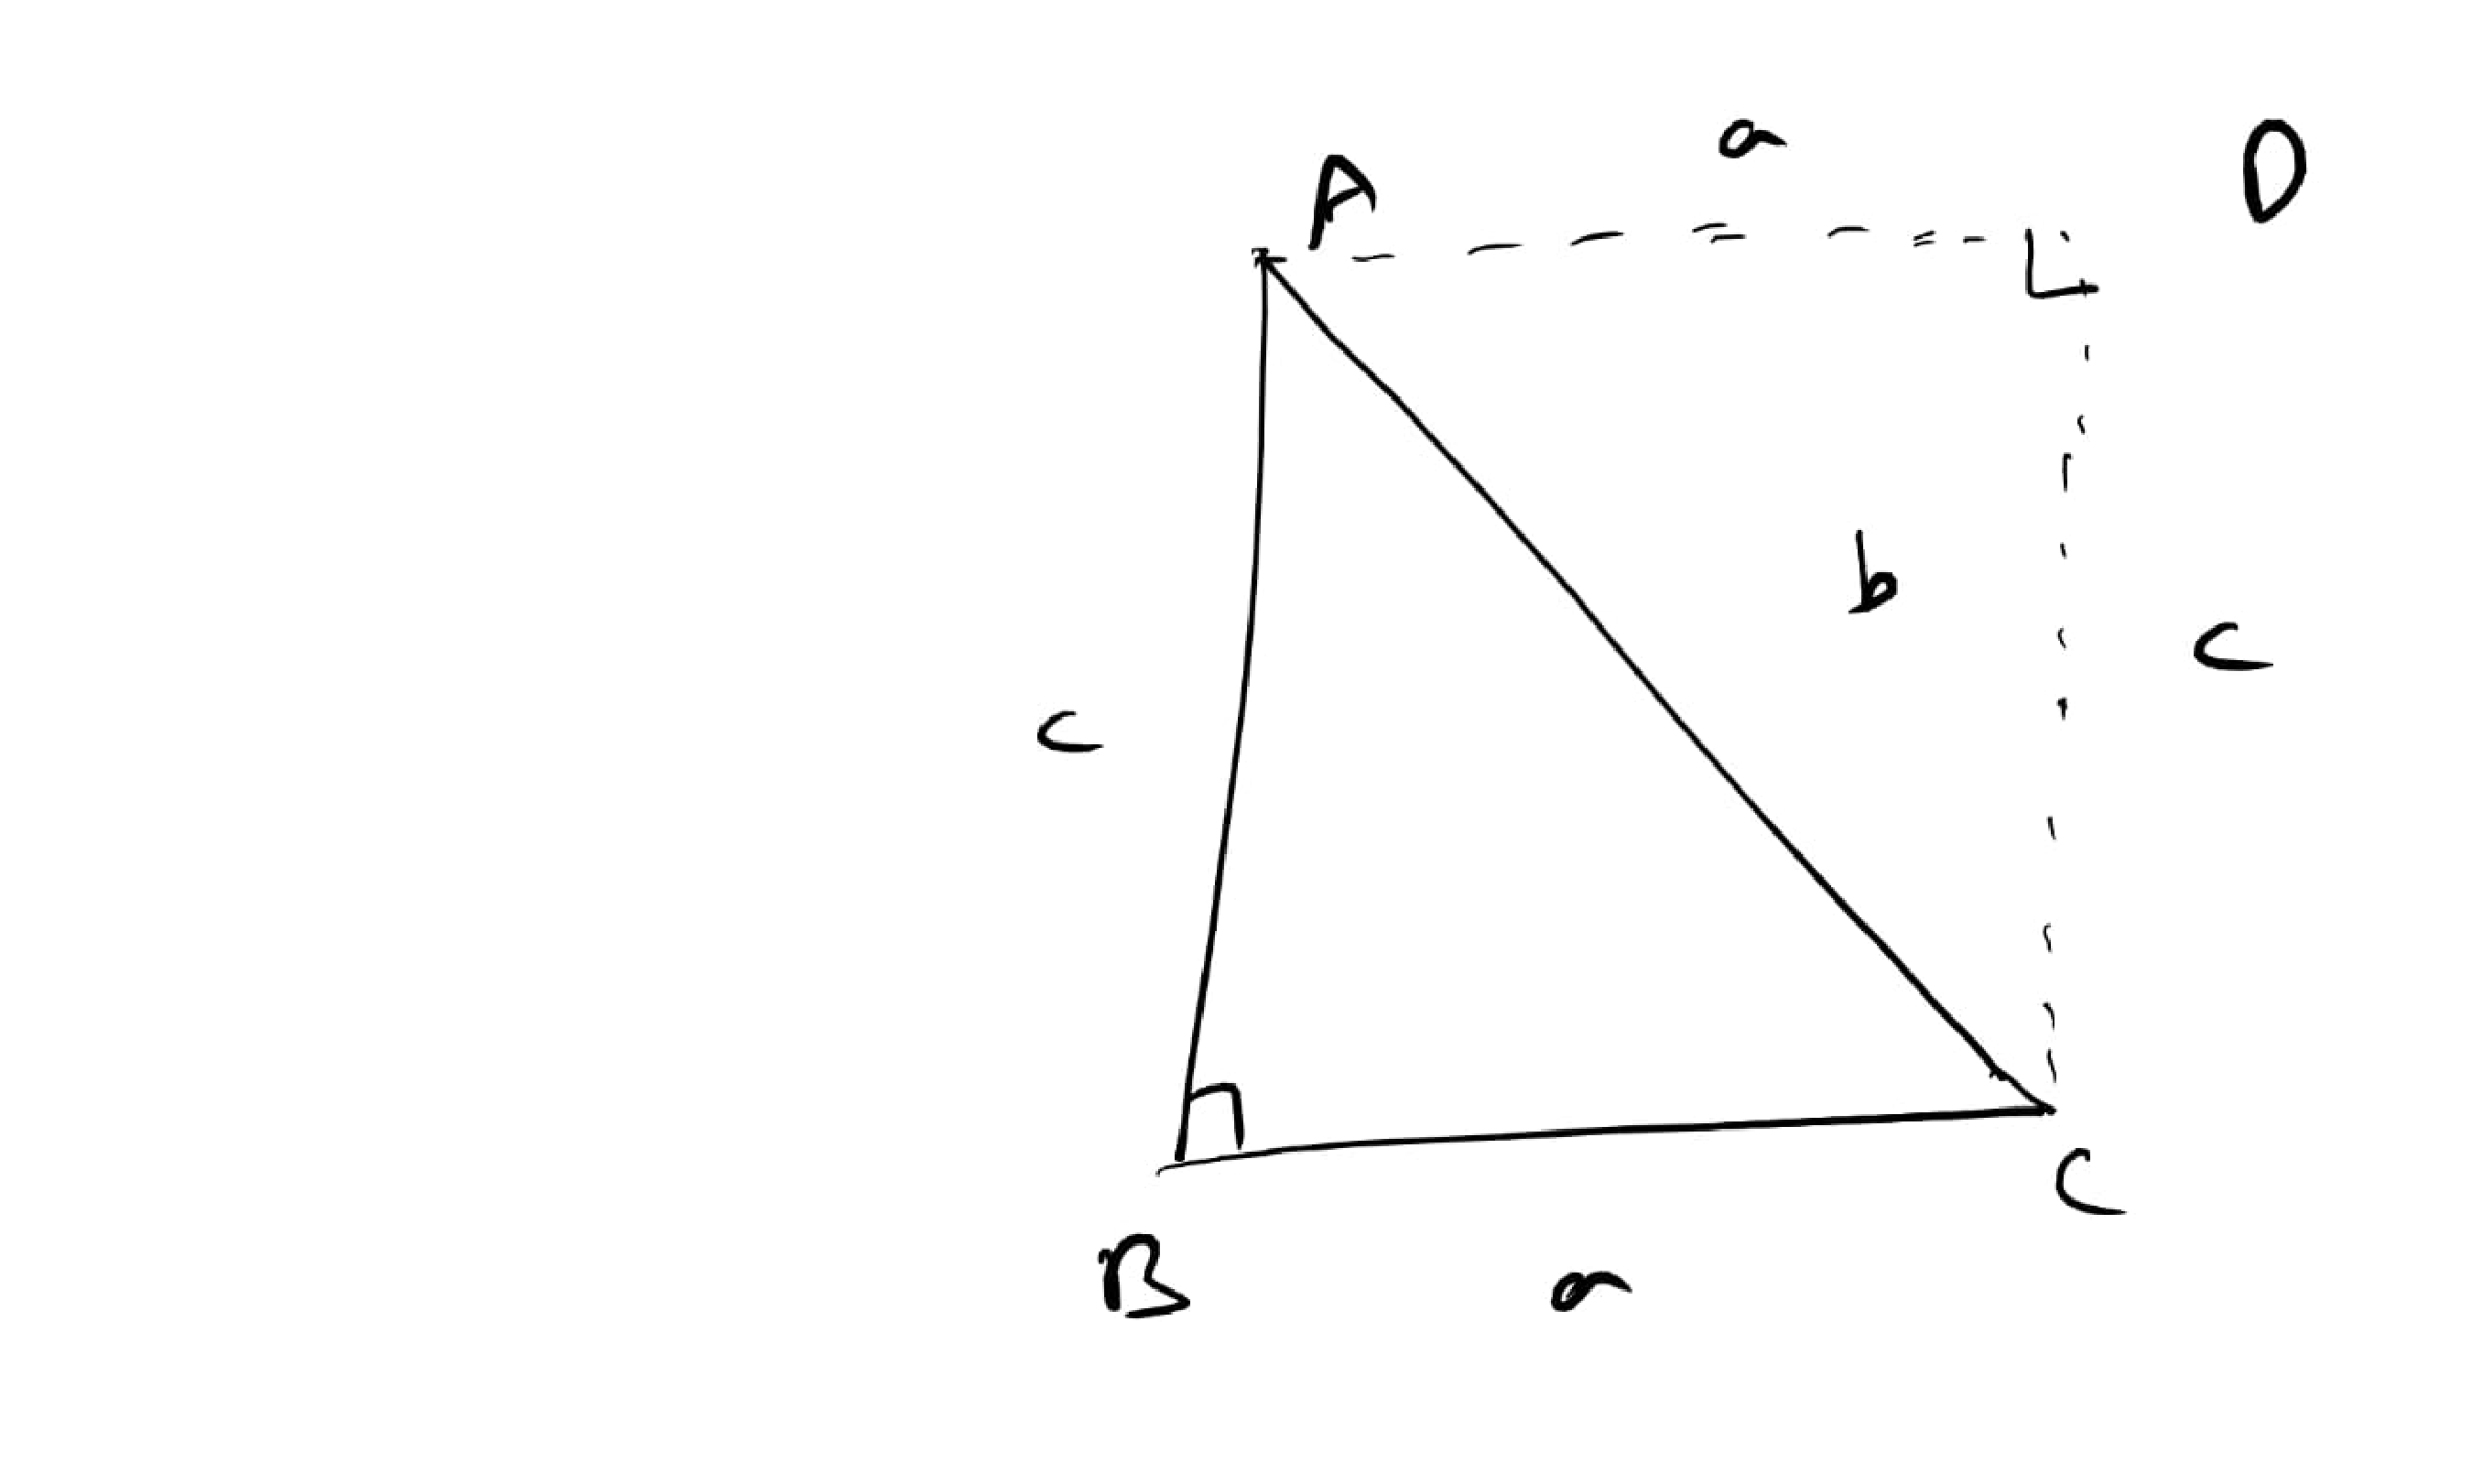
\includegraphics[width=\columnwidth]{./triangle/figs/tri_right_area.eps}
%\caption{}
%\label{fig:tri_right_area}
%\end{figure}
%%
%For any $\triangle ABC$, as shown in Fig.  \ref{fig:tri_area}, the area can be obtained as
%%
%\begin{align}
%\text{ar}\triangle ABC&=\frac{1}{2}xh+\frac{1}{2}yh 
%\\
%\frac{1}{2}\brak{x+y}h = \frac{1}{2}ah
%\end{align} 
%%

%
%\begin{figure}[!ht]
%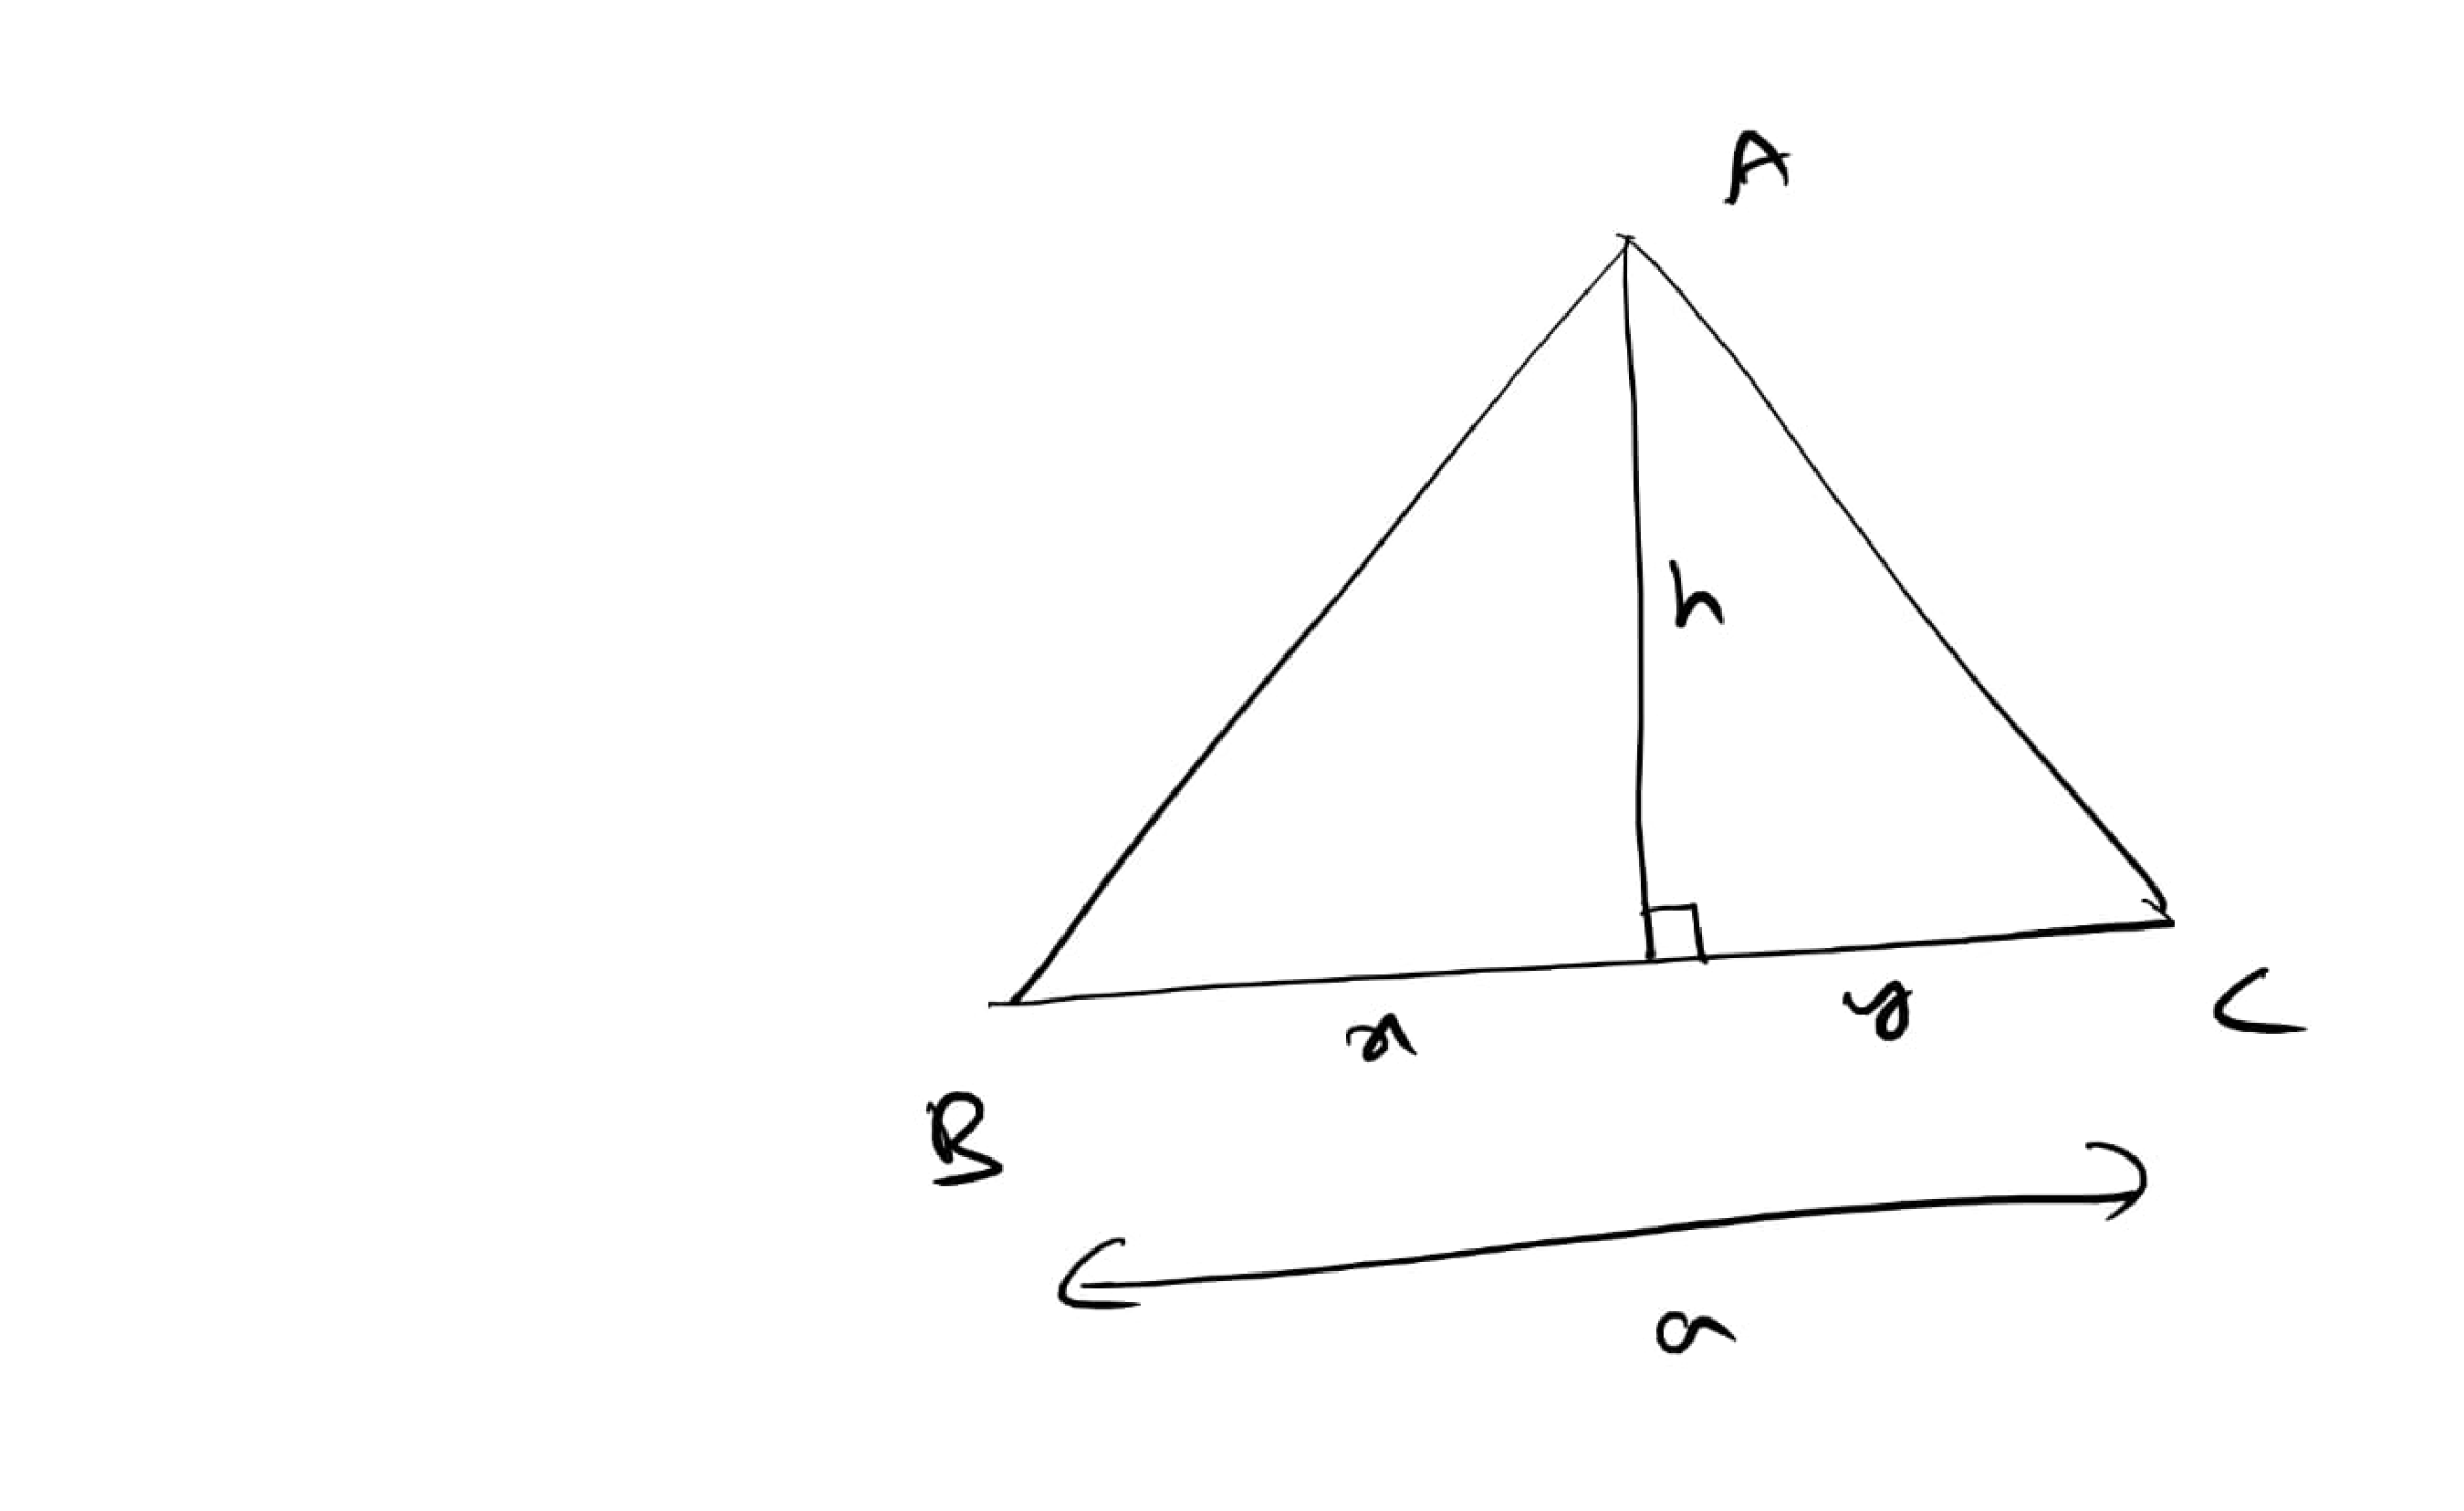
\includegraphics[width=\columnwidth]{./triangle/figs/tri_area.eps}
%\caption{}
%\label{fig:tri_area}
%\end{figure}
%
\item Find the area of a triangle whose vertices are 
$\vec{A}=\myvec{1\\-1}, 
\vec{B} = \myvec{-4\\6}$ and
$ 
\vec{C} = \myvec{-3\\-5}
$.
%
\\
\solution
  Using Hero's formula, the following code computes the area of the  triangle as 24.
%
\begin{lstlisting}
codes/triangle/area_tri.py
\end{lstlisting}
%
%\item A median of a triangle divides it into two triangles of equal areas.
%\\
%\solution In $\triangle ABC$, let $AD$
%
\item Find the area of a triangle formed by the vertices $\vec{A}=\myvec{5\\2}, \vec{B}=\myvec{4\\7}, \vec{C}=\myvec{7\\-4}$.
%\\
\solution  The area of $\triangle ABC$ is also obtained  in terms of the  {\em magnitude} of the determinant of the matrix $\vec{M}$ in  \eqref{eq:tri_geo_ex_diff_mat} as
%
\begin{align}
\frac{1}{2}\mydet{\vec{M}}
\end{align}
The computation is done in \textbf{area\_tri.py}
\item Find the area of a triangle formed by the points $\vec{P}=\myvec{-1.5\\3}, \vec{Q}=\myvec{6\\-2}, \vec{R}=\myvec{-3\\4}$.
\\
\solution Another formula for the area of $\triangle ABC$  is
%
\begin{align}
\frac{1}{2}\mydet{1 & 1 & 1\\ \vec{A} & \vec{B} & \vec{C} }
\end{align}
%
\item Find the area of a triangle having the points
%
\begin{align}
\vec{A} = \myvec{1\\1 \\1},
\vec{B} = \myvec{1\\2 \\3},
\vec{C} = \myvec{2\\ 3\\1}
\end{align}
%
as its vertices.
\\
\solution The area of a triangle using the {\em vector product} is obtained as
\begin{align}
\frac{1}{2}\norm{\brak{\vec{B}-\vec{A}}\times \brak{\vec{C}-\vec{A}}}
\end{align}
%
For any two vectors $\vec{a}=\myvec{a_1\\a_2\\a_3}, \vec{b}=\myvec{b_1\\b_2\\b_3}$, 
\begin{align}
\label{eq:tri_cross_prod}
\vec{a}\times \vec{b} = \myvec{0 & -a_3 & a_2 \\ a_3 & 0 & -a_1 \\ -a_2 & a_1 & 0}\myvec{b_1\\b_2\\b_3}
\end{align}
%
The following code computes the area using the vector product.
%
\begin{lstlisting}
codes/triangle/area_tri_vec.py
\end{lstlisting}
%
%
\item The centroid of a $\triangle ABC$ is at the point \myvec{1\\1\\1}.  If the coordinates of $\vec{A}$ and $\vec{B}$ are \myvec{3\\-5\\7} and \myvec{-1\\7\\-6}, respectively, find the coordinates of the point $\vec{C}$.
%
\\
\solution The centroid of $\triangle ABC$ is given by
\begin{align}
\label{eq:tri_geo_ex_centroid}
\vec{O} = \frac{\vec{A}+\vec{B}+\vec{C}}{3}
\end{align}
%
Thus, 
\begin{align}
\vec{C} = 3\vec{C}-\vec{A}-\vec{B}
\end{align}
%
\item Show that the points 
\begin{align}
\vec{A} = \myvec{2\\-1 \\1},
\vec{B} = \myvec{1\\-3 \\-5},
\vec{C} = \myvec{3\\ -4\\-4}
\end{align}
%
are the vertices of a right angled triangle.
\\
\solution 
The following code plots Fig. \ref{fig:triangle_3d}
%
\begin{lstlisting}
codes/triangle/triangle_3d.py
\end{lstlisting}
%
\begin{figure}[!ht]
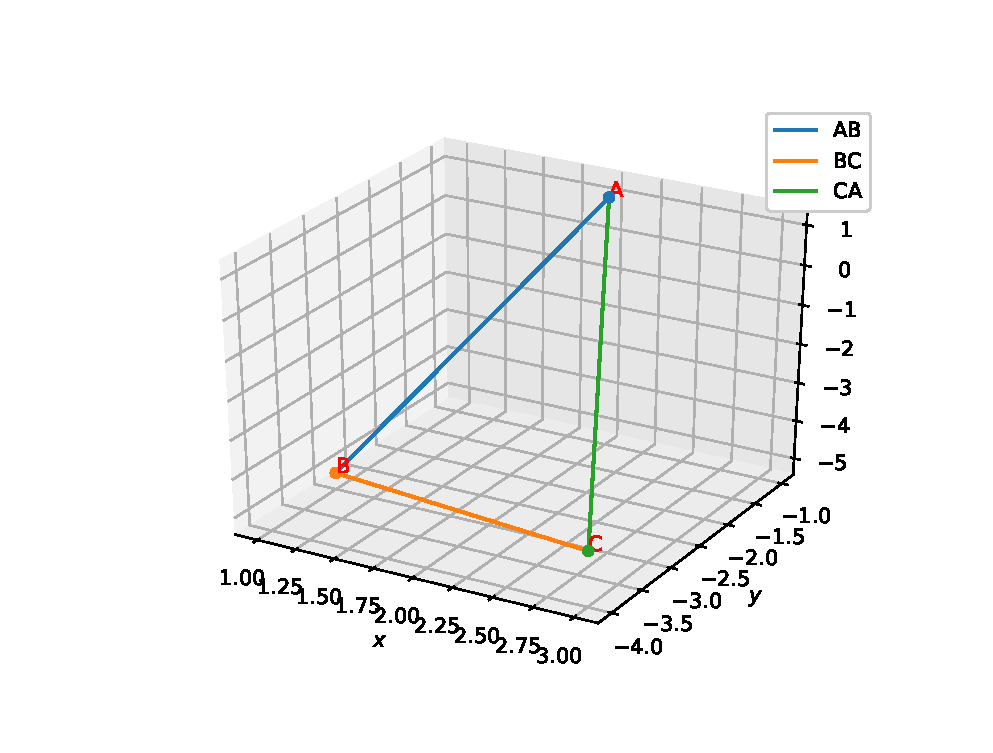
\includegraphics[width=\columnwidth]{./triangle/figs/triangle_3d.eps}
\caption{}
\label{fig:triangle_3d}
\end{figure}
%
From the figure, it appears that $\triangle ABC$ is right angled at $\vec{C}$.  Since 
\begin{align}
\brak{\vec{A}-\vec{C}}^T\brak{\vec{B}-\vec{C}}&=0
\end{align}
%
it is proved that the triangle is indeed right angled.
 \item Are the points 
\begin{align}
\vec{A} = \myvec{3\\6 \\9},
\vec{B} = \myvec{10\\20 \\30},
\vec{C} = \myvec{25\\ -41\\5},
\end{align}
%
the vertices of a right angled triangle?
%
%
\end{enumerate}
%
 
%\subsection{Triangle Exercises}
%\renewcommand{\theequation}{\theenumi}
\begin{enumerate}[label=\arabic*.,ref=\thesubsection.\theenumi]
\numberwithin{equation}{enumi}
%
\item Draw the graphs of the equations 
\begin{align}
\myvec{1 & -1}\vec{x} + 1 &= 0 
\\
\myvec{ 3 & 2} - 12 &= 0
\end{align}
%
 Determine the coordinates of the vertices of the triangle formed by these lines and the x-axis, and shade the triangular region.
%
\item In a $\triangle ABC, \angle C = 3 \angle B = 2 (\angle A + \angle B)$. Find the three angles. 
\item Draw the graphs of the equations $5x – y = 5$ and $3x – y = 3$. Determine the co-ordinates of the vertices of the triangle formed by these lines and the y axis.

\item The vertices of $\triangle PQR$ are 

$
\vec{P} = \myvec{2 \\1},
\vec{Q} = \myvec{-2\\3},
\vec{R} = \myvec{4\\5}.
$
Find the equation of the median through the vertex $\vec{R}$.
\item In the $\triangle ABC$ with vertices
$
\vec{A}=\myvec{2\\3}, 
\vec{B}=\myvec{4\\-1},
 \vec{C}=\myvec{1\\2}
$,
find the equation and length of the altitude from the vertex $\vec{A}$.
\item Find the area of the triangle whose vertices are
\begin{enumerate}
\item \myvec{2\\3}, \myvec{-1\\0},  \myvec{2\\-4}
\item  \myvec{-5\\-1},  \myvec{3\\-5},  \myvec{5\\2}
\end{enumerate}
\item Find the area of the triangle formed by joining the mid points o the sides of a triangle whose vertices are  \myvec{0\\-1},  \myvec{2\\1},  \myvec{0\\3}.
\item Verify that the median of $\triangle ABC$ with vertices $\vec{A}=\myvec{4\\-6},  \vec{B}=\myvec{3\\-2}$ and  $\vec{C} =  \myvec{5\\2}$ divides it into two triangles of equal areas.
\item The vertices of $\triangle ABC$ are $\vec{A}=\myvec{4\\6},  \vec{B}=\myvec{1\\5}$ and  $\vec{C} =  \myvec{7\\2}$.  A line is drawn to intersect sides $AB$ and $AC$ at $D$ and $E$ respectively, such that
\begin{align}
\frac{AD}{AB}=\frac{AE}{AC}= \frac{1}{4}
\end{align}
%
Find 
\begin{align}
\frac{\text{area of }\triangle ADE}{\text{area of }\triangle ABC}.
\end{align}
\item Let $\vec{A}=\myvec{4\\2},  \vec{B}=\myvec{6\\5}$ and  $\vec{C} =  \myvec{1\\4}$ be the vertices of $\triangle ABC$.
\begin{enumerate}
\item The median from $\vec{A}$ meets $BC$ at $\vec{D}$.  Find the coordinates of the point $\vec{D}$.
\item Find the coordinates of the point $\vec{P}$ on $AD$ such that $AP:PD = 2:1$.
\item Find the coordinates of the points $\vec{Q}$ and $\vec{R}$ on medians $BE$ and $CF$ respectively such that $BQ:QE = 2:1$ and $CR:RF = 2:1$.
\end{enumerate}
\item In $\triangle ABC$, Show that the centroid 
\begin{align}
\vec{O} = \frac{\vec{A}+\vec{B}+\vec{C}}{3}
\end{align}
\item Show that the points 
\begin{align}
\vec{A} = \myvec{2\\-1 \\1},
\vec{B} = \myvec{1\\-3 \\-5},
\vec{C} = \myvec{3\\ -4\\-4}
\end{align}
%
are the vertices of a right angled triangle.
\item In $\triangle ABC$, 
$
\vec{A} = \myvec{1\\2 \\3},
\vec{B} = \myvec{-1\\0 \\0},
\vec{C} = \myvec{0\\ 1\\2}.
$
Find $\angle B$.
\item Show that the vectors 
$
\myvec{2\\-1 \\1},
\myvec{1\\-3 \\-5},
\myvec{3\\ -4\\-4}
$
form the vertices of a right angled triangle.
\item Find the area of a triangle having the points 
$
\vec{A} = \myvec{1\\1 \\1},
\vec{B} = \myvec{1\\2 \\3}, \text{ and }
\vec{C} = \myvec{2\\ 3\\1}
$
as its vertices.
\item Find the area of a triangle with vertices
$
\vec{A} = \myvec{1\\1 \\2},
\vec{B} = \myvec{2\\3 \\5}, \text{ and }
\vec{C} = \myvec{1\\ 5\\5}
$
\item Find the direction vectors of the sides of a triangle with vertices
$
\vec{A} = \myvec{3\\5 \\-4},
\vec{B} = \myvec{-1\\1 \\2}, \text{ and }
\vec{C} = \myvec{-5\\ -5\\-2}
$
\item Without using the Pythagoras theorem, show that the points \myvec{4\\ 4}, \myvec{3\\ 5} and \myvec{–1\\ –1} are the vertices of a right angled triangle.
\item Check whether 
\begin{align}
\myvec{5\\-2}, \myvec{6\\4}, \myvec{7\\-2}
\end{align}
are the vertices of an isosceles triangle.
%

\end{enumerate}
%

 
%%
%\section{Quadrilateral}
%\subsection{Quadrilateral Examples}
%\renewcommand{\theequation}{\theenumi}
\begin{enumerate}[label=\arabic*.,ref=\thesubsection.\theenumi]
\numberwithin{equation}{enumi}
%

\item Show that the points $\vec{A} = \myvec{1\\7}, \vec{B} = \myvec{4\\2}, \vec{C}=\myvec{-1\\-1},\vec{D}= \myvec{-4\\4} $  are the vertices of a square.
\\
\solution By inspection, 
%
\begin{align}
\frac{\vec{A}+\vec{C}}{2}=\frac{\vec{B}+\vec{D}}{2} = \myvec{0\\3}
\end{align}
%
Hence, the diagonals $AC$ and $BD$ bisect each other.
%
Also, 
\begin{align}
\brak{\vec{A}-\vec{C}}^T
\brak{\vec{B}-\vec{D}} = 0
\end{align}
%
$\implies AC \perp BD $.  Hence $ABCD$ is a square.
\item If the points
$
\vec{A} = \myvec{6\\1}, 
\vec{B} = \myvec{8\\2}, 
\vec{C} = \myvec{9\\4}, 
\vec{D} = \myvec{p\\3}
$
are the vertices of a parallelogram, taken in order, find the value of $p$.
\\
\solution In the parallelogram $ABCD$, $AC$ and $BD$ bisect each other.  This can be used to find $p$.
\item If $\vec{A} = \myvec{-5\\7}, \vec{B} = \myvec{-4\\-5}, \vec{C} = \myvec{-1\\-6}, \vec{D} = \myvec{4\\5}$, find the area of the quadrilateral $ABCD$.
%
\\
\solution The area of  $ABCD$ is the sum of the areas of trianges ABD and CBD and is given by 
\begin{multline}
\frac{1}{2}\norm{\brak{\vec{A}-\vec{B}}\times \brak{\vec{A}-\vec{D}}}
\\
+
\frac{1}{2}\norm{\brak{\vec{C}-\vec{B}}\times \brak{\vec{C}-\vec{D}}}
\end{multline}
\item Show that the points 
$\vec{A} = \myvec{1\\2\\3},
 \vec{B} = \myvec{-1\\-2\\-1},
\vec{C} = \myvec{2\\3\\2},
\vec{D} = \myvec{4\\7\\6}.
$
are the vertices of a parallelogram $ABCD$ but it is not a rectangle.
%
\\
\solution Since the direction vectors
%
\begin{align}
\vec{A}-\vec{B}&= \vec{D}-\vec{C}
\\
\vec{A}-\vec{D}&= \vec{B}-\vec{C}
\end{align}
%
$AB \parallel CD$ and $AD \parallel BC$.  Hence $ABCD$ is a parallelogram.  However, 
%
\begin{align}
\brak{\vec{A}-\vec{B}}^T\brak{ \vec{A}-\vec{D}}\ne 0
\end{align}
%
Hence, it is not a rectangle.
The following code plots Fig. \ref{fig:quad_3d}
%
\begin{lstlisting}
codes/triangle/quad_3d.py
\end{lstlisting}
%
\begin{figure}[!ht]
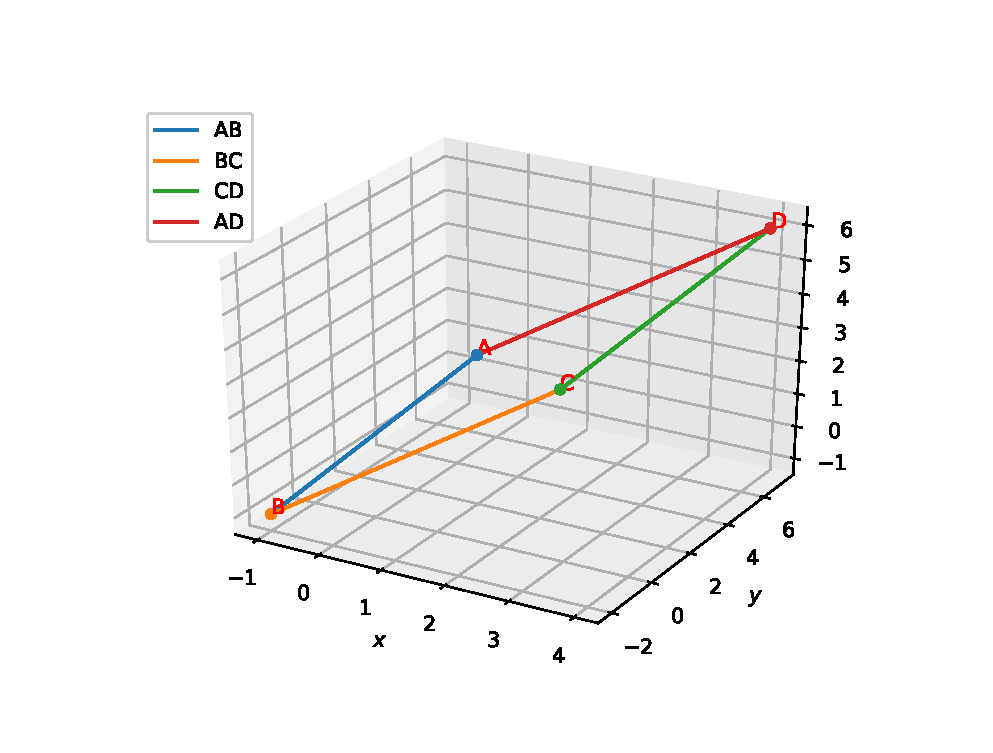
\includegraphics[width=\columnwidth]{./triangle/figs/quad_3d.eps}
\caption{}
\label{fig:quad_3d}
\end{figure}
%

\item Find the area of a parallelogram whose adjacent sides are given by the vectors \myvec{3\\1\\4} and \myvec{1\\-1\\1}.
%
\\
\solution  The area is given by 
%
\begin{align}
\frac{1}{2}\norm{\myvec{3\\1\\4} \times \myvec{1\\-1\\1}}
\end{align}
%
\end{enumerate}
%
 
%\subsection{Quadrilateral Geometry}
%%\renewcommand{\theequation}{\theenumi}
%\begin{enumerate}[label=\arabic*.,ref=\thesubsection.\theenumi]
%\numberwithin{equation}{enumi}

\item The two adjacent sides of a parallelogram are \myvec{2\\ -4 \\ -5} and  \myvec{1\\-2\\ -3}. Find the unit vector parallel to its diagonal.  Also, find its area.
%
\item Find the area of a parallelogram whose adjacent sides are determined by the vectors $\vec{a} = \myvec{1\\-1\\3}$ and $\vec{b}=\myvec{2\\-7\\1}$.
\item Verify if $\vec{A} = \myvec{3\\1}, \vec{B} = \myvec{6\\4}, \vec{C} = \myvec{8\\6}$ are points on a line.

%
%\end{enumerate}
%
 
%
\section{Constrained Optimization}
%\subsection{Equality Constraint}
\renewcommand{\theequation}{\theenumi}
\begin{enumerate}[label=\arabic*.,ref=\thesubsection.\theenumi]
\numberwithin{equation}{enumi}
%
\item Check whether –2 and 2 are zeroes of the polynomial $x + 2.$
\\
\solution Let 
%
\begin{align}
y &= x + 2
\implies \myvec{-1 & 1}\vec{x} &= 2
\end{align}
%
Thus, 
%
\begin{align}
y &= 0 
\\
\implies  x + 2 &=0
\\
\text{or, } x &= -2
\end{align}
%
Hence -2 is a zero. This is verified in Fig. \ref{fig:line_zeros}.
%
\begin{figure}[!ht]
\includegraphics[width=\columnwidth]{./line/figs/line_zeros.eps}
\caption{}
\label{fig:line_zeros}
\end{figure}
%
\item Find a zero of the polynomial $p(x) = 2x + 1$.
\\
\solution $p\brak{-\frac{1}{2}} = 0$.
%
%
\item Find four different solutions of the equation 
\label{prob:line_icept}
%
\begin{align}
\label{eq:line_iceptx}
\myvec{1 & 2}\vec{x} &= 6
\end{align}
%
\solution Let 
%
\begin{align}
\vec{x} = \myvec{a\\0}
\end{align}
%
Substituting in \eqref{eq:line_iceptx}, 
%
\begin{align}
\myvec{1 & 2} \myvec{a\\0}&= 6
\\
\implies a &=6
\end{align}
%
Simiarly, substituting 
%
\begin{align}
\vec{x} &= \myvec{0\\b},
\end{align}
%
in \eqref{eq:line_iceptx}, 
%
%
\begin{align}
b =3
\end{align}
%
More solutions can be obtained in a similar fashion.
%
\item Draw the graph of 
%
\begin{align}
\myvec{1 & 1}\vec{x} &= 7
\end{align}
%
\solution The intercepts on the x and y-axis can be obtained from Problem \ref{prob:line_icept}
as
%
\begin{align}
\vec{A} = \myvec{7\\0}
\vec{B} = \myvec{0\\7}
\end{align}
%
The following python code can be used to draw the graph in Fig. \ref{fig:line_icept}.
%
\begin{lstlisting}
codes/line/line_icept.py
\end{lstlisting}
%
\begin{figure}[!ht]
\includegraphics[width=\columnwidth]{./line/figs/line_icept.eps}
\caption{}
\label{fig:line_icept}
\end{figure}
%
%
\item Two rails are represented by the equations 
\label{prob:line_mat_eq}
\begin{align}
\label{eq:line_mat_eq}
\begin{split}
\myvec{1 & 2}\vec{x}  &= 4 \text{ and}
\\
\myvec{ 2 & 4}\vec{x} &=  12 . 
\end{split}
\end{align}
%
Will the rails cross each other?
%
\\
\solution The above equations can be expressed as the matrix equation
\begin{align}
\myvec{1 & 2\\2 & 4} \vec{x} = \myvec{4\\12}
\end{align}
%
The augmented matrix for the above equation is row reduced as follows
\begin{align}
\myvec{1 & 2 & 4\\2 & 4 & 12} 
\xleftrightarrow {R_2\leftarrow \frac{R_2}{2}}\myvec{1 & 2 & 4\\1 & 2 & 6} 
\\
%\myvec{1 & 2 & 4\\2 & 4 & 12} 
\xleftrightarrow {R_2\leftarrow R_2 - R_1}\myvec{1 & 2 & 4\\0 & 0 & 2} 
\label{eq:line_aug}
\end{align}
%
$\because$ row reduction of the $2\times 3$ matrix
%
\begin{align}
\myvec{1 & 2 & 4\\2 & 4 & 12} 
\end{align}
%
results in a matrix with 2 nonzero rows, its rank is 2.  Similarly, the rank of the matrix 
%
\begin{align}
\myvec{1 & 2\\2 & 4} 
\end{align}
is 1, from \ref{eq:line_aug}. 
%
\begin{align}
\because rank \myvec{1 & 2\\2 & 4} \ne rank\myvec{1 & 2 & 4\\2 & 4 & 12},  
\end{align}
%
\eqref{eq:line_mat_eq} has no solution.
%
The equivalent python code is
%
\begin{lstlisting}
codes/line/line_check_sol.py
\end{lstlisting}
%
which plots Fig. \ref{fig:line_check_sol}, which shows that the rails are parallel.
%
\begin{figure}[!ht]
\includegraphics[width=\columnwidth]{./line/figs/line_check_sol.eps}
\caption{}
\label{fig:line_check_sol}
\end{figure}
%

\item Check whether the pair of equations 
\begin{align}
\label{eq:line_mat_eq_2}
\begin{split}
\myvec{1 & 3}\vec{x}  &= 6 \text{ and}
\\
\myvec{ 2 & -3}\vec{x} &= 12 
\end{split}
\end{align}
%
is consistent. 
\\
\solution The above equations can be expressed as the matrix equation
\begin{align}
\myvec{1 & 3\\2 & -3} \vec{x} = \myvec{6\\12}
\end{align}
%
The augmented matrix for the above equation is row reduced as follows
\begin{align}
\myvec{1 & 3 & 6\\2 & -3 & 12} 
\xleftrightarrow {R_2\leftarrow \frac{R_2-2R_1}{-9}}
%\myvec{1 & 3 & 6\\0 & -9 & 0} 
\\
\myvec{1 & 3 & 6\\0 & 1 & 0} 
\xleftrightarrow {R_1\leftarrow R_1 - 3R_2}\myvec{1 & 0 & 6\\0 & 1 & 0} 
\\
\implies \vec{x} = \myvec{6\\0}
\end{align}
%
which is the solution of \ref{eq:line_mat_eq}.
The python code in Problem \ref{prob:line_mat_eq}
%
%
can be used to plot Fig. \ref{fig:line_check_sol2}, which shows that the lines intersect.
%
\begin{figure}[!ht]
\includegraphics[width=\columnwidth]{./line/figs/line_check_sol2.eps}
\caption{}
\label{fig:line_check_sol2}
\end{figure}
%
%
\item Find whether the following pair of equations has no solution, unique solution or infinitely many solutions: 
%
\begin{align}
\label{eq:line_check_sol3}
\begin{split}
\myvec{5 & -8}\vec{x}  &= -1 \text{ and}
\\
\myvec{ 3 & -\frac{24}{5}}\vec{x} &= -\frac{3}{5}
\end{split}
\end{align}
%
\\
\solution The above equations can be expressed as the matrix equation
\begin{align}
\myvec{5 & -8\\3 & -\frac{24}{5}} \vec{x} = -\myvec{1\\ \frac{3}{5}}
\end{align}
%
The augmented matrix for the above equation is row reduced as follows
\begin{align}
\myvec{5 & -8 & -1 \\3 & -\frac{24}{5} & -\frac{3}{5}} 
\xleftrightarrow {R_2\leftarrow 5R_2}\myvec{5 & -8 & 1\\15 & -24 & -3} 
\\
%\myvec{5 & -8 & 1\\15 & -24 & -3} 
\xleftrightarrow {R_2\leftarrow R_2 - 3R_1}\myvec{5 & -8 & 1\\0 & 0 & 0} 
\end{align}
%
%
\begin{align}
\because rank \myvec{5 & -8\\3 & -\frac{24}{5}} &= rank \myvec{5 & -8 & 1 \\3 & -\frac{24}{5} & -\frac{3}{5}} 
\\
= 1 < dim \myvec{5 & -8\\3 & -\frac{24}{5}} =2,
\end{align}
%
\eqref{eq:line_check_sol3} has infinitely many solutions.
%
The python code in Problem \ref{prob:line_mat_eq}
%
%
can be used to plot Fig. \ref{fig:line_check_sol3}, which shows that the lines are the same.
%
\begin{figure}[!ht]
\includegraphics[width=\columnwidth]{./line/figs/line_check_sol3.eps}
\caption{}
\label{fig:line_check_sol3}
\end{figure}
%
%
\item Solve the following pair of equations
%
\begin{align}
\label{eq:line_check_sol_unique}
\myvec{7 & -15}\vec{x}  &= 2 
\\
\myvec{ 1 & 2}\vec{x} &= 3
\end{align}
%
\\
\solution The above equations can be expressed as the matrix equation
\begin{align}
\myvec{7 & -15\\1 & 2} \vec{x} = \myvec{2\\ 3}
\end{align}
%
The augmented matrix for the above equation is row reduced as follows
\begin{align}
\myvec{7 & -15 & 2\\1 & 2 & 3}
\xleftrightarrow {R_2\leftarrow 7R_2-R_1}\myvec{7 & -15 & 2\\0 & 29 & 19}
\\
\xleftrightarrow {R_1\leftarrow \frac{15R_2 29+ 29R_1}{29}}\myvec{7 & 0 & 2\\0 & 29 & 19} 
\\
\implies \vec{x} = \myvec{\frac{2}{7}\\\frac{19}{29}}
\end{align}
%
%

The python code in Problem \ref{prob:line_mat_eq}
%
%
can be used to plot Fig. \ref{fig:line_check_sol_unique}, which shows that the lines are the same.
%
\begin{figure}[!ht]
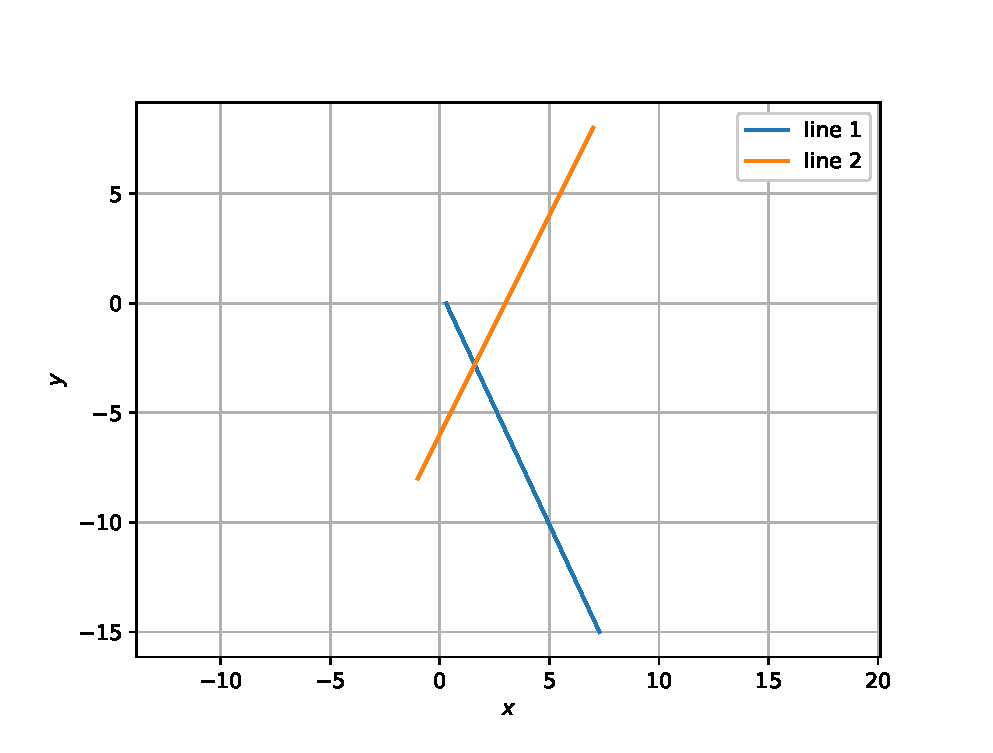
\includegraphics[width=\columnwidth]{./line/figs/line_check_unique.eps}
\caption{}
\label{fig:line_check_sol_unique}
\end{figure}
%
\item Find all possibe solutions of
\begin{align}
\label{eq:line_check_sol_nosol}
\begin{split}
\myvec{2 & 3 }\vec{x}&=8
\\
\myvec{4 & 6 }\vec{x}&=7
\end{split}
\end{align}
%
\\
\solution The above equations can be expressed as the matrix equation
\begin{align}
\myvec{2 & -3\\4 & 6} \vec{x} = \myvec{8\\ 7}
\end{align}
%
The augmented matrix for the above equation is row reduced as follows
\begin{align}
\myvec{2 & 3 & 8\\4 &  6 & 7} 
\xleftrightarrow {R_2\leftarrow R_2-2R_1}\myvec{2 & -3 & 8\\0 &  0 & -9} 
\\
\implies rank \myvec{2 & -3\\4 & 6} \ne \myvec{2 & 3 & 8\\4 &  6 & 7}. 
\end{align}
%
Hence, \eqref{eq:line_check_sol_nosol} has no solution.
The python code in Problem \ref{prob:line_mat_eq}
%
%
can be used to plot Fig. \ref{fig:line_check_nosol}, which shows that the lines are parallel.
%
\begin{figure}[!ht]
\includegraphics[width=\columnwidth]{./line/figs/line_check_nosol.eps}
\caption{}
\label{fig:line_check_nosol}
\end{figure}

\item For which values of p does the pair of equations given below has unique solution?
\begin{align}
\label{eq:line_det_unique}
\begin{split}
\myvec{4 & p }\vec{x}&=-8
\\
\myvec{2 & 2 }\vec{x}&=-2
\end{split}
\end{align}
%
\solution \eqref{eq:line_det_unique} has a unique solution 
\begin{align}
\iff \mydet{4 & p \\ 2 & 2} \ne 0
\\
\text{or, } p \ne 4
\end{align}
%
\item For what values of $k$ will the following pair of linear equations have infinitely many solutions?
%
\begin{align}
\label{eq:line_det_inf}
\begin{split}
\myvec{k & 3 }\vec{x}&=k-3
\\
\myvec{12 & k }\vec{x}&=k
\end{split}
\end{align}
%
\solution The first condition for \eqref{eq:line_det_inf} to have infinite solutions is 
%
\begin{align}
\label{eq:line_det_inf_cond}
\mydet{k & 3 \\12 & k  } &= 0
\\
\implies k^2 = 36, \text{or, } k = \pm 6
\end{align}
%
For $k = 6$, 
%
the augmented matrix for the above equation is row reduced as follows
\begin{align}
\myvec{6 & 3 & 3\\12 &  6 & 6} 
\xleftrightarrow {R_2\leftarrow R_2-2R_1}\myvec{6 & 3 & 3\\0 &  0 & 0} 
\end{align}
%
indicating that \eqref{eq:line_det_inf} has infinite number of solutions. For $k = -6$, the augmented matrix is 
\begin{align}
\myvec{6 & 3 & -9\\12 &  6 & -6} 
\xleftrightarrow {R_2\leftarrow R_2-2R_1}\myvec{6 & 3 & -9\\0 &  0 & 12} 
\end{align}
indicating that \eqref{eq:line_det_inf} has no solution
%
Thus, \eqref{eq:line_det_inf_cond} is a necessary condition but not sufficient.
%
\item Find the values of $x, y, z$ such that 
\begin{align}
\myvec{x\\2\\z}= \myvec{2\\y\\1}
\end{align}
%
\solution $x = 2, y=2, z=1$.
%
\item If
\begin{align}
\vec{a} = \myvec{1\\2}, \vec{b} = \myvec{2\\1},
\end{align}
verify if  
\begin{enumerate}
\item $\norm{\vec{a}}=\norm{\vec{b}}$

\item $\vec{a}=\vec{b}$
\end{enumerate}
%
\solution
\begin{enumerate}
\item $\norm{\vec{a}}=\norm{\vec{b}},\vec{a}\ne\vec{b}$.
\end{enumerate}
\item Find a unit vector in the  direction of \myvec{2\\3\\1}.
%
\\
\solution The unit vector is given by 
\begin{align}
\frac{\myvec{2\\3\\1}}{\norm{\myvec{2\\3\\1}}} = \frac{1}{\sqrt{14}}\myvec{2\\3\\1}
\end{align}
%
%
\item Find a unit vector in the direction of \myvec{2\\-1\\-2}.
%
\item Find a unit vector in the direction of the line passing through \myvec{-2\\4\\-5} and $\myvec{1\\2\\3}$.
%
\item Find a vector $\vec{x}$ in the direction of \myvec{1\\-2} such that $\norm{\vec{x}} = 7$.
%
\solution Let $\vec{x} = k\myvec{1\\-2}$.  Then 
%
\begin{align}
\norm{\vec{x}} &= \abs{k}\norm{\myvec{1\\-2}}= 7
\\
\implies \abs{k} &= \frac{7}{\sqrt{5}}
\\
\text{or, } \vec{x} &= \frac{7}{\sqrt{5}}\myvec{1\\-2}
\end{align}
%

\item Find a unit vector in the direction of $\vec{a}+\vec{b}$, where 
%
\begin{align}
\vec{a} = \myvec{2\\2\\-5}, \vec{b} = \myvec{2\\1\\3}.
\end{align}
%
\item Find a unit vector in the direction of 
%
\begin{align}
\myvec{1\\1\\-2}.
\end{align}
%
\item Find the direction vector of $PQ$, where 
\begin{align}
\vec{P} = \myvec{2\\3\\0},
\vec{Q} = \myvec{-1\\-2\\-4}
\end{align}
%
\solution The direction vector of $PQ$ is 
%
\begin{align}
\vec{P}-\vec{Q} = \myvec{3\\5\\4},
\end{align}
%

\item Verify if $\vec{A} = \myvec{3\\1}, \vec{B} = \myvec{6\\4}, \vec{C} = \myvec{8\\6}$ are points on a line.
\\
\solution Refer to Problem \ref{prob:tri_exam_coll_pts}.

\item Find the condition for $\vec{x} = \myvec{x_1\\x_2}$ to be equidistant from the points $\myvec{7\\1}, \myvec{3\\5}$.
\label{prob:line_perp_bisect}
%
\\
\solution From the given information,
%
\begin{align}
\norm{\vec{x}-\myvec{7\\1}}^2&=\norm{\vec{x}-\myvec{3\\5}}^2
\end{align}
\begin{multline}
\implies \norm{\vec{x}}^2 + \norm{\myvec{7\\1}}^2-2\myvec{7&1}\vec{x} 
\\= 
 \norm{\vec{x}}^2 + \norm{\myvec{3\\5}}^2-2\myvec{3&5}\vec{x} 
\end{multline}
%
which can be simplified to obtain
\begin{align}
\label{eq:line_p_bisect}
\myvec{1 & -1}\vec{x} = 2
\end{align}
%
which is the desired condition.  
The following code plots Fig. \ref{fig:line_perp_bisect}clearly showing that the above equation 
%\eqref{eq:line_p_bisect}
 is the perpendicular bisector of $AB$.

%
\begin{lstlisting}
codes/line/line_perp_bisect.py
\end{lstlisting}
%
\begin{figure}[!ht]
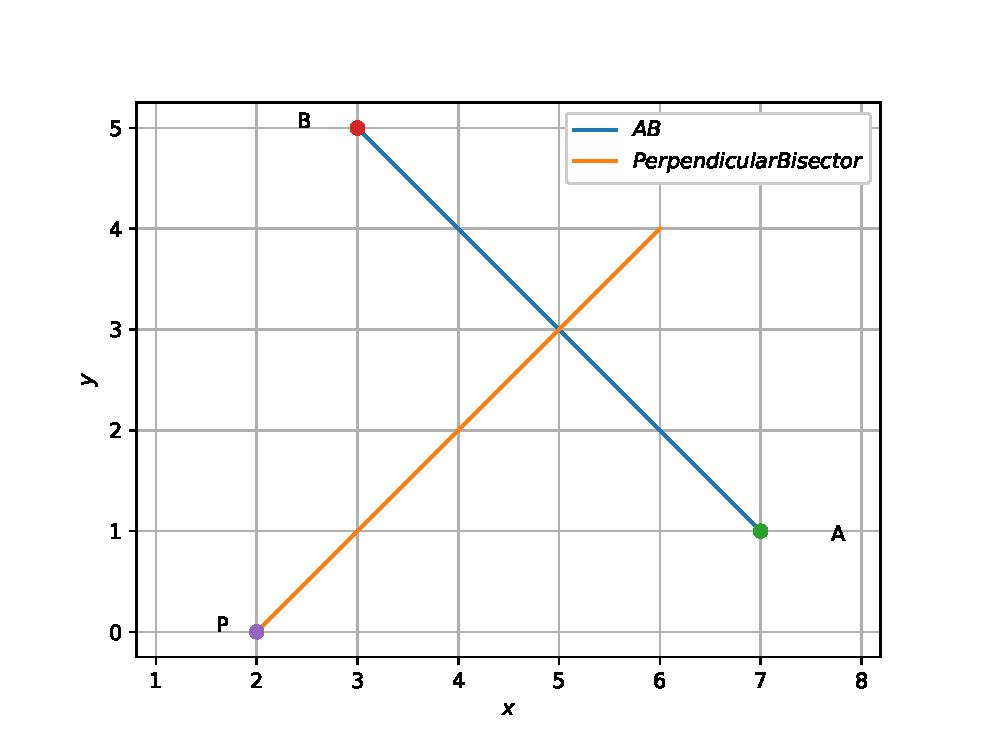
\includegraphics[width=\columnwidth]{./line/figs/line_perp_bisect.eps}
\caption{}
\label{fig:line_perp_bisect}
\end{figure}
%

\item Find a point on the $y$-axis which is equidistant from the points $\vec{A} = \myvec{6\\5}, \vec{B} = \myvec{-4\\3}$.
\\
\solution Choose $\vec{x} = \myvec{0\\y}$ and follow the approach in Problem \eqref{prob:line_perp_bisect}. Solve for $y$.

\item Draw a line segement of length 7.6 cm and divide it in the ratio $5:8$.
\\
\solution Let the end points of the line be 
\begin{align}
\vec{A} = \myvec{0\\0}, \vec{B} = \myvec{7.6\\0}
\end{align}
From \eqref{eq:tri_geo_ex_caorth_section},
the point $\vec{C}$
\begin{align}
\label{eq:line_section_form}
\vec{C} = \frac{k \vec{B} + \vec{A}}{k+1}
\end{align}
If $\vec{C}$ divides $AB$ in the ratio 
\begin{align}
 m = \frac{5}{8},
\end{align}
then,
\begin{align}
\label{eq:line_section_form_m}
\frac{\norm{\vec{C}-\vec{A}}^2}{\norm{\vec{B}-\vec{C}}^2} &= m^2
\\
\implies \frac{\frac{k^2\norm{\vec{B}-\vec{A}}^2}{\brak{k+1}^2}}{\frac{\norm{\vec{B}-\vec{A}}^2}{\brak{k+1}^2}} &=m^2
\\
\implies k = m &
\end{align}
upon substituting from \eqref{eq:line_section_form_m} and simplifying. \eqref{eq:line_section_form} is known as the section formula.
%
The following code plots Fig. \ref{fig:section}
\begin{lstlisting}
codes/line/draw_section.py
\end{lstlisting}
\begin{figure}[!ht]
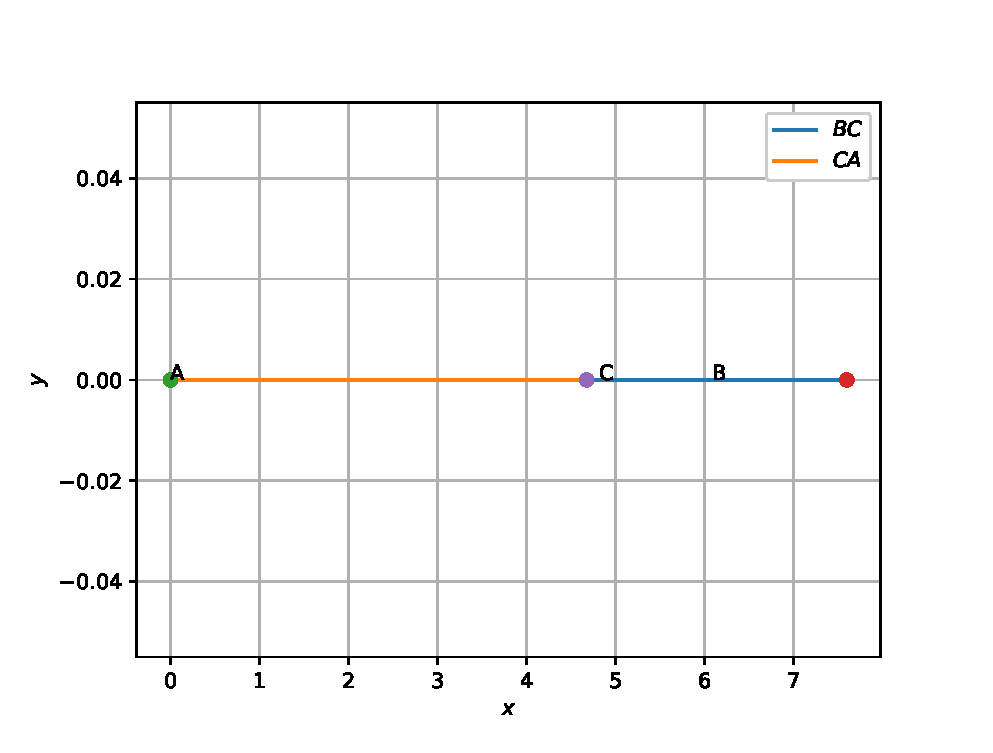
\includegraphics[width=\columnwidth]{./line/figs/section.eps}
\caption{}
\label{fig:section}
\end{figure}
\item Find the coordinates of the point which divides the line segment joining the points \myvec{4\\-3} and \myvec{8\\5} in the ratio $3:1$ internally.
\\
\solution Using \eqref{eq:line_section_form},
the desired point is 
\begin{align}
\vec{P} = \frac{3 \myvec{4\\-3} + \myvec{8\\5}}{4}
\end{align}
\item In what ratio does the point \myvec{-4\\6} divide the line segment joining the points 
%
\begin{align}
\vec{A} = \myvec{-6\\10},
\vec{B} = \myvec{3\\-8}
\end{align}
%
\\
\solution Use \eqref{eq:line_section_form}.
\item Find the coordinates of the points of trisection of the line segement joining the points
%
\begin{align}
\vec{A} = \myvec{2\\-2},
\vec{B} = \myvec{-7\\4}
\end{align}
%
\\
\solution Using \eqref{eq:line_section_form}, the coordinates are
%
\begin{align}
\label{eq:line_section_form_tri}
\vec{P} &= \frac{2 \vec{A} + \vec{B}}{3}
\\
\vec{Q} &= \frac{ \vec{A} + 2\vec{B}}{3}
\end{align}
%

\item Find the ratio in which the y-axis divides the line segment joining the points \myvec{5\\-6} and \myvec{-1\\-4}.
\\
\solution Let the corresponding point on the $y$-axis be$\myvec{0\\y}$. If the ratio be $k:1$,
using \eqref{eq:line_section_form}, the coordinates are
%
\begin{align}
\myvec{0\\y} &= k\myvec{5\\-6}+ \myvec{-1\\-4}
\\
\implies 0 &= 5k-1 \implies k = \frac{1}{5}
\end{align}
%


\item Find the value of $k$ if the points $\vec{A}=\myvec{2\\3}, \vec{B}=\myvec{4\\k}$ and $\vec{C}=\myvec{6\\-3}$ are collinear.
\\
\solution Forming the matrix in \eqref{eq:tri_geo_ex_diff_mat},
\begin{align}
\vec{M} = \myvec{\vec{B}-\vec{A} & \vec{B}-\vec{A}}^T 
= \myvec{2 & k-3\\4 & -6}&
\\
\xleftrightarrow {R_2\leftarrow \frac{R_2}{2}}\myvec{2 & k-3\\2 & -3}
\xleftrightarrow {R_2\leftarrow R_2-R_1}\myvec{2 & k-3\\0 & -k}&
\\
\implies rank(\vec{M})= 1 \iff R_2 = \vec{0}, \text{or }k = 0 &
\end{align}

\item Find the direction vectors and slopes of the lines passing through the points
%
\begin{enumerate}
\item \myvec{3\\-2} and \myvec{-1\\4}.
\item \myvec{3\\-2} and \myvec{7\\-2}.
\item \myvec{3\\-2} and \myvec{3\\4}.
\item Making an inclination of $60\degree$ with the positive direction of the x-axis.
\end{enumerate}
%
\solution
\begin{enumerate}
\item If the direction vector is 
\begin{align}
\myvec{1\\m}, 
\end{align}
%
the slope is $m$. Thus, the direction vector is
\begin{align}
\myvec{-1\\4} - \myvec{3\\-2} &= \myvec{-4\\6} = -\frac{1}{4} \myvec{-4\\6} 
\\
&=  \myvec{1\\-\frac{3}{2}} \implies m = -\frac{3}{2}
\end{align}
%
\item The direction vector is
\begin{align}
\myvec{7\\-2} - \myvec{3\\-2} &= \myvec{4\\0} 
\\
&=  \myvec{1\\0} \implies m = 0
\end{align}
%
\item The direction vector is
\begin{align}
\myvec{3\\4} - \myvec{3\\-2} &= \myvec{0\\6} 
\\
&=  \myvec{1\\ \infty} \implies m = \infty
\end{align}
%
\item The slope is $m = \tan 60 \degree = \sqrt{3}$ and the  direction vector is
\begin{align}
\myvec{1\\\sqrt{3}}
\end{align}
\end{enumerate}
\item If the angle between two lines is $\frac{\pi}{4}$ and the slope of one of the lines is $\frac{1}{4}$ find the slope of the other line.
\\
\solution The angle $\theta$ between two lines is given by 
%
\begin{align}
\tan \theta &= \frac{m_1-m_2}{1+m_1m_2}
\\
\implies 1 &= \frac{m_1-\frac{1}{4}}{1+\frac{m_1}{4}}
\\
\text{or } m_1 &= \frac{5}{3} 
\end{align}
%
\item The line through the points \myvec{-2\\6} and \myvec{4\\8} is perpendicular to the line through the points \myvec{8\\12} and $\myvec{x\\24}$.  Find the value of $x$.
%
\\
\solution Using \eqref{eq:tri_geo_ex_orth}
\begin{align}
\cbrak{\myvec{-2\\ 6}-\myvec{4\\8}}^T \cbrak{\myvec{8\\ 12}-\myvec{x\\24}}=  0 
\end{align}
%
which can be used to obtain $x$.
\item Two positions of time and distance are recorded as, when $T = 0, D = 2$ and when $T = 3, D = 8$. Using the concept of slope, find law of motion, i.e., how distance depends upon time.
%
\\
\solution The equation of the line joining the points $\vec{A}=\myvec{0\\2}$ and $\vec{B}=\myvec{3\\8}$ is obtained as
%
\begin{align}
\label{eq:line_two_pt}
\vec{x} &= \vec{A}+\lambda\brak{\vec{B}-\vec{A}}
\\
\implies \myvec{T\\D} &= \myvec{0\\2}-\lambda\myvec{-3\\-6}
\end{align}
%
which can be expressed as
\begin{align}
\myvec{2 & -1}\myvec{T\\D} &= \myvec{2 & -1}\myvec{0\\2}\\
\implies \myvec{2 & -1}\myvec{T\\D} &= -2
\\
\implies D = 2+2T
\end{align}
%
\item Find the equations of the lines parallel to the axes and passing through $\vec{A}=\myvec{-2\\3}$.
%
\\
\solution The line parallel to the x-axis has direction vector $\vec{m}=\myvec{1\\0}$.  Hence,its equation is obtined as
\begin{align}
%
\label{eq:line_dir_vec}
\vec{x} = \myvec{-2\\3} + \lambda_1\myvec{1\\0}
\end{align}
%
Similarly, the equation of the line parallel to the y-axis can be obtained as
\begin{align}
\vec{x} = \myvec{-2\\3} + \lambda_1\myvec{0\\1}
\end{align}
%
The following code plots Fig. \ref{fig:line_parallel_axes}
%
\begin{lstlisting}
codes/line/line_parallel_axes.py
\end{lstlisting}
%
\begin{figure}[!ht]
\includegraphics[width=\columnwidth]{./line/figs/line_parallel_axes.eps}
\caption{}
\label{fig:line_parallel_axes}
\end{figure}

\item Find the equation of the line through $\vec{A}=\myvec{– 2\\ 3}$ with slope –4.
\\
\solution The direction vector is $\vec{m} = \myvec{1\\-4}$.  Hence, the normal vector
\begin{align}
\label{eq:line_norm_dir}
\vec{n} &= \myvec{0&-1\\1&0}\vec{m} 
\\
&= \myvec{4\\1}
\end{align}
%
The equation of the line in terms of the normal vector is then obtained as
\begin{align}
\label{eq:line_norm_vec}
\vec{n}^T\brak{\vec{x}-\vec{A}} &= 0
\\
\implies \myvec{4 & 1} \vec{x} &= -5
\end{align}
%
\item Write the equation of the line through the points \myvec{1\\-1} and \myvec{3\\5}.
%
\\
\solution Use \eqref{eq:line_dir_vec}.
\item Write the equation of the lines for which $\tan \theta = \frac{1}{2}$, where $\theta$ is the inclination of the line and 
\label{prob:line_intercept}
\begin{enumerate}
\item y-intercept is $-\frac{3}{2}$
\item x-intercept is 4.
\end{enumerate}
%
\solution From the given information, $\tan \theta = \frac{1}{2}=m $.
\begin{enumerate}
\item y-intercept is $-\frac{3}{2} \implies $ the line cuts through the y-axis at $\myvec{0\\-\frac{3}{2}}$.
\item x-intercept is 4 $\implies$ the line cuts through the x-axis at $\myvec{4\\0}$.
\end{enumerate}
%
Use the above information get the equations for the lines.
%
\item Find the equation of a line through the point \myvec{5\\2\\-4} and parallel to the vector \myvec{3\\2\\-8}.
\\
\solution The equation of the line is 
\begin{align}
\vec{x} &= \myvec{5 & 2\\-4} + \lambda \myvec{3\\2\\-8}
\end{align}
%
\item Find the equation of a line passing through the points \myvec{-1\\0\\2} and \myvec{3\\4\\6}.
\\
\solution Using  \eqref{eq:line_two_pt}, the desired equation of the line is
\begin{align}
\vec{x} &= \myvec{-1 & 0\\2} + \lambda \myvec{4\\4\\4}
\\
&= \myvec{-1 & 0\\2} + \lambda \myvec{1\\1\\1}
\end{align}
%
\item If
\begin{align}
%
\label{eq:line_3d}
\frac{x+3}{2} = \frac{y-5}{4} = \frac{z+6}{2} = \lambda
\end{align}
%
find the equation of the line.
\label{prob:line_3d}
\\
\solution The line can be expressed from \eqref{eq:line_3d} as
%
\begin{align}
%\label{eq:line_3d}
\myvec{x\\y\\z} &= \myvec{-3+2\lambda\\5+4\lambda\\-6+2\lambda}
\\
\implies \vec{x} &= \myvec{-3\\5\\-6} + \lambda \myvec{2\\4\\2}
\\
\implies \vec{x} &= \myvec{-3\\5\\-6} + \lambda \myvec{1\\2\\1}
\end{align}
%
\item Find the equation of the line, which makes intercepts -3 and 2 on the x and y axes respectively.
\\
\solution See Problem \ref{prob:line_intercept}.  The line passes through the points \myvec{-3\\0} and \myvec{0\\2}.

\item Find the equation of the line whose perpendicular distance from the origin is 4 units and the angle which the normal makes with the positive direction of x-axis is $15\degree$.
%
\\
\solution  In Fig. \ref{fig:line_pt_dist}, the foot of the perpendicular $P$ is the intersection of the lines $L$ and $M$.  Thus, 
\begin{align}
\label{eq:line_pt_dist_foot}
\vec{n}^T\vec{P} &= c
\\
\label{eq:line_pt_dist_foot_normal}
\vec{P} = \vec{A} + \lambda\vec{n}
\\
\text{or, } \vec{n}^T\vec{P} = \vec{n}^T\vec{A} + \lambda\norm{\vec{n}}^2 = c
\\
\label{eq:line_pt_dist_lam}
\implies -\lambda = \frac{\vec{n}^T\vec{A}-c}{\norm{\vec{n}}^2}
\end{align}
%
Also, the distance between $\vec{A}$ and $L$ is obtained from 
%
\begin{align}
\vec{P} &= \vec{A} + \lambda\vec{n}
\\
\label{eq:line_pt_dist_lam_norm}
\implies \norm{\vec{P} - \vec{A}}  = \abs{\lambda}\norm{\vec{n}}
\end{align}
%
From \eqref{eq:line_pt_dist_lam}
and \eqref{eq:line_pt_dist_lam_norm}
%
\begin{align}
\label{eq:line_pt_dist}
\norm{\vec{P} - \vec{A}}  = \frac{\abs{\vec{n}^T\vec{A}-c}}{\norm{\vec{n}}}
\end{align}
%

\begin{figure}[!ht]
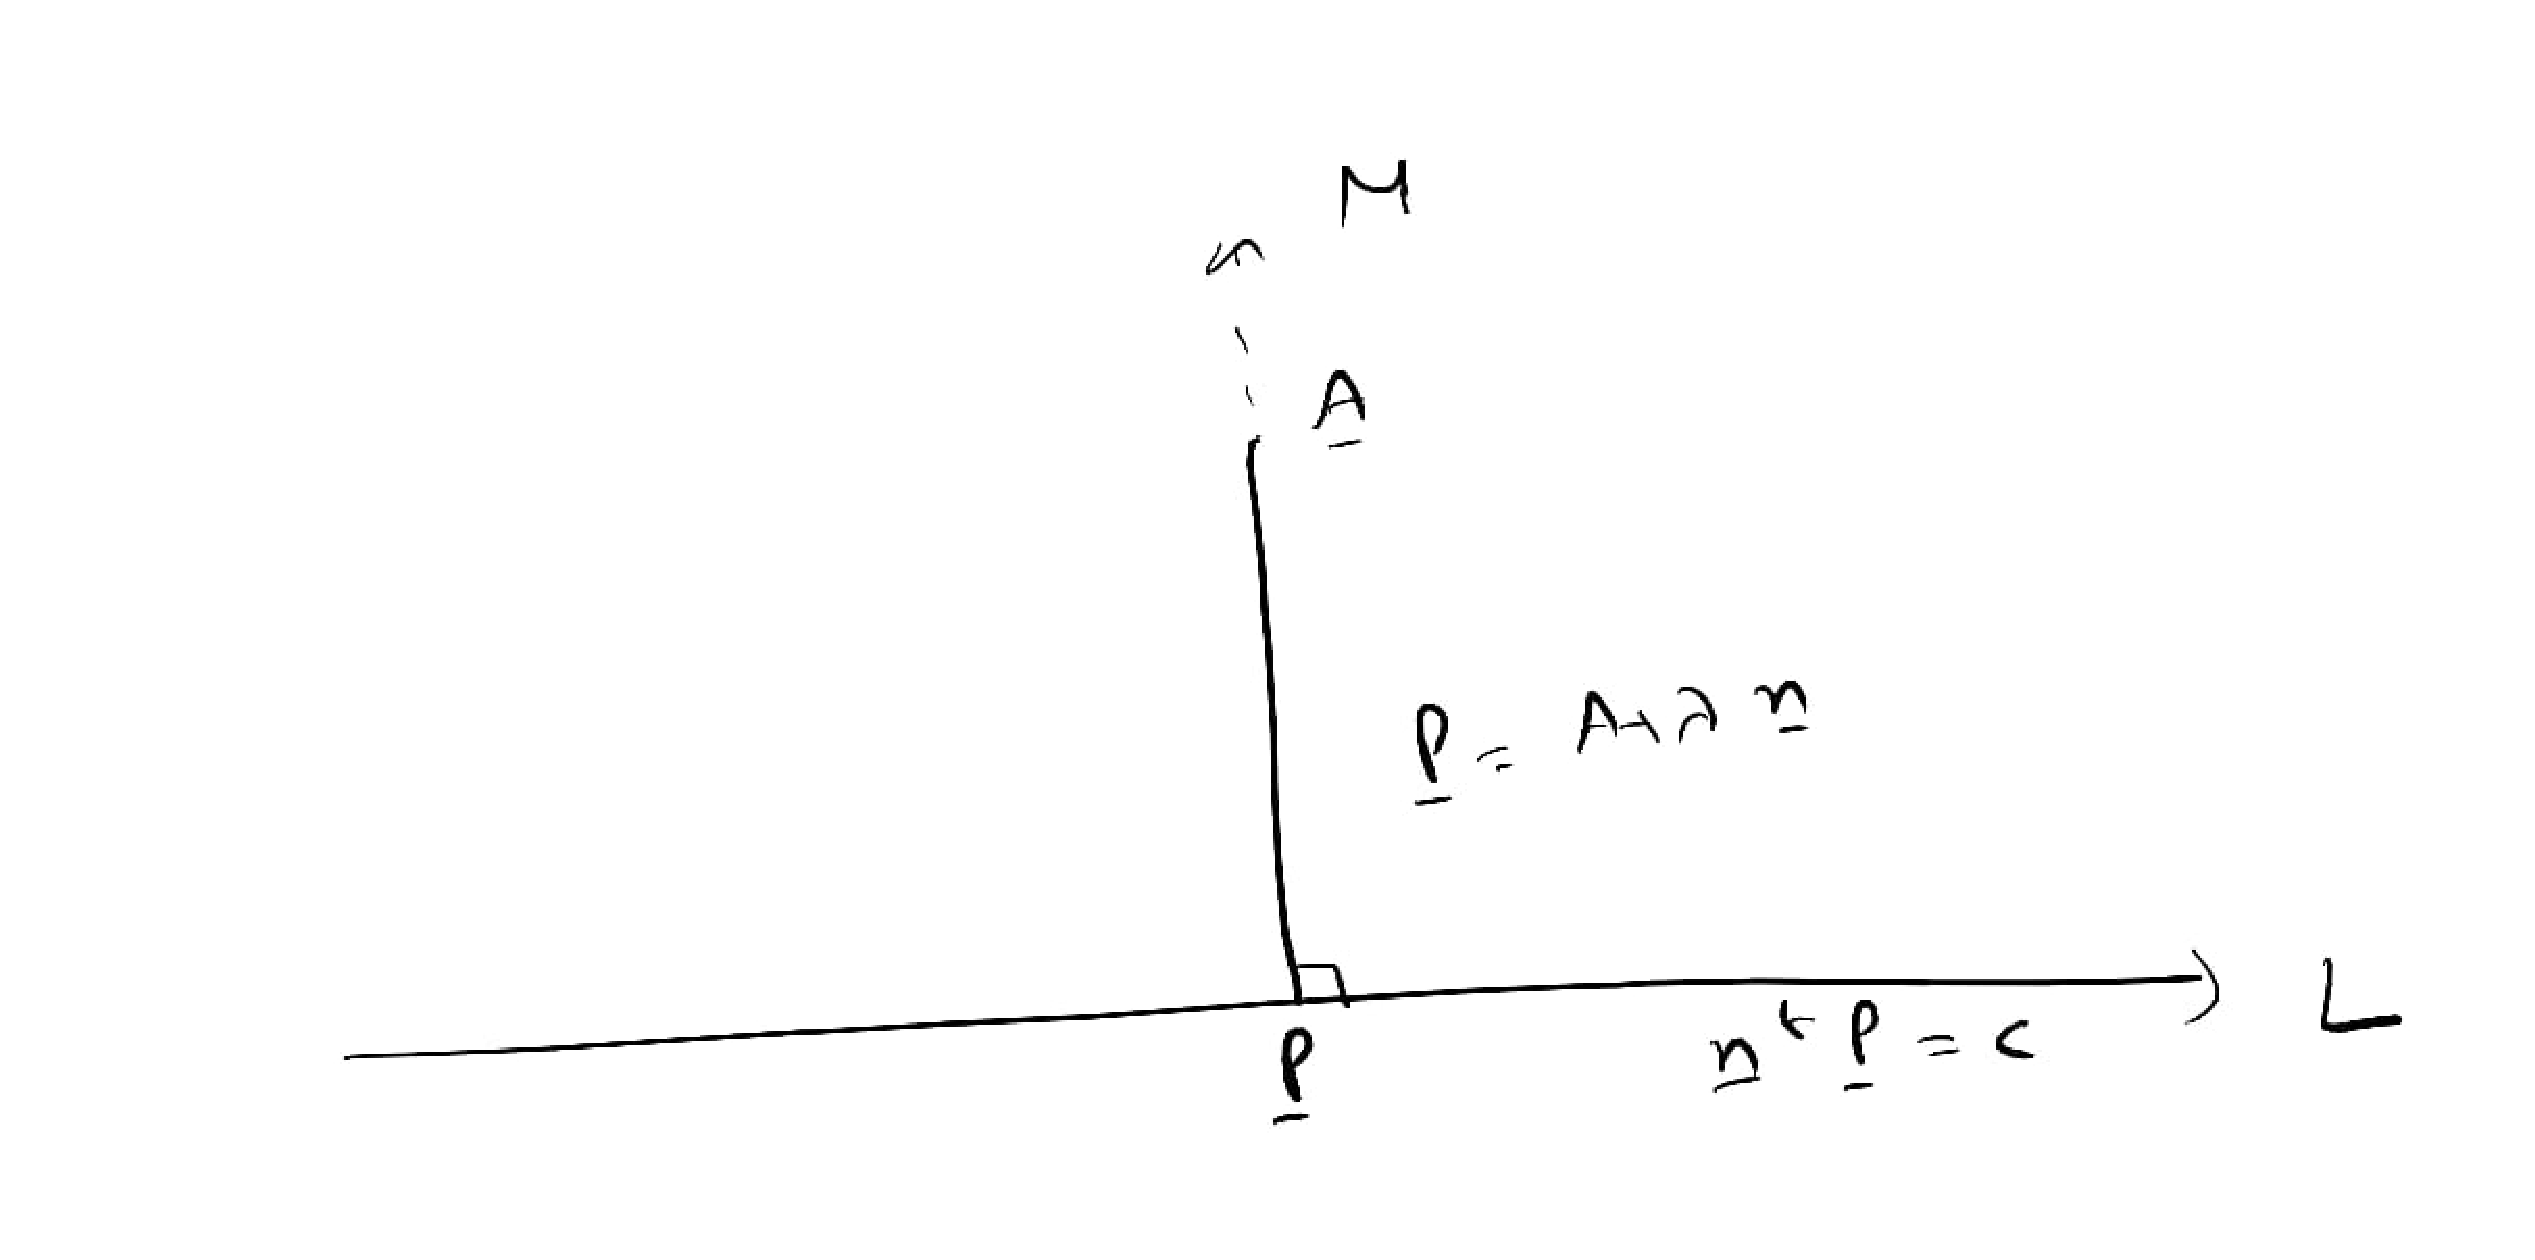
\includegraphics[width=\columnwidth]{./line/figs/line_pt_dist.eps}
\caption{}
\label{fig:line_pt_dist}
\end{figure}
%
\begin{align}
\vec{n} = \myvec{1\\\tan 15\degree}
\end{align}
%
$\because \vec{A} = \vec{0}$, 
\begin{align}
4 = \frac{\abs{ c}}{\norm{\vec{n}}} \implies c &= \pm 4\sqrt{1+\tan^2 15\degree} 
\\
&= \pm 4 \sec 15\degree
\end{align}
%
where 
%
\begin{align}
\sec \theta = \frac{1}{\cos \theta}
\end{align}
%
This follows from the fact that
%
\begin{align}
\cos^2 \theta + \sin^2 \theta &= 1
\\
\implies 1 + \frac{\sin^2 \theta}{\cos^2 \theta} &= \frac{1}{\cos^2 \theta}
\end{align}
%
It is easy to verify that 
%
\begin{align}
\frac{\sin \theta}{\cos \theta} &= \tan \theta
\\
\implies 1 + \tan^2 \theta &= \sec^2 \theta
\end{align}
%

Thus, the equation of the line is 
\begin{align}
\myvec{1 &\tan 15\degree} \vec{c} = \pm 4 \sec 15\degree
\end{align}
\item The Farenheit temperature $F$ and absolute temperature $K$ satisfy a linear equation.  Given $K=273$ when $F=32$ and that $K=373$  when $F=212$, express $K$ in terms of $F$ and find the value of $F$, when $K=0$.
%
\\
\solution Let 
\begin{align}
\vec{x}=\myvec{F & K} 
\end{align}
%
Since the relation between $F, K$ is linear, \myvec{273\\32}, \myvec{373\\21} are on a line.  The corresponding equation is obtained from \eqref{eq:line_norm_vec} and \eqref{eq:line_norm_dir} as 
%
\begin{align}
\myvec{11 & -100}\vec{x} &= \myvec{11 & -100}\myvec{273\\32} 
\\
\implies \myvec{11 & -100}\vec{x} &= -197
\end{align}
%
If \myvec{F\\0} is a point on the line, 
%
\begin{align}
\myvec{11 & -100}\myvec{F\\0} &= -197
\implies F = -\frac{197}{11}
\end{align}
%
\item Equation of a line is 
\begin{align}
\myvec{3 & – 4}\vec{x} + 10 = 0. 
\end{align}
Find its 
\begin{enumerate}
\item  slope, 
\item  x - and y-intercepts.
\end{enumerate}
%
\solution From the given information, 
%
\begin{align}
\vec{n} &= \myvec{3 \\ – 4}, 
\\
\vec{m} &= \myvec{4 \\ 3}, 
\end{align}
%
\begin{enumerate}
\item $m = \frac{3}{4}$
\item x-intercept is $-\frac{10}{3}$ and y-intercept is $\frac{10}{4} = \frac{5}{2}$.
\end{enumerate}
%
%
\item Find the angle between two vectors $\vec{a}$ and $\vec{b}$ where 
%
\begin{align}
\norm{\vec{a}} = 1,
\norm{\vec{b}} = 2,
\vec{a}^T\vec{b} = 1.
\end{align}
%
\solution In Fig. \ref{fig:line_scalar_prod}, from the cosine formula, 
%
\begin{align}
\cos \theta &= \frac{\norm{\vec{A}-\vec{B}}^2+\norm{\vec{B}-\vec{C}}^2-\norm{\vec{A}-\vec{C}}^2}{2\norm{\vec{A}-\vec{B}}\norm{\vec{B}-\vec{C}}}
\end{align}
Letting $\vec{a} = \vec{A}-\vec{B}, \vec{b} = \vec{B}-\vec{C}$, 
\begin{align}
\cos \theta &= \frac{\norm{\vec{a}}^2+\norm{\vec{b}}^2-\norm{\vec{a}+\vec{b}}^2}{2\norm{\vec{a}}\norm{\vec{b}}}
\\
&= \frac{\norm{\vec{a}}^2+\norm{\vec{b}}^2-\sbrak{\norm{\vec{a}}^2+\norm{\vec{b}}^2-2\vec{a}^T\vec{b}}}{2\norm{\vec{a}}\norm{\vec{b}}}
\\
\implies \cos \theta &=\frac{\vec{a}^T\vec{b}}{\norm{\vec{a}}\norm{\vec{b}}}
\end{align}
%
Thus, the angle $\theta$ between two vectors is given by 
%
\begin{align}
\label{eq:line_scalar_prod}
\cos \theta &= \frac{\vec{a}^T\vec{b}}{\norm{\vec{a}}\norm{\vec{b}}}
\\
&=\frac{1}{2}
\\
\implies \theta &= 60\degree
\end{align}
%
\begin{figure}[!ht]
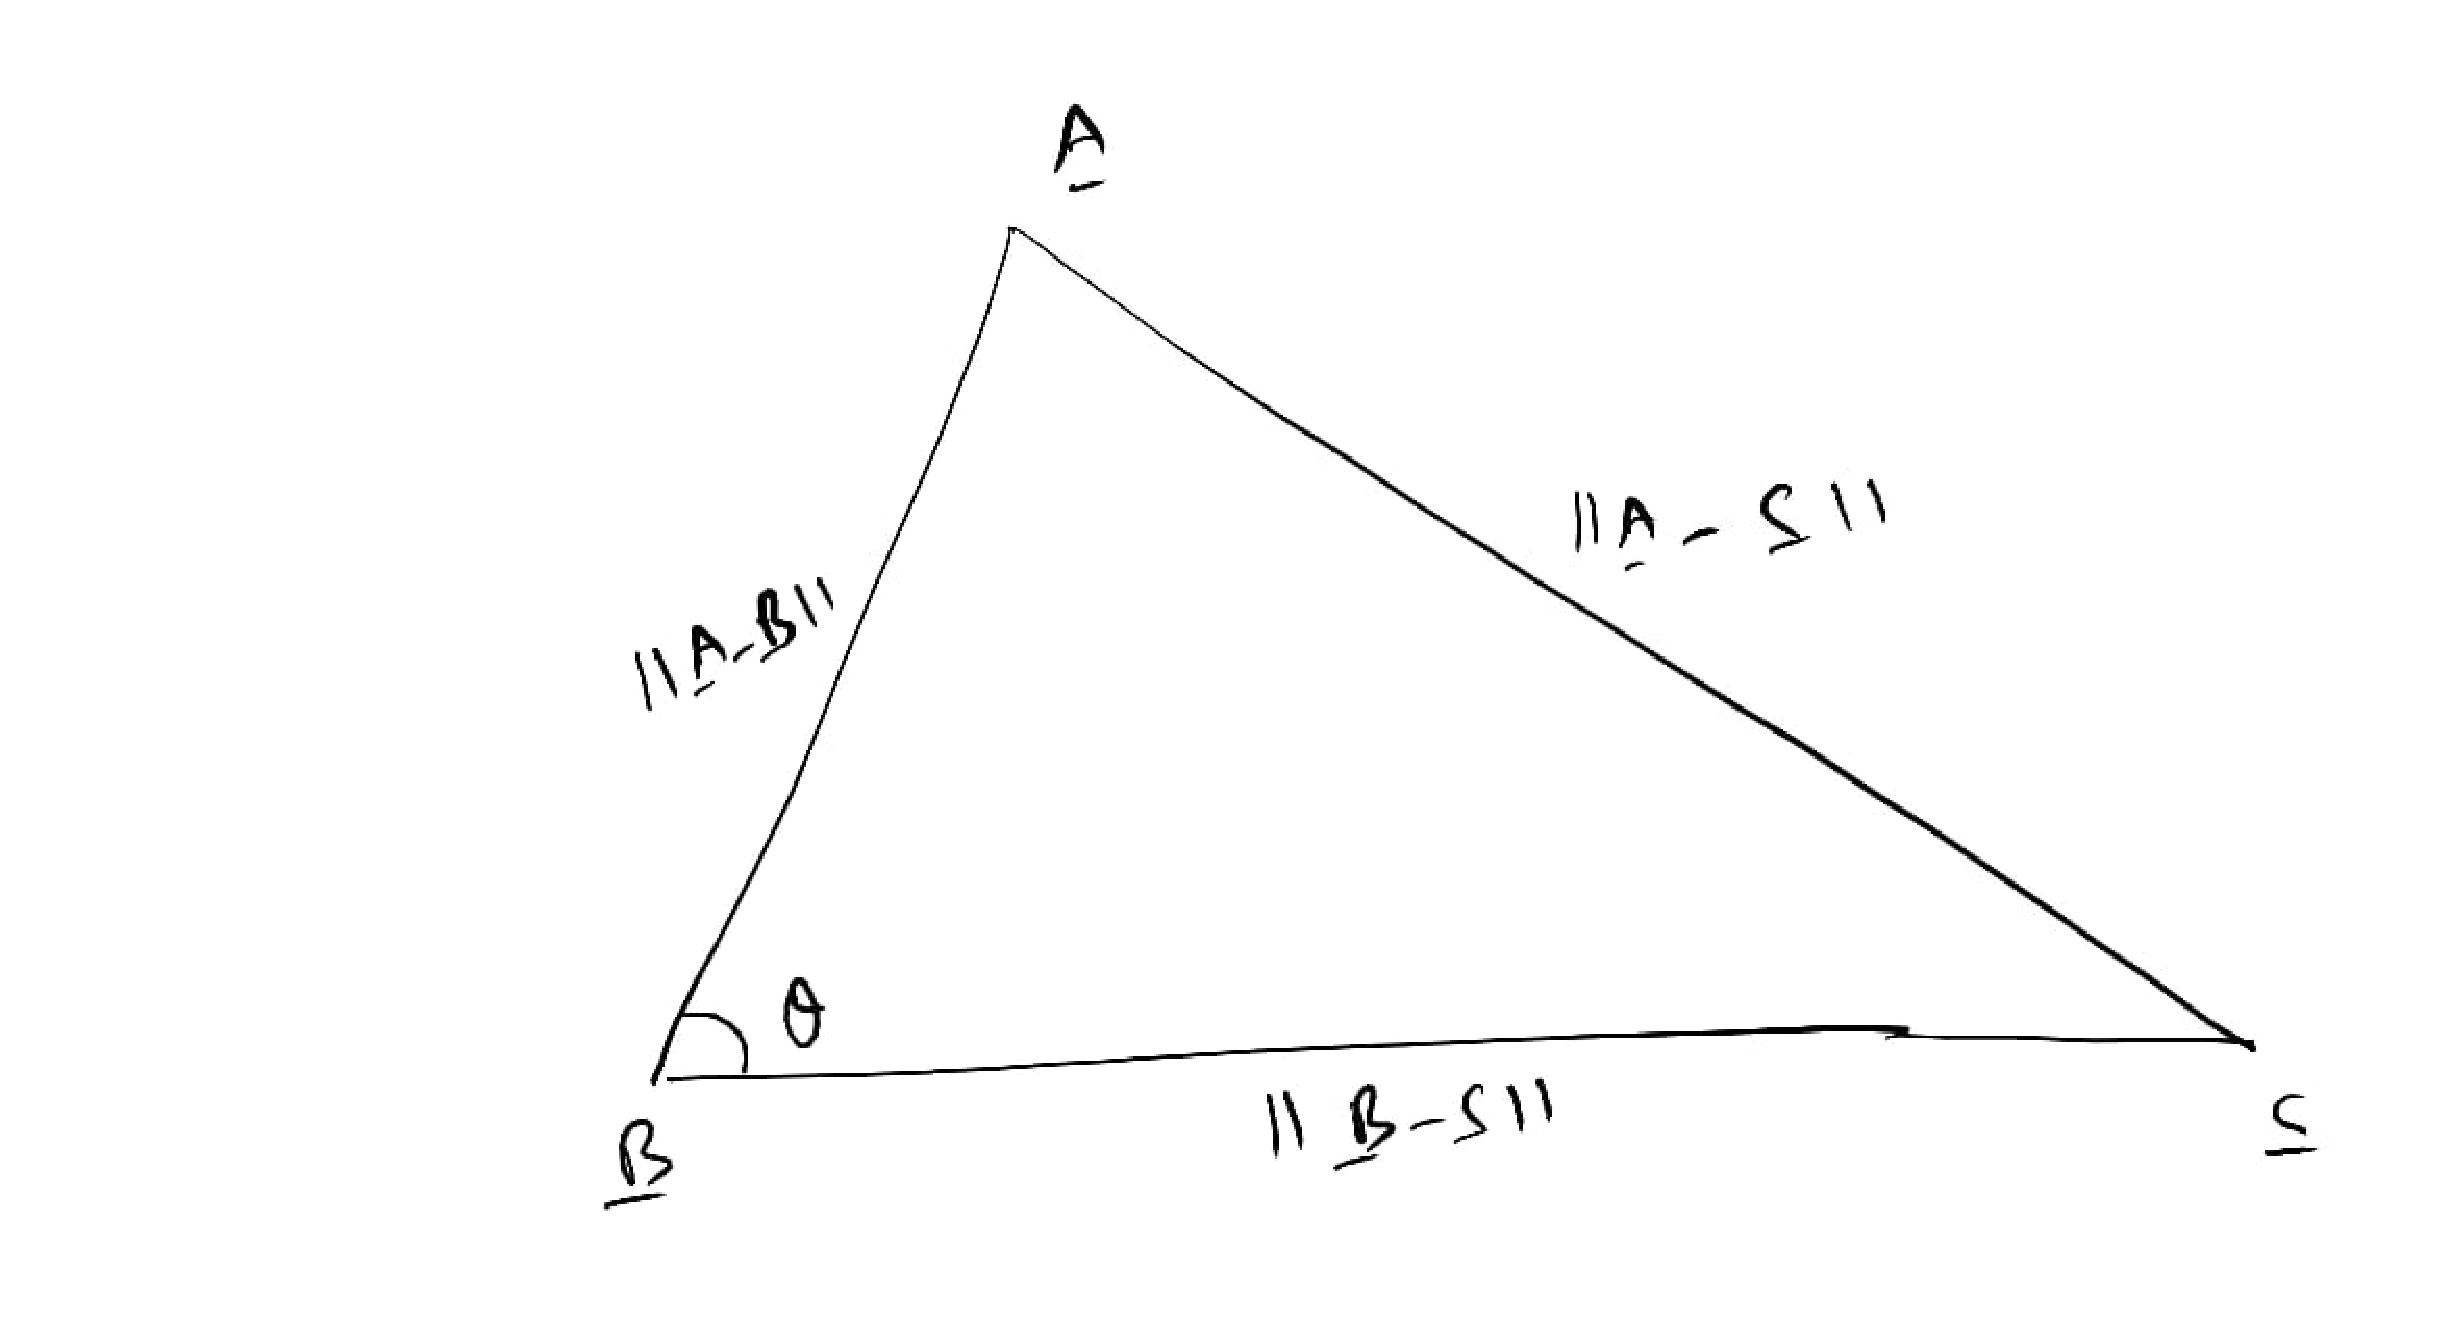
\includegraphics[width=\columnwidth]{./line/figs/line_scalar_prod.eps}
\caption{}
\label{fig:line_scalar_prod}
\end{figure}
%


\item Find the angle between the lines 
%
\begin{align}
\myvec{1 & – \sqrt{3}}\vec{x}  = 5
\\
\myvec{\sqrt{3} & –1}\vec{x}  = -6
. 
\end{align}
%
\solution The angle between the lines can also be expressed in terms of the normal vectors as
%
\begin{align}
\cos \theta &= \frac{\vec{n}_1\vec{n}_2}{\norm{\vec{n}_1}\norm{\vec{n}_2}}
\\
&= \frac{\sqrt{3}}{2} \implies \theta = 30\degree
\end{align}
%
\item Find the equation of a line perpendicular to the line 
\begin{align}
\myvec{1 & – 2}\vec{x}  = 3
\end{align}
%
and passes through the point \myvec{1\\-2}.
%
\\
\solution The normal vector of the perpendicular line is 
%
\begin{align}
\myvec{2 \\ 1}
\end{align}
%
Thus, the desired equation of the line is 
%
\begin{align}
\myvec{2 & 1}\brak{\vec{x} - \myvec{1\\-2}} &=0
\\
\implies \myvec{2 & 1}\vec{x} =0
\end{align}
%

\item Find the distance of the point \myvec{3\\-5} from the line 
\begin{align}
\myvec{3 & – 4}\vec{x}  = 26
\end{align}
%
\solution Use \eqref{eq:line_pt_dist}.

\item If the lines 
\begin{align}
\myvec{2 & 1}\vec{x}  = 3
\\
\myvec{5 & k}\vec{x}  = 3
\\
\myvec{3 & -1}\vec{x}  = 2
\end{align}
%
are concurrent, find the value of $k$.
%
\\
\solution If the lines are concurrent, the {\em augmented}  matrix should have a 0 row upon row reduction.  Hence, 
%
\begin{align}
\myvec{
2 & 1 & 3
\\
5 & k & 3
\\
3 & -1 & 2
}
\xleftrightarrow{R_2\leftrightarrow R_3}
\myvec{
2 & 1 & 3
\\
3 & -1 & 2
\\
5 & k & 3
}
\\
\xleftrightarrow [R_3\leftarrow 2R_3-5R_1]{R_2\leftrightarrow 2R_2-3R_1}
\myvec{
2 & 1 & 3
\\
0 & -5 & -5
\\
0 & 2k-5 & -9
}
\\
\xleftrightarrow []{R_2\leftarrow -\frac{R_2}{5}}
\myvec{
2 & 1 & 3
\\
0 & 1 & 1
\\
0 & 2k-5 & -9
}
\\
\xleftrightarrow []{R_3\leftarrow R_3-\brak{2k-5}R_2}
\myvec{
2 & 1 & 3
\\
0 & 1 & 1
\\
0 & 0 & -2k-4
}
\\
\implies k = -2
\end{align}
%
\item Find the distance of the line
\begin{align}
\label{eq:line_L_1}
L_1: \quad \myvec{4 & 1}\vec{x}  = 0
\end{align}
%
from the point \myvec{4\\1} measured along the line $L_2$ making an angle of $135\degree$ with the positive x-axis.
%
\\
\solution  Let $P$ be the point of intersection of $L_1$ and $L_2$.  The direction vector of $L_2$ is 
\begin{align}
\vec{m} = \myvec{1 \\ \tan 135\degree}
\end{align}
%
Since \myvec{4\\1} lies on $L_2$, the equation of $L_2$ is 
\begin{align}
\label{eq:line_L_2}
\vec{x} &= \myvec{4\\1} + \lambda \vec{m} 
\\
\label{eq:line_L_2_P}
\implies \vec{P} &= \myvec{4\\1} + \lambda \vec{m} 
\\
\label{eq:line_L_2_P_dist}
\text{or, } \norm{\vec{P} - \myvec{4\\1}} &= d = \abs{\lambda}\norm{\vec{m} }
%
\end{align}
%
Since $\vec{P}$ lies on $L_1$, from \eqref{eq:line_L_1},
%
\begin{align}
\myvec{4 & 1}\vec{P}  = 0
\end{align}
%
Substituting from the above in \eqref{eq:line_L_2},
%
\begin{align}
\myvec{4 & 1}\myvec{4\\1} + \lambda \myvec{4 & 1}\vec{m}  &= 0
\\
\implies \lambda &= \frac{\myvec{4 & 1}\vec{m}}{17}
\end{align}
%
substituting $\abs{\lambda}$ in \eqref{eq:line_L_2_P_dist} gives the desired answer.

\item Assuming that straight lines work as a plane mirror for a point, find the image of the point \myvec{1\\2} in the line 
%
\begin{align}
\myvec{1 & -3}\vec{x}  = -4.
\end{align}
%
%\item Find $\vec{R}$, the {\em reflection}  of $\vec{P}$ about the line
%\begin{align}
%L: \quad \vec{n}^T\vec{x} = c
%\end{align}
%
\begin{figure}
\centering
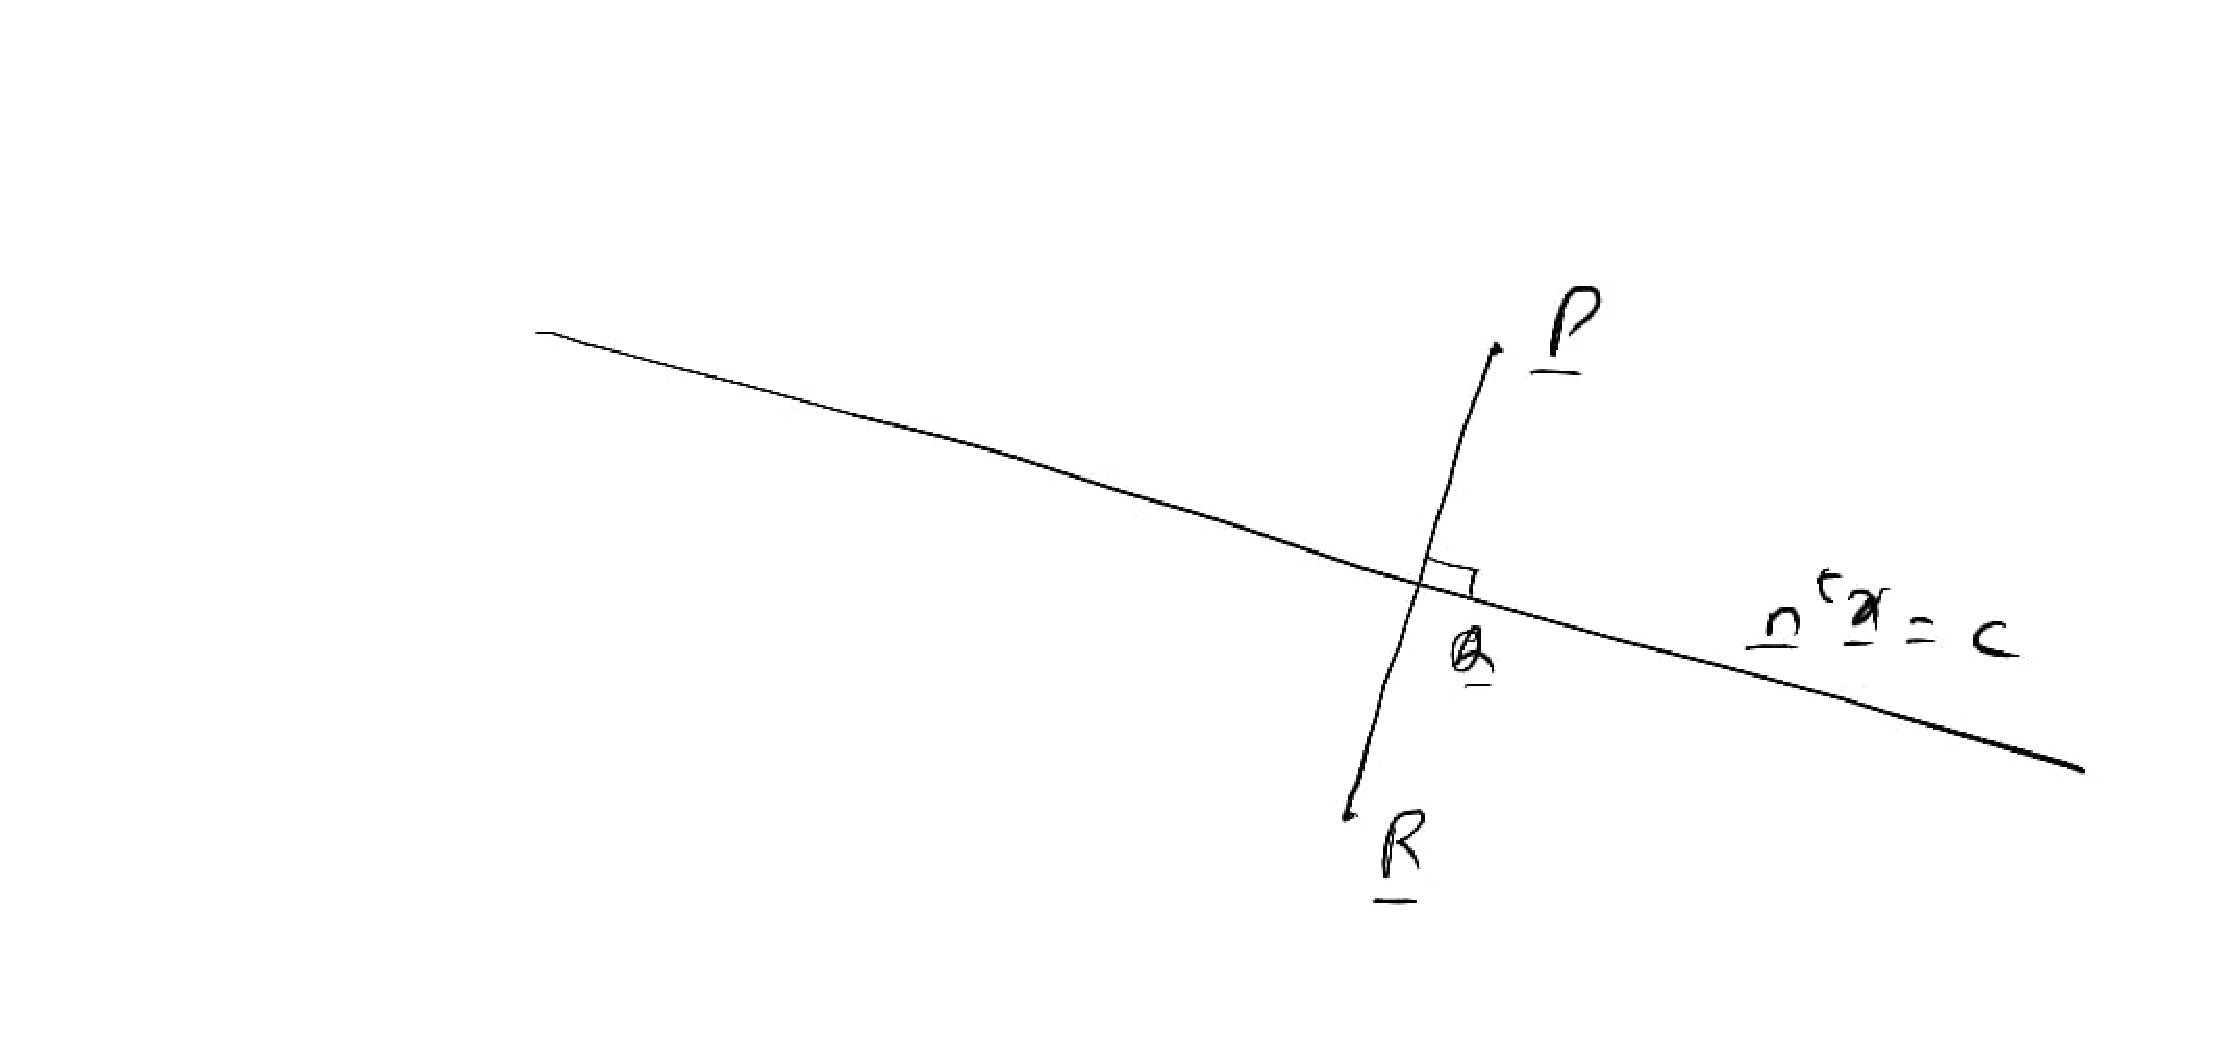
\includegraphics[width=\columnwidth]{./line/figs/reflection.eps}
\caption{}
\label{fig:line_reflection}
\end{figure}
\solution Since $\vec{R}$ is the reflection of $\vec{P}$ and $\vec{Q}$ lies on $L$, $\vec{Q}$ bisects $PR$.  
This leads to the following equations
\begin{align}
\label{eq:reflect_bisect}
2\vec{Q} &= \vec{P}+\vec{R}
\\
\label{eq:reflect_Q}
\vec{n}^{T}\vec{Q} &= c
\\
\label{eq:reflect_R}
\vec{m}^{T}\vec{R} &= \vec{m}^{T}\vec{P}
\end{align}
%
where $\vec{m}$ is the direction vector of $L$.  From \eqref{eq:reflect_bisect} and \eqref{eq:reflect_Q},
\begin{align}
\label{eq:reflect_bisectQ}
\vec{n}^{T}\vec{R}  &= 2c - \vec{n}^{T}\vec{P}
\end{align}
%
From \eqref{eq:reflect_bisectQ} and \eqref{eq:reflect_R},
\begin{align}
\label{eq:reflect_bisectQR}
\myvec{\vec{m} & \vec{n}}^T\vec{R} &= \myvec{\vec{m} & -\vec{n}}^T\vec{P}+ \myvec{0 \\ 2c}
\end{align}
%
Letting 
\begin{align}
\label{eq:reflect_mat}
\vec{V}=  \myvec{\vec{m} & \vec{n}}
\end{align}
with the condition that $\vec{m},\vec{n}$ are orthonormal, i.e.
\begin{align}
\label{eq:reflect_ortho}
\vec{V}^T\vec{V}=  \vec{I}
\end{align}
%
Noting that 
\begin{align}
\label{eq:reflect_trans}
\myvec{\vec{m} & -\vec{n}} &= \myvec{\vec{m} & \vec{n}} \myvec{1 & 0 \\ 0 & -1},
\end{align}
\eqref{eq:reflect_bisectQR} can be expressed as
%
\begin{align}
\label{eq:reflect_}
\vec{V}^T\vec{R} &=  \sbrak{\vec{V}\myvec{1 & 0 \\ 0 & -1}}^T\vec{P}+\myvec{0 \\ 2c}
\\
\implies \vec{R} &= \sbrak{\vec{V}\myvec{1 & 0 \\ 0 & -1}\vec{V}^{-1}}^T\vec{P}+ \vec{V}\myvec{0 \\ 2c}
\\
 &=\vec{V}\myvec{1 & 0 \\ 0 & -1}\vec{V}^T \vec{P}+2c \vec{n}
\end{align}
It can be verified that 
%\item Show that, for any $\vec{m},\vec{n}$, 
the reflection is also given by
\begin{align}
%\label{eq:reflect_bisect}
\frac{\vec{R}}{2} = \frac{\vec{m}\vec{m}^T-\vec{n}\vec{n}^T}{\vec{m}^T\vec{m}+\vec{n}^T\vec{n}}\vec{P} + c 
\frac{\vec{n}}{\norm{\vec{n}}^2}
\end{align}
%\solution The reflection of a point $\vec{P}$ about a line 
%%
%\begin{align}
%\vec{n}^T\vec{x}  = c
%\end{align}
%%
%is given by $\vec{R}$, where
%\begin{align}
%\label{eq:line_reflect}
%\frac{\vec{R}}{2} = \frac{\vec{m}\vec{m}^T-\vec{n}\vec{n}^T}{\vec{m}^T\vec{m}+\vec{n}^T\vec{n}}\vec{P} + c \frac{\vec{n}}{\norm{\vec{n}}^2}
%\end{align}
%
The following code plots Fig. \ref{fig:line_reflect} while computing the reflection
%
\begin{lstlisting}
codes/line/line_reflect.py
\end{lstlisting}
%
\begin{figure}[!ht]
\includegraphics[width=\columnwidth]{./line/figs/line_reflect.eps}
\caption{}
\label{fig:line_reflect}
\end{figure}
%

\item A line $L$ is such that its segment between the lines %
is bisected at the point $\vec{P} = \myvec{1\\5}$.  Obtain its equation.
\begin{align}
\label{eq:line_seg}
L_1: \quad \myvec{5 & -1}\vec{x}  &= -4
\\
L_2: \quad \myvec{3 & 4}\vec{x}  &= 4
\end{align}
%
\\
\solution Let 
%
\begin{align}
L: \quad \vec{x}  &= \vec{P} + \lambda \vec{m}
\end{align}
%
If $L$ intersects $L_1$ and $L_2$ at $\vec{A}$ and $\vec{B}$ respectively, 
%
\begin{align}
\label{eq:line_segA}
 \vec{A}  &= \vec{P} + \lambda \vec{m}
\\
 \vec{B}  &= \vec{P} - \lambda \vec{m}
\label{eq:line_segB}
\end{align}
%
since $\vec{P}$ bisects $AB$. Note that $\lambda$ is a measure of the distance from $P$  along the line $L$.
%
From \eqref{eq:line_seg}, \eqref{eq:line_segA} and \eqref{eq:line_segB},
%
\begin{align}
\myvec{5 & -1} \vec{A}  &= \myvec{5 & -1}\myvec{1\\5} + \lambda \myvec{5 & -1}\vec{m}=-4
\\
\myvec{3 & 4} \vec{B}  &= \myvec{3 & 4}\myvec{1\\5} - \lambda \myvec{3 & 4}\vec{m}=4
\end{align}
%
yielding
%
\begin{align}
19\myvec{5 & -1}\vec{m}&=-4 \myvec{3 & 4}\vec{m}
\\
\implies \myvec{107 & -3}\vec{m} &= 0
\\
\text{or, } \vec{n} = \myvec{107\\-3}
\end{align}
%
after simplification.
Thus, the equation of the line is 
\begin{align}
\vec{n}^T\brak{\vec{x}-\vec{P}} =0
\end{align}
\item Show that the path of a moving point such that its distances from two lines
%
\begin{align}
\myvec{3 & -2}\vec{x}  &= 5
\\
\myvec{3 & 2}\vec{x}  &= 5
\end{align}
%
are  equal is a straight line.
%
\\
\solution Using \eqref{eq:line_pt_dist} the point $\vec{x}$ satisfies
%
\begin{align}
\frac{\abs{\myvec{3 & -2}\vec{x}  - 5}}{\norm{\myvec{3 \\ -2}}}
&=\
\frac{\abs{\myvec{3 & 2}\vec{x}  - 5}}{\norm{\myvec{3 \\ 2}}}
\\
\implies \abs{\myvec{3 & -2}\vec{x}  - 5}&=\abs{\myvec{3 & 2}\vec{x}  - 5}
\end{align}
%
resulting in 
%
\begin{align}
\myvec{3 & -2}\vec{x}  - 5=\pm\brak{\myvec{3 & 2}\vec{x}  - 5}
\end{align}
%
leading to the possible lines
%
\begin{align}
L_1: \quad \myvec{0 & 1}\vec{x}  &=0
\\
L_2: \quad \myvec{1 & 0}\vec{x}  &=  \frac{5}{3}
\end{align}
%
\item Find the distance between the points
%
\begin{align}
\vec{P} = \myvec{1\\-3\\4},
\vec{Q} = \myvec{-4\\1\\2}
\end{align}
%
\solution 
\\
Let the balanced version of (\ref{eq:solutions/chem/6ato balance}) be
\begin{align}
    \label{eq:solutions/chem/6abalanced}x_{1}HNO_{3}+ x_{2}Ca(OH)_{2}\to x_{3}Ca(NO_{3})_{2}+ x_{4}H_{2}O
\end{align}

which results in the following equations:
\begin{align}
    (x_{1}+ 2x_{2}-2x_{4}) H= 0\\
    (x_{1}-2x_{3}) N= 0\\
    (3x_{1}+ 2x_{2}-6x_{3}- x_{4}) O=0\\
    (x_{2}-x_{3}) Ca= 0
\end{align}

which can be expressed as
\begin{align}
    x_{1}+ 2x_{2}+ 0.x_{3} -2x_{4} = 0\\
    x_{1}+ 0.x_{2} -2x_{3} +0.x_{4}= 0\\
    3x_{1}+ 2x_{2}-6x_{3}- x_{4} =0\\
    0.x_{1} +x_{2}-x_{3} +0.x_{4}= 0
\end{align}

resulting in the matrix equation
\begin{align}
    \label{eq:solutions/chem/6a matrix}
    \myvec{1 & 2 & 0 & -2\\
           1 & 0 & -2 & 0\\
           3 & 2 & -6 & -1\\
           0 & 1 & -1 & 0}\vec{x}
           =\vec{0}
\end{align}

where,
\begin{align}
   \vec{x}= \myvec{x_{1}\\x_{2}\\x_{3}\\x_{4}}
\end{align}

(\ref{eq:solutions/chem/6a matrix}) can be reduced as follows:
\begin{align}
    \myvec{1 & 2 & 0 & -2\\
           1 & 0 & -2 & 0\\
           3 & 2 & -6 & -1\\
           0 & 1 & -1 & 0}
    \xleftrightarrow[R_{3}\leftarrow \frac{R_3}{3}-R_{1}]{R_{2}\leftarrow R_2- R_1}
    \myvec{1 & 2 & 0 & -2\\
           0 & -2 & -2 & 2\\
           0 & -\frac{4}{3} & -2 & \frac{5}{3}\\
           0 & 1 & -1 & 0}\\
    \xleftrightarrow{R_2 \leftarrow -\frac{R_2}{2}}
    \myvec{1 & 2 & 0 & -2\\
          0 & 1 & 1 & -1\\
          0 & -\frac{4}{3} & -2 & \frac{5}{3}\\
          0 & 1 & -1 & 0}\\
    \xleftrightarrow[R_4 \leftarrow R_4- R_2]{R_3 \leftarrow R_3 + \frac{4}{3}R_2}
    \myvec{1 & 2 & 0 & -2\\
           0 & 1 & 1 & -1\\
           0 & 0 & -\frac{2}{3} & \frac{1}{3}\\
           0 & 0 & -2 & 1}\\
    \xleftrightarrow[R_3 \leftarrow -\frac{3}{2}R_3]{R_1 \leftarrow R_1- 2R_2}
    \myvec{1 & 0 & -2 & 0\\
           0 & 1 & 1 & -1\\
           0 & 0 & 1 & -\frac{1}{2}\\
           0 & 0 & -2 & 1}\\
    \xleftrightarrow{R_4\leftarrow R_4 + 2R_3}
    \myvec{1 & 0 & -2 & 0\\
           0 & 1 & 1 & -1\\
           0 & 0 & 1 & -\frac{1}{2}\\
           0 & 0 & 0 & 0}\\
    \xleftrightarrow[R_2\leftarrow R_2-R_3]{R_1\leftarrow R_1 + 2R_3}
    \myvec{1 & 0 & 0 & -1\\
           0 & 1 & 0 & -\frac{1}{2}\\
           0 & 0 & 1 & -\frac{1}{2}\\
           0 & 0 & 0 & 0}
\end{align}

Thus,
\begin{align}
    x_1=x_4, x_2= \frac{1}{2}x_4, x_3=\frac{1}{2}x_4\\
    \implies \quad\vec{x}= x_4\myvec{1\\ \frac{1}{2}\\ \frac{1}{2}\\1} =\myvec{2\\1\\1\\2}
\end{align} 
by substituting $x_4= 2$.

\hfill\break
%\vspace{5mm} 
Hence, (\ref{eq:solutions/chem/6abalanced}) finally becomes
\begin{align}
    2HNO_{3}+ Ca(OH)_{2}\to Ca(NO_{3})_{2}+ 2H_{2}O
\end{align}

The distance is given by $\norm{\vec{P}-\vec{Q}}$
\item Show that the points 
\label{prob:line_coll_3d}
$
\vec{A}=\myvec{-2\\3\\5}, 
\vec{B}=\myvec{1\\2\\3}$ 
and 
$ \vec{C}=\myvec{7\\0\\-1}$ 
are collinear.
%
\\
\solution Forming the matrix in \eqref{eq:tri_geo_ex_diff_mat}
%
\begin{align}
\vec{M} = \myvec{
3 & -1 & -2
\\
9 & -3 & -6
}
\xleftrightarrow {R_2\leftarrow R_2-3R_1}
\myvec{
3 & -1 & -2
\\
0 & 0 & 0
}
\end{align}
%
$\implies rank(\vec{M}) = 1$.
%
The following code plots Fig. \ref{fig:collinear_3d} showing that the points are collinear.
%
\begin{lstlisting}
codes/line/draw_lines_3d.py
\end{lstlisting}
%
\begin{figure}[!ht]
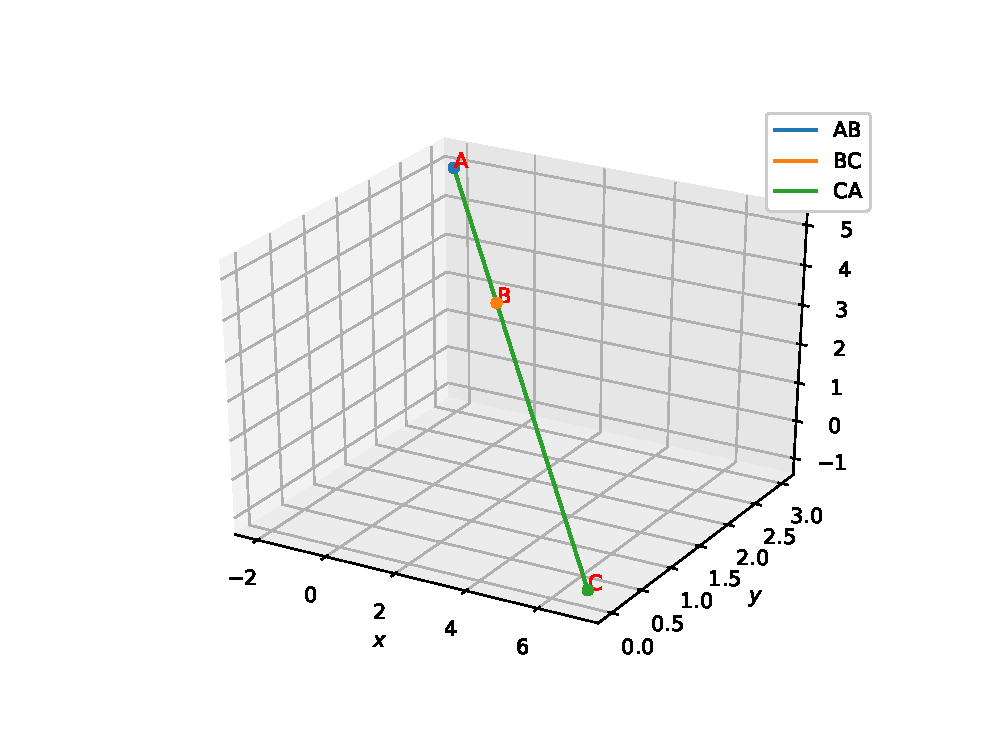
\includegraphics[width=\columnwidth]{./line/figs/collinear_3d.eps}
\caption{}
\label{fig:collinear_3d}
\end{figure}
%
\item Show that 
$
\vec{A}=\myvec{2\\3\\-4}, 
\vec{B}=\myvec{1\\-2\\3} \text{ and } 
\vec{C}=\myvec{3\\8\\-11}$  
are collinear.
%
\\
\solution Use the approach in Problem \eqref{prob:line_coll_3d}.
%
\item Find the equation of set of points $\vec{P}$ such that
\begin{align}
PA^2+PB^2 =2k^2,
\end{align}
%
\begin{align}
\vec{A} = \myvec{3\\4 \\5},
\vec{B} = \myvec{-1\\3 \\-7},
\end{align}
%
respectively.
%
\item Find the coordinates of a point which divides the line segment joining the points \myvec{1\\-2\\3} and \myvec{3\\4\\-5} in the ratio $2:3$
\begin{enumerate}
\item internally, and
\item externally.
\end{enumerate}
%
\solution Use \eqref{eq:line_section_form}.

\item Prove that the three points \myvec{-4\\6\\10}, \myvec{2\\4\\6} and \myvec{14\\0\\-2} are collinear.
%
\\
\solution  Use the approach in Problem \ref{prob:line_coll_3d}.
%
\item Find the ratio in which the line segment joining the points \myvec{4\\8\\10} and \myvec{6\\10\\-8} is divided by the YZ-plane.
%
\\
\solution Use \eqref{eq:line_section_form}.  The YZ-plane has points \myvec{0\\y\\z}.
%
\item Find the equation of the set of points $\vec{P}$ such that its distances from the points
$
\vec{A}=\myvec{3\\4\\-5}, 
\vec{B}=\myvec{-2\\1\\4}
$
are equal. 
%
\\
\solution Use the approach in Problem \ref{prob:line_perp_bisect}.
\item If 
\begin{align}
\vec{P} = 3\vec{a}-2\vec{b}
\\
\vec{Q} = \vec{a}+\vec{b}
\end{align}
%
find $\vec{R}$, which divides $PQ$ in the ratio $2:1$
\begin{enumerate}
\item internally,
\item externally.
\end{enumerate}
%
\solution Use \eqref{eq:line_section_form}.  
\item Find the angle between the vectors 
$\vec{a}=\myvec{1\\1\\-1}$
  and 
$\vec{b}=\myvec{1\\-1\\1}$.
%
\\
\solution 
Let the balanced version of (\ref{eq:solutions/chem/6ato balance}) be
\begin{align}
    \label{eq:solutions/chem/6abalanced}x_{1}HNO_{3}+ x_{2}Ca(OH)_{2}\to x_{3}Ca(NO_{3})_{2}+ x_{4}H_{2}O
\end{align}

which results in the following equations:
\begin{align}
    (x_{1}+ 2x_{2}-2x_{4}) H= 0\\
    (x_{1}-2x_{3}) N= 0\\
    (3x_{1}+ 2x_{2}-6x_{3}- x_{4}) O=0\\
    (x_{2}-x_{3}) Ca= 0
\end{align}

which can be expressed as
\begin{align}
    x_{1}+ 2x_{2}+ 0.x_{3} -2x_{4} = 0\\
    x_{1}+ 0.x_{2} -2x_{3} +0.x_{4}= 0\\
    3x_{1}+ 2x_{2}-6x_{3}- x_{4} =0\\
    0.x_{1} +x_{2}-x_{3} +0.x_{4}= 0
\end{align}

resulting in the matrix equation
\begin{align}
    \label{eq:solutions/chem/6a matrix}
    \myvec{1 & 2 & 0 & -2\\
           1 & 0 & -2 & 0\\
           3 & 2 & -6 & -1\\
           0 & 1 & -1 & 0}\vec{x}
           =\vec{0}
\end{align}

where,
\begin{align}
   \vec{x}= \myvec{x_{1}\\x_{2}\\x_{3}\\x_{4}}
\end{align}

(\ref{eq:solutions/chem/6a matrix}) can be reduced as follows:
\begin{align}
    \myvec{1 & 2 & 0 & -2\\
           1 & 0 & -2 & 0\\
           3 & 2 & -6 & -1\\
           0 & 1 & -1 & 0}
    \xleftrightarrow[R_{3}\leftarrow \frac{R_3}{3}-R_{1}]{R_{2}\leftarrow R_2- R_1}
    \myvec{1 & 2 & 0 & -2\\
           0 & -2 & -2 & 2\\
           0 & -\frac{4}{3} & -2 & \frac{5}{3}\\
           0 & 1 & -1 & 0}\\
    \xleftrightarrow{R_2 \leftarrow -\frac{R_2}{2}}
    \myvec{1 & 2 & 0 & -2\\
          0 & 1 & 1 & -1\\
          0 & -\frac{4}{3} & -2 & \frac{5}{3}\\
          0 & 1 & -1 & 0}\\
    \xleftrightarrow[R_4 \leftarrow R_4- R_2]{R_3 \leftarrow R_3 + \frac{4}{3}R_2}
    \myvec{1 & 2 & 0 & -2\\
           0 & 1 & 1 & -1\\
           0 & 0 & -\frac{2}{3} & \frac{1}{3}\\
           0 & 0 & -2 & 1}\\
    \xleftrightarrow[R_3 \leftarrow -\frac{3}{2}R_3]{R_1 \leftarrow R_1- 2R_2}
    \myvec{1 & 0 & -2 & 0\\
           0 & 1 & 1 & -1\\
           0 & 0 & 1 & -\frac{1}{2}\\
           0 & 0 & -2 & 1}\\
    \xleftrightarrow{R_4\leftarrow R_4 + 2R_3}
    \myvec{1 & 0 & -2 & 0\\
           0 & 1 & 1 & -1\\
           0 & 0 & 1 & -\frac{1}{2}\\
           0 & 0 & 0 & 0}\\
    \xleftrightarrow[R_2\leftarrow R_2-R_3]{R_1\leftarrow R_1 + 2R_3}
    \myvec{1 & 0 & 0 & -1\\
           0 & 1 & 0 & -\frac{1}{2}\\
           0 & 0 & 1 & -\frac{1}{2}\\
           0 & 0 & 0 & 0}
\end{align}

Thus,
\begin{align}
    x_1=x_4, x_2= \frac{1}{2}x_4, x_3=\frac{1}{2}x_4\\
    \implies \quad\vec{x}= x_4\myvec{1\\ \frac{1}{2}\\ \frac{1}{2}\\1} =\myvec{2\\1\\1\\2}
\end{align} 
by substituting $x_4= 2$.

\hfill\break
%\vspace{5mm} 
Hence, (\ref{eq:solutions/chem/6abalanced}) finally becomes
\begin{align}
    2HNO_{3}+ Ca(OH)_{2}\to Ca(NO_{3})_{2}+ 2H_{2}O
\end{align}

%
\item Find the angle between the pair of lines given by 
\begin{align}
\vec{x} &= \myvec{3\\2\\-4} + \lambda_1\myvec{1 \\ 2 \\2}
\\
\vec{x} &= \myvec{5\\-2\\0} + \lambda_2\myvec{3 \\ 2 \\6}
\end{align}
%
\\
\solution 
Let the balanced version of (\ref{eq:solutions/chem/6ato balance}) be
\begin{align}
    \label{eq:solutions/chem/6abalanced}x_{1}HNO_{3}+ x_{2}Ca(OH)_{2}\to x_{3}Ca(NO_{3})_{2}+ x_{4}H_{2}O
\end{align}

which results in the following equations:
\begin{align}
    (x_{1}+ 2x_{2}-2x_{4}) H= 0\\
    (x_{1}-2x_{3}) N= 0\\
    (3x_{1}+ 2x_{2}-6x_{3}- x_{4}) O=0\\
    (x_{2}-x_{3}) Ca= 0
\end{align}

which can be expressed as
\begin{align}
    x_{1}+ 2x_{2}+ 0.x_{3} -2x_{4} = 0\\
    x_{1}+ 0.x_{2} -2x_{3} +0.x_{4}= 0\\
    3x_{1}+ 2x_{2}-6x_{3}- x_{4} =0\\
    0.x_{1} +x_{2}-x_{3} +0.x_{4}= 0
\end{align}

resulting in the matrix equation
\begin{align}
    \label{eq:solutions/chem/6a matrix}
    \myvec{1 & 2 & 0 & -2\\
           1 & 0 & -2 & 0\\
           3 & 2 & -6 & -1\\
           0 & 1 & -1 & 0}\vec{x}
           =\vec{0}
\end{align}

where,
\begin{align}
   \vec{x}= \myvec{x_{1}\\x_{2}\\x_{3}\\x_{4}}
\end{align}

(\ref{eq:solutions/chem/6a matrix}) can be reduced as follows:
\begin{align}
    \myvec{1 & 2 & 0 & -2\\
           1 & 0 & -2 & 0\\
           3 & 2 & -6 & -1\\
           0 & 1 & -1 & 0}
    \xleftrightarrow[R_{3}\leftarrow \frac{R_3}{3}-R_{1}]{R_{2}\leftarrow R_2- R_1}
    \myvec{1 & 2 & 0 & -2\\
           0 & -2 & -2 & 2\\
           0 & -\frac{4}{3} & -2 & \frac{5}{3}\\
           0 & 1 & -1 & 0}\\
    \xleftrightarrow{R_2 \leftarrow -\frac{R_2}{2}}
    \myvec{1 & 2 & 0 & -2\\
          0 & 1 & 1 & -1\\
          0 & -\frac{4}{3} & -2 & \frac{5}{3}\\
          0 & 1 & -1 & 0}\\
    \xleftrightarrow[R_4 \leftarrow R_4- R_2]{R_3 \leftarrow R_3 + \frac{4}{3}R_2}
    \myvec{1 & 2 & 0 & -2\\
           0 & 1 & 1 & -1\\
           0 & 0 & -\frac{2}{3} & \frac{1}{3}\\
           0 & 0 & -2 & 1}\\
    \xleftrightarrow[R_3 \leftarrow -\frac{3}{2}R_3]{R_1 \leftarrow R_1- 2R_2}
    \myvec{1 & 0 & -2 & 0\\
           0 & 1 & 1 & -1\\
           0 & 0 & 1 & -\frac{1}{2}\\
           0 & 0 & -2 & 1}\\
    \xleftrightarrow{R_4\leftarrow R_4 + 2R_3}
    \myvec{1 & 0 & -2 & 0\\
           0 & 1 & 1 & -1\\
           0 & 0 & 1 & -\frac{1}{2}\\
           0 & 0 & 0 & 0}\\
    \xleftrightarrow[R_2\leftarrow R_2-R_3]{R_1\leftarrow R_1 + 2R_3}
    \myvec{1 & 0 & 0 & -1\\
           0 & 1 & 0 & -\frac{1}{2}\\
           0 & 0 & 1 & -\frac{1}{2}\\
           0 & 0 & 0 & 0}
\end{align}

Thus,
\begin{align}
    x_1=x_4, x_2= \frac{1}{2}x_4, x_3=\frac{1}{2}x_4\\
    \implies \quad\vec{x}= x_4\myvec{1\\ \frac{1}{2}\\ \frac{1}{2}\\1} =\myvec{2\\1\\1\\2}
\end{align} 
by substituting $x_4= 2$.

\hfill\break
%\vspace{5mm} 
Hence, (\ref{eq:solutions/chem/6abalanced}) finally becomes
\begin{align}
    2HNO_{3}+ Ca(OH)_{2}\to Ca(NO_{3})_{2}+ 2H_{2}O
\end{align}

\item Find the angle between the pair of lines
\begin{align}
\frac{x+3}{3} = \frac{y-1}{5} &= \frac{z+3}{4}, 
\\
\frac{x+1}{1} = \frac{y-4}{1} &= \frac{z-5}{2} 
\end{align}
%
\\
\solution 
Let the balanced version of (\ref{eq:solutions/chem/6ato balance}) be
\begin{align}
    \label{eq:solutions/chem/6abalanced}x_{1}HNO_{3}+ x_{2}Ca(OH)_{2}\to x_{3}Ca(NO_{3})_{2}+ x_{4}H_{2}O
\end{align}

which results in the following equations:
\begin{align}
    (x_{1}+ 2x_{2}-2x_{4}) H= 0\\
    (x_{1}-2x_{3}) N= 0\\
    (3x_{1}+ 2x_{2}-6x_{3}- x_{4}) O=0\\
    (x_{2}-x_{3}) Ca= 0
\end{align}

which can be expressed as
\begin{align}
    x_{1}+ 2x_{2}+ 0.x_{3} -2x_{4} = 0\\
    x_{1}+ 0.x_{2} -2x_{3} +0.x_{4}= 0\\
    3x_{1}+ 2x_{2}-6x_{3}- x_{4} =0\\
    0.x_{1} +x_{2}-x_{3} +0.x_{4}= 0
\end{align}

resulting in the matrix equation
\begin{align}
    \label{eq:solutions/chem/6a matrix}
    \myvec{1 & 2 & 0 & -2\\
           1 & 0 & -2 & 0\\
           3 & 2 & -6 & -1\\
           0 & 1 & -1 & 0}\vec{x}
           =\vec{0}
\end{align}

where,
\begin{align}
   \vec{x}= \myvec{x_{1}\\x_{2}\\x_{3}\\x_{4}}
\end{align}

(\ref{eq:solutions/chem/6a matrix}) can be reduced as follows:
\begin{align}
    \myvec{1 & 2 & 0 & -2\\
           1 & 0 & -2 & 0\\
           3 & 2 & -6 & -1\\
           0 & 1 & -1 & 0}
    \xleftrightarrow[R_{3}\leftarrow \frac{R_3}{3}-R_{1}]{R_{2}\leftarrow R_2- R_1}
    \myvec{1 & 2 & 0 & -2\\
           0 & -2 & -2 & 2\\
           0 & -\frac{4}{3} & -2 & \frac{5}{3}\\
           0 & 1 & -1 & 0}\\
    \xleftrightarrow{R_2 \leftarrow -\frac{R_2}{2}}
    \myvec{1 & 2 & 0 & -2\\
          0 & 1 & 1 & -1\\
          0 & -\frac{4}{3} & -2 & \frac{5}{3}\\
          0 & 1 & -1 & 0}\\
    \xleftrightarrow[R_4 \leftarrow R_4- R_2]{R_3 \leftarrow R_3 + \frac{4}{3}R_2}
    \myvec{1 & 2 & 0 & -2\\
           0 & 1 & 1 & -1\\
           0 & 0 & -\frac{2}{3} & \frac{1}{3}\\
           0 & 0 & -2 & 1}\\
    \xleftrightarrow[R_3 \leftarrow -\frac{3}{2}R_3]{R_1 \leftarrow R_1- 2R_2}
    \myvec{1 & 0 & -2 & 0\\
           0 & 1 & 1 & -1\\
           0 & 0 & 1 & -\frac{1}{2}\\
           0 & 0 & -2 & 1}\\
    \xleftrightarrow{R_4\leftarrow R_4 + 2R_3}
    \myvec{1 & 0 & -2 & 0\\
           0 & 1 & 1 & -1\\
           0 & 0 & 1 & -\frac{1}{2}\\
           0 & 0 & 0 & 0}\\
    \xleftrightarrow[R_2\leftarrow R_2-R_3]{R_1\leftarrow R_1 + 2R_3}
    \myvec{1 & 0 & 0 & -1\\
           0 & 1 & 0 & -\frac{1}{2}\\
           0 & 0 & 1 & -\frac{1}{2}\\
           0 & 0 & 0 & 0}
\end{align}

Thus,
\begin{align}
    x_1=x_4, x_2= \frac{1}{2}x_4, x_3=\frac{1}{2}x_4\\
    \implies \quad\vec{x}= x_4\myvec{1\\ \frac{1}{2}\\ \frac{1}{2}\\1} =\myvec{2\\1\\1\\2}
\end{align} 
by substituting $x_4= 2$.

\hfill\break
%\vspace{5mm} 
Hence, (\ref{eq:solutions/chem/6abalanced}) finally becomes
\begin{align}
    2HNO_{3}+ Ca(OH)_{2}\to Ca(NO_{3})_{2}+ 2H_{2}O
\end{align}

%
\item If 
$\vec{a}=\myvec{5\\-1\\-3}$
  and 
$\vec{b}=\myvec{1\\3\\-5}$,
%
then show that the vectors $\vec{a}+\vec{b}$ and $\vec{a}-\vec{b}$ are perpendicular.
%
\\
\solution 
Let the balanced version of (\ref{eq:solutions/chem/6ato balance}) be
\begin{align}
    \label{eq:solutions/chem/6abalanced}x_{1}HNO_{3}+ x_{2}Ca(OH)_{2}\to x_{3}Ca(NO_{3})_{2}+ x_{4}H_{2}O
\end{align}

which results in the following equations:
\begin{align}
    (x_{1}+ 2x_{2}-2x_{4}) H= 0\\
    (x_{1}-2x_{3}) N= 0\\
    (3x_{1}+ 2x_{2}-6x_{3}- x_{4}) O=0\\
    (x_{2}-x_{3}) Ca= 0
\end{align}

which can be expressed as
\begin{align}
    x_{1}+ 2x_{2}+ 0.x_{3} -2x_{4} = 0\\
    x_{1}+ 0.x_{2} -2x_{3} +0.x_{4}= 0\\
    3x_{1}+ 2x_{2}-6x_{3}- x_{4} =0\\
    0.x_{1} +x_{2}-x_{3} +0.x_{4}= 0
\end{align}

resulting in the matrix equation
\begin{align}
    \label{eq:solutions/chem/6a matrix}
    \myvec{1 & 2 & 0 & -2\\
           1 & 0 & -2 & 0\\
           3 & 2 & -6 & -1\\
           0 & 1 & -1 & 0}\vec{x}
           =\vec{0}
\end{align}

where,
\begin{align}
   \vec{x}= \myvec{x_{1}\\x_{2}\\x_{3}\\x_{4}}
\end{align}

(\ref{eq:solutions/chem/6a matrix}) can be reduced as follows:
\begin{align}
    \myvec{1 & 2 & 0 & -2\\
           1 & 0 & -2 & 0\\
           3 & 2 & -6 & -1\\
           0 & 1 & -1 & 0}
    \xleftrightarrow[R_{3}\leftarrow \frac{R_3}{3}-R_{1}]{R_{2}\leftarrow R_2- R_1}
    \myvec{1 & 2 & 0 & -2\\
           0 & -2 & -2 & 2\\
           0 & -\frac{4}{3} & -2 & \frac{5}{3}\\
           0 & 1 & -1 & 0}\\
    \xleftrightarrow{R_2 \leftarrow -\frac{R_2}{2}}
    \myvec{1 & 2 & 0 & -2\\
          0 & 1 & 1 & -1\\
          0 & -\frac{4}{3} & -2 & \frac{5}{3}\\
          0 & 1 & -1 & 0}\\
    \xleftrightarrow[R_4 \leftarrow R_4- R_2]{R_3 \leftarrow R_3 + \frac{4}{3}R_2}
    \myvec{1 & 2 & 0 & -2\\
           0 & 1 & 1 & -1\\
           0 & 0 & -\frac{2}{3} & \frac{1}{3}\\
           0 & 0 & -2 & 1}\\
    \xleftrightarrow[R_3 \leftarrow -\frac{3}{2}R_3]{R_1 \leftarrow R_1- 2R_2}
    \myvec{1 & 0 & -2 & 0\\
           0 & 1 & 1 & -1\\
           0 & 0 & 1 & -\frac{1}{2}\\
           0 & 0 & -2 & 1}\\
    \xleftrightarrow{R_4\leftarrow R_4 + 2R_3}
    \myvec{1 & 0 & -2 & 0\\
           0 & 1 & 1 & -1\\
           0 & 0 & 1 & -\frac{1}{2}\\
           0 & 0 & 0 & 0}\\
    \xleftrightarrow[R_2\leftarrow R_2-R_3]{R_1\leftarrow R_1 + 2R_3}
    \myvec{1 & 0 & 0 & -1\\
           0 & 1 & 0 & -\frac{1}{2}\\
           0 & 0 & 1 & -\frac{1}{2}\\
           0 & 0 & 0 & 0}
\end{align}

Thus,
\begin{align}
    x_1=x_4, x_2= \frac{1}{2}x_4, x_3=\frac{1}{2}x_4\\
    \implies \quad\vec{x}= x_4\myvec{1\\ \frac{1}{2}\\ \frac{1}{2}\\1} =\myvec{2\\1\\1\\2}
\end{align} 
by substituting $x_4= 2$.

\hfill\break
%\vspace{5mm} 
Hence, (\ref{eq:solutions/chem/6abalanced}) finally becomes
\begin{align}
    2HNO_{3}+ Ca(OH)_{2}\to Ca(NO_{3})_{2}+ 2H_{2}O
\end{align}

%

\item Find the projection of the vector 
\begin{align}
\vec{a} = \myvec{2\\3\\2}
\end{align}
on the vector
\begin{align}
\vec{b}=\myvec{1\\2\\1}.
\end{align}
%
\solution The projection of $\vec{a}$ on $\vec{b}$ is shown in Fig. \ref{fig:line_proj}. It has magnitude $\norm{\vec{a}}\cos \theta$ and is in the direction of $\vec{b}$.
%
%
\begin{figure}
\centering
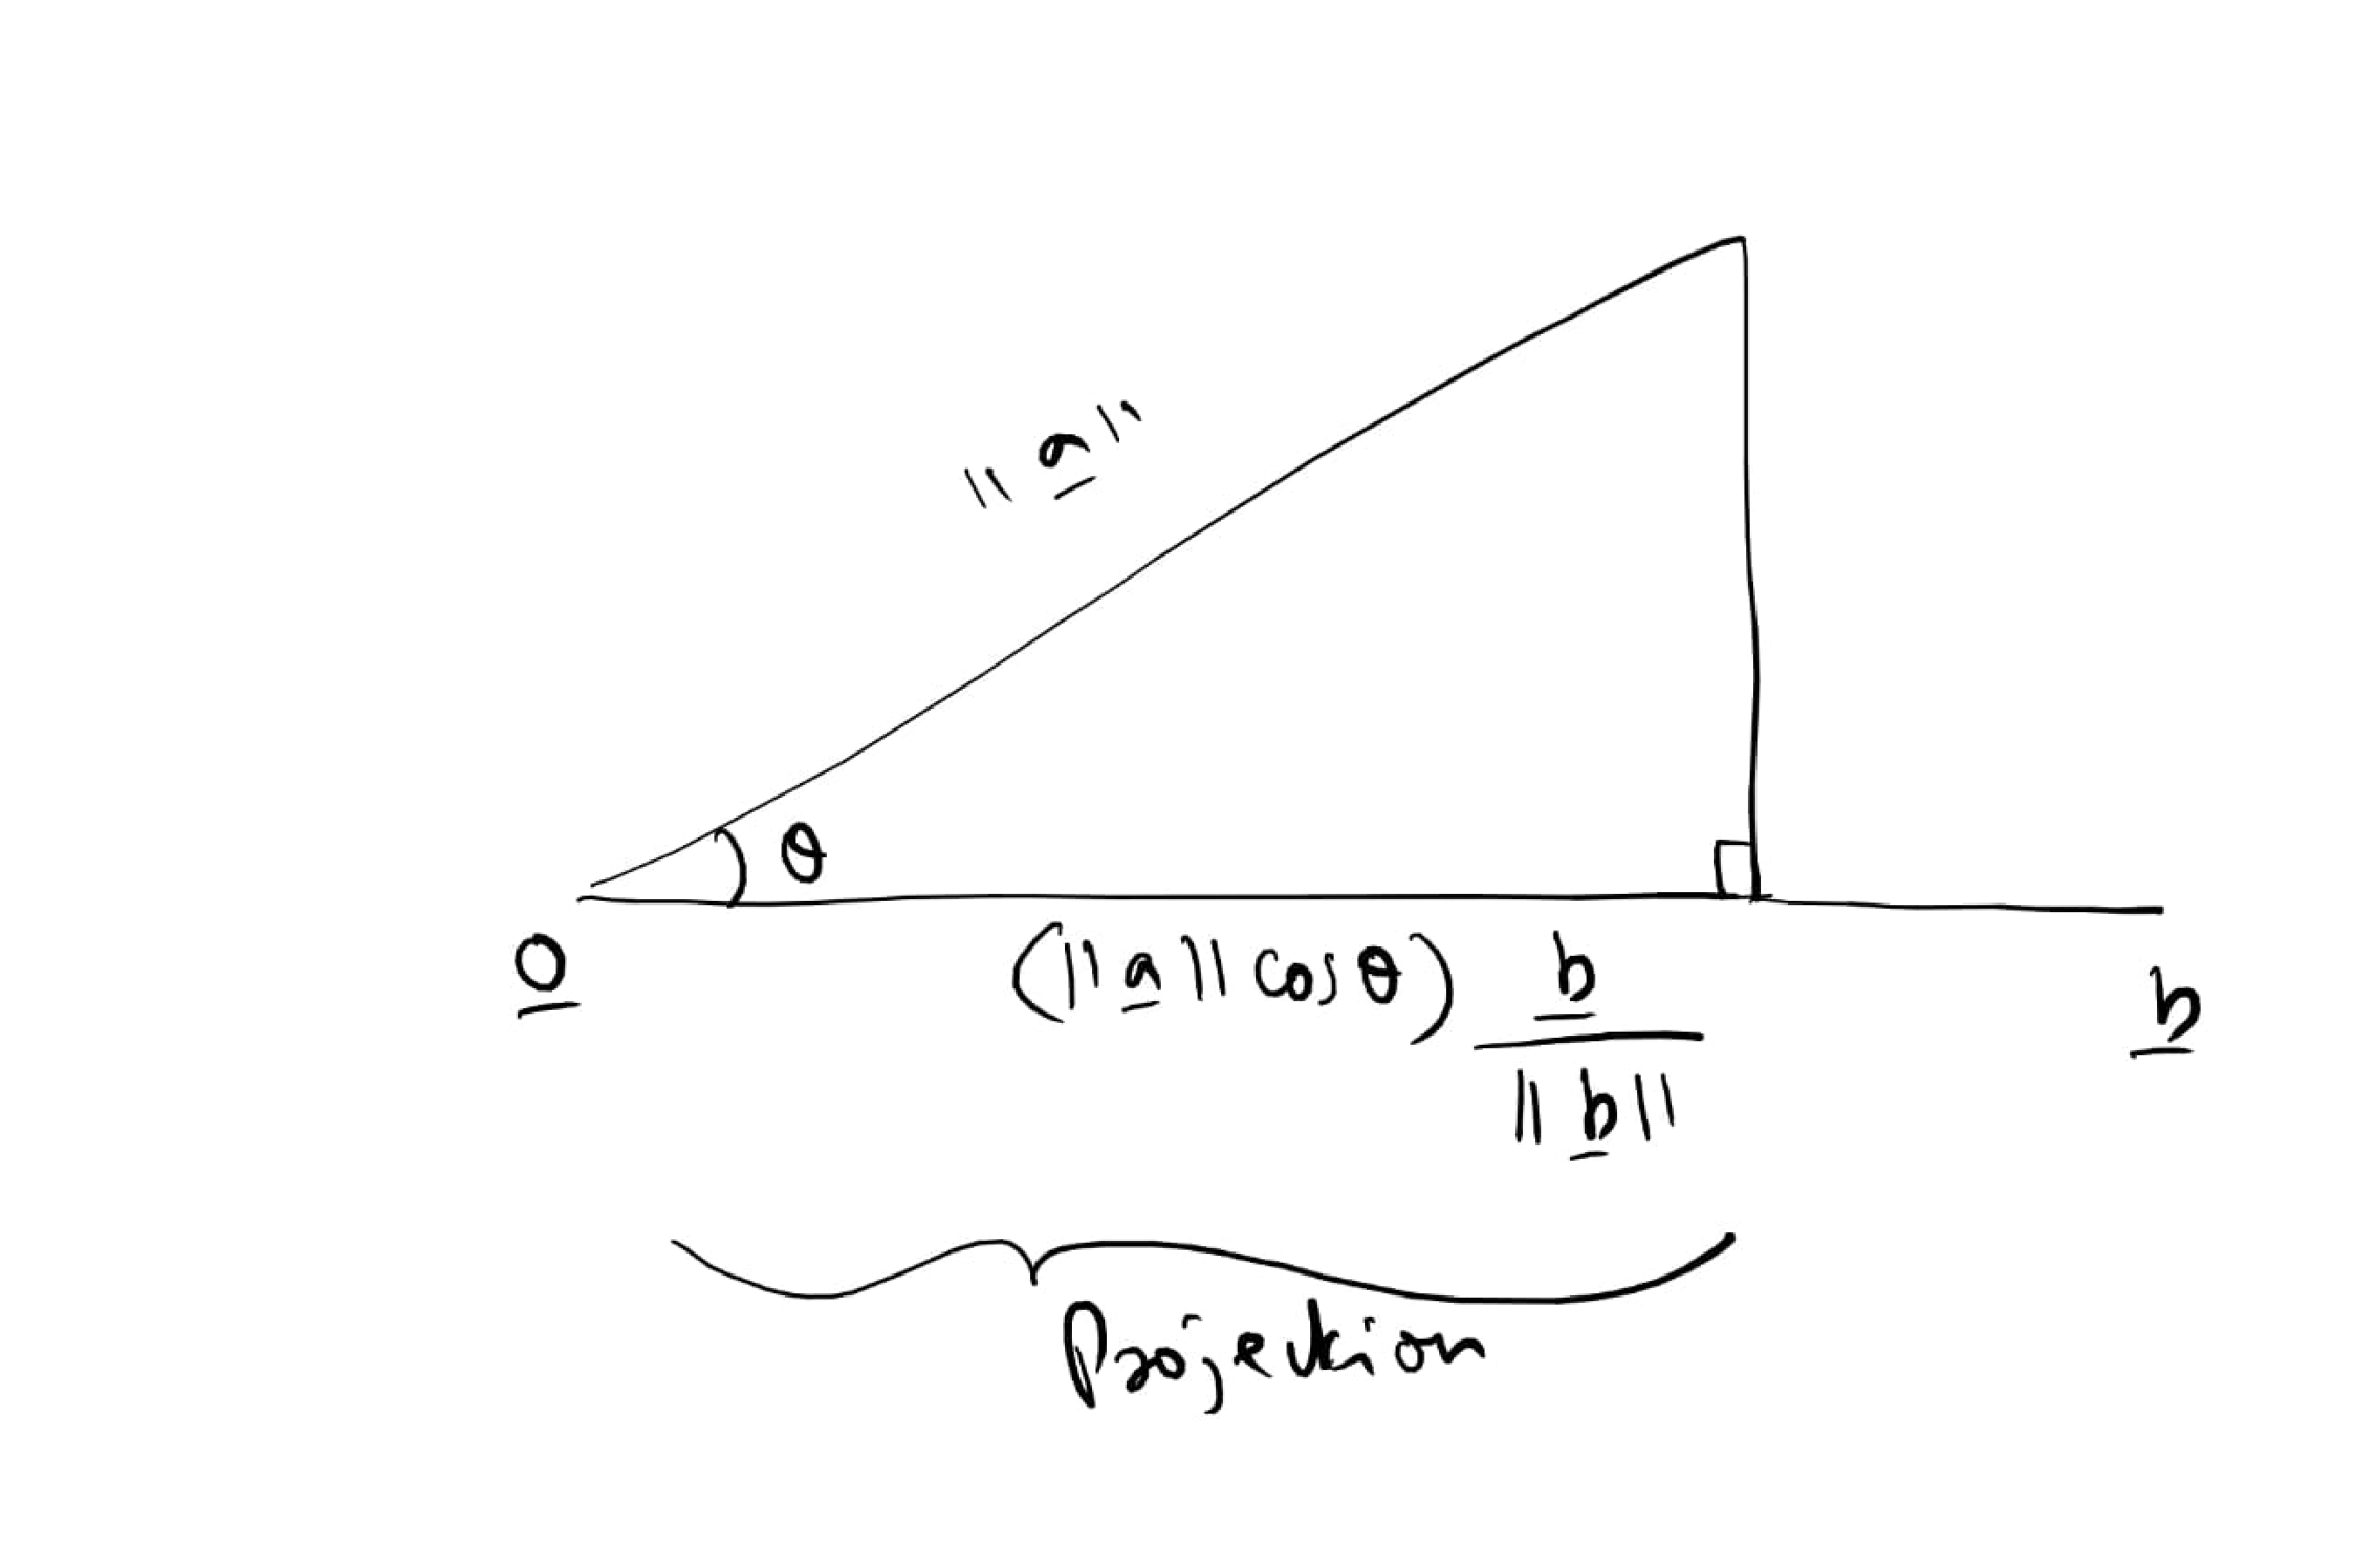
\includegraphics[width=\columnwidth]{./line/figs/line_proj.eps}
\caption{}
\label{fig:line_proj}
\end{figure}
%
Thus, the projection is defined as 
\begin{align}
\brak{\norm{\vec{a}}\cos\theta} \frac{\vec{b}}{\norm{\vec{b}}}
=  \frac{\brak{\vec{a}^T\vec{b}}\norm{\vec{a}}}{\norm{\vec{b}}}\vec{b}
\end{align}
\item Find $\norm{\vec{a}-\vec{b}}$, if 
\begin{align}
\norm{\vec{a}} = 2, 
\norm{\vec{b}} = 3,
\vec{a}^T\vec{b} = 4.
\end{align}
%
\solution 
Let the balanced version of (\ref{eq:solutions/chem/6ato balance}) be
\begin{align}
    \label{eq:solutions/chem/6abalanced}x_{1}HNO_{3}+ x_{2}Ca(OH)_{2}\to x_{3}Ca(NO_{3})_{2}+ x_{4}H_{2}O
\end{align}

which results in the following equations:
\begin{align}
    (x_{1}+ 2x_{2}-2x_{4}) H= 0\\
    (x_{1}-2x_{3}) N= 0\\
    (3x_{1}+ 2x_{2}-6x_{3}- x_{4}) O=0\\
    (x_{2}-x_{3}) Ca= 0
\end{align}

which can be expressed as
\begin{align}
    x_{1}+ 2x_{2}+ 0.x_{3} -2x_{4} = 0\\
    x_{1}+ 0.x_{2} -2x_{3} +0.x_{4}= 0\\
    3x_{1}+ 2x_{2}-6x_{3}- x_{4} =0\\
    0.x_{1} +x_{2}-x_{3} +0.x_{4}= 0
\end{align}

resulting in the matrix equation
\begin{align}
    \label{eq:solutions/chem/6a matrix}
    \myvec{1 & 2 & 0 & -2\\
           1 & 0 & -2 & 0\\
           3 & 2 & -6 & -1\\
           0 & 1 & -1 & 0}\vec{x}
           =\vec{0}
\end{align}

where,
\begin{align}
   \vec{x}= \myvec{x_{1}\\x_{2}\\x_{3}\\x_{4}}
\end{align}

(\ref{eq:solutions/chem/6a matrix}) can be reduced as follows:
\begin{align}
    \myvec{1 & 2 & 0 & -2\\
           1 & 0 & -2 & 0\\
           3 & 2 & -6 & -1\\
           0 & 1 & -1 & 0}
    \xleftrightarrow[R_{3}\leftarrow \frac{R_3}{3}-R_{1}]{R_{2}\leftarrow R_2- R_1}
    \myvec{1 & 2 & 0 & -2\\
           0 & -2 & -2 & 2\\
           0 & -\frac{4}{3} & -2 & \frac{5}{3}\\
           0 & 1 & -1 & 0}\\
    \xleftrightarrow{R_2 \leftarrow -\frac{R_2}{2}}
    \myvec{1 & 2 & 0 & -2\\
          0 & 1 & 1 & -1\\
          0 & -\frac{4}{3} & -2 & \frac{5}{3}\\
          0 & 1 & -1 & 0}\\
    \xleftrightarrow[R_4 \leftarrow R_4- R_2]{R_3 \leftarrow R_3 + \frac{4}{3}R_2}
    \myvec{1 & 2 & 0 & -2\\
           0 & 1 & 1 & -1\\
           0 & 0 & -\frac{2}{3} & \frac{1}{3}\\
           0 & 0 & -2 & 1}\\
    \xleftrightarrow[R_3 \leftarrow -\frac{3}{2}R_3]{R_1 \leftarrow R_1- 2R_2}
    \myvec{1 & 0 & -2 & 0\\
           0 & 1 & 1 & -1\\
           0 & 0 & 1 & -\frac{1}{2}\\
           0 & 0 & -2 & 1}\\
    \xleftrightarrow{R_4\leftarrow R_4 + 2R_3}
    \myvec{1 & 0 & -2 & 0\\
           0 & 1 & 1 & -1\\
           0 & 0 & 1 & -\frac{1}{2}\\
           0 & 0 & 0 & 0}\\
    \xleftrightarrow[R_2\leftarrow R_2-R_3]{R_1\leftarrow R_1 + 2R_3}
    \myvec{1 & 0 & 0 & -1\\
           0 & 1 & 0 & -\frac{1}{2}\\
           0 & 0 & 1 & -\frac{1}{2}\\
           0 & 0 & 0 & 0}
\end{align}

Thus,
\begin{align}
    x_1=x_4, x_2= \frac{1}{2}x_4, x_3=\frac{1}{2}x_4\\
    \implies \quad\vec{x}= x_4\myvec{1\\ \frac{1}{2}\\ \frac{1}{2}\\1} =\myvec{2\\1\\1\\2}
\end{align} 
by substituting $x_4= 2$.

\hfill\break
%\vspace{5mm} 
Hence, (\ref{eq:solutions/chem/6abalanced}) finally becomes
\begin{align}
    2HNO_{3}+ Ca(OH)_{2}\to Ca(NO_{3})_{2}+ 2H_{2}O
\end{align}

%
%\begin{align}
%\norm{\vec{a}-\vec{b}}^2 = \norm{\vec{a}}^2+\norm{\vec{b}}^2
%-2\vec{a}^T\vec{b}
%\end{align}
%
\item If $\vec{a}$ is a unit vector and 
%
\begin{align}
\brak{\vec{x}-\vec{a}}\brak{\vec{x}+\vec{a}} = 8, 
\end{align}
%
then find $\vec{x}$.
%
\\
\solution 
%
\begin{align}
\brak{\vec{x}-\vec{a}}\brak{\vec{x}+\vec{a}} &= \norm{\vec{x}}^2-\norm{\vec{a}}^2
\\
\implies \norm{\vec{x}}^2 &= 9 \text{ or, } \norm{\vec{x}} = 3.
\end{align}
%
\item Given
\begin{align}
\vec{a}=\myvec{2\\1\\3},
\vec{b}=\myvec{3\\5\\-2},
\end{align}
find $\norm{\vec{a} \times \vec{b}}$.
%
\\
\solution Use \eqref{eq:tri_cross_prod}.
%
\item Find a unit vector perpendicular to each of the vectors
$\vec{a}+\vec{b}$ and $\vec{a}-\vec{b}$, where 
\begin{align}
\vec{a}=\myvec{1\\1\\1},
\vec{b}=\myvec{1\\2\\3}.
\end{align}
%
\solution If $\vec{x}$ is the desired vector, 
%
\begin{align}
\brak{\vec{a}+\vec{b}}^T\vec{x}=0
\\
\brak{\vec{a}-\vec{b}}^T\vec{x}=0
\end{align}
%
resulting in the matrix equation 
%
\begin{align}
\myvec{2 & 3 & 4\\
0 & -1 & -2}\vec{x} = 0
\end{align}
%
Performing row operations, 
%
\begin{align}
\myvec{2 & 3 & 4\\
0 & -1 & -2}
\xleftrightarrow[R_2 \leftarrow -R_2]{R_1\leftarrow R_1+3R_2}
\myvec{
2 & 0 & -2\\
0 & -1 & -2
} 
\\
\xleftrightarrow{R_1\leftarrow \frac{R_1}{2}}
\myvec{
1 & 0 & -1\\
0 & 1 & 2
} 
\implies \myvec{x_1\\x_2\\x_3} = x_3\myvec{1\\-2\\1}
\end{align}
%
The desired unit vector is then obtained as
%
\begin{align}
\vec{x} =\frac{\myvec{1\\-2\\1}}{\norm{\myvec{1\\-2\\1}}}
=\frac{1}{\sqrt{6}}\myvec{1\\-2\\1}
\end{align}
\item Show that 
$\vec{A}=\myvec{-2\\3\\5}, \vec{B}=\myvec{1\\2\\3}, \vec{C}=\myvec{7\\0\\-1}$, are collinear.
%
\\
\solution See Problem \ref{prob:line_coll_3d}.
\item If 
$\vec{A}=\myvec{1\\1\\1}, \vec{B}=\myvec{2\\5\\0}, \vec{C}=\myvec{3\\2\\-3}$  and $ \vec{D}=\myvec{1\\-6\\-1}$,
show that  $\vec{A}-\vec{B}$ and $\vec{C}-\vec{D}$ are collinear.
%
\\
\solution 
%
\begin{align}
\vec{A}-\vec{B} &= \myvec{-1\\-4\\1}
\\
\vec{C}-\vec{D} &= \myvec{2\\8\\-2}
\end{align}
%
%
\begin{align}
\because -2\brak{\vec{A}-\vec{B}} =  \vec{C}-\vec{D},
\end{align}
%
$\vec{A}-\vec{B}$ and $\vec{C}-\vec{D}$ are collinear.

\item Let $\norm{\vec{a}} = 3, \norm{\vec{b}}= 4, \norm{\vec{c}} = 5$ such that each vector is perpendicular to the other two.  Find $\norm{\vec{a}+\vec{b}+\vec{c}}$.
%
\\
\solution Given that 
%
\begin{align}
\label{eq:line_pair_orth}
 \vec{a}^T \vec{b} =  \vec{b}^T\vec{c}= \vec{c}^T\vec{a} = 0.
\end{align}
%
Then, 
%
\begin{multline}
\norm{\vec{a}+\vec{b}+\vec{c}}^2 = \norm{\vec{a}}^2+\norm{\vec{b}}^2+\norm{\vec{c}}^2
\\
+ \vec{a}^T \vec{b} +  \vec{b}^T\vec{c}+ \vec{c}^T\vec{a}.
\end{multline}
%
which reduces to 
%
\begin{align}
\norm{\vec{a}+\vec{b}+\vec{c}}^2 = \norm{\vec{a}}^2+\norm{\vec{b}}^2+\norm{\vec{c}}^2
\end{align}
%
using \eqref{eq:line_pair_orth}
%
\item Given 
\begin{align}
\label{eq:line_vec_sum_0}
 \vec{a}+\vec{b}+\vec{c} = \vec{0}, 
\end{align}
evaluate 
\begin{align}
 \vec{a}^T\vec{b}+\vec{b}^T\vec{c}+\vec{c}^T\vec{a},
\end{align}
given that $\norm{ \vec{a}}=3, \norm{ \vec{b}}= 4$ and $\norm{ \vec{c}} = 2 $.
%
\\
\solution Multiplying \eqref{eq:line_vec_sum_0} with $\vec{a}, \vec{b}, \vec{c}$,
\begin{align}
%\label{eq:line_vec_sum_0}
\norm{ \vec{a}}^2+\vec{a}^T\vec{b}+\vec{a}^T\vec{c} &= 0
\\
\vec{a}^T\vec{b}+\norm{ \vec{b}}^2+\vec{b}^T\vec{c} &= 0
\\
+\vec{c}^T\vec{a}+\vec{b}^T\vec{c}+\norm{ \vec{c}}^2 &= 0
\end{align}
%
Adding all the above equations and rearranging,
\begin{multline}
%\label{eq:line_vec_sum_0}
 \vec{a}^T\vec{b}+\vec{b}^T\vec{c}+\vec{c}^T\vec{a} = -\frac{\norm{ \vec{a}}^2+\norm{ \vec{b}}^2+\norm{ \vec{c}}^2}{2}
\end{multline}
%
\item Let $\bm{\alpha} = \myvec{3\\-1\\0}, \bm{\beta} = \myvec{2\\1\\-3}$.  Find $\bm{\beta}_1, \bm{\beta}_2 $ such that $\bm{\beta}=\bm{\beta}_1+\bm{\beta}_2, \bm{\beta}_1 \parallel  \bm{\alpha} $ and $\bm{\beta}_2 \perp \bm{\alpha} $.
%
\label{prob:line_gram_schmidt}
\\
\solution Let $\beta_1 = k\alpha$.  Then, 
%
\begin{align}
\bm{\beta} &= k\bm{\alpha}+\bm{\beta}_2
\\
\implies k &= \frac{\bm{\alpha}^T\bm{\beta}}{\norm{\bm{\alpha}}^2}
\end{align}
%
and 
%
\begin{align}
\bm{\beta}_2 &= \bm{\beta}-k\bm{\alpha}
\end{align}
%
This process is known as {\em Gram-Schmidth orthogonalization}.
\item Find a unit vector that makes an angle of $90\degree, 60\degree$ and $30\degree$ with the positive x, y and z axis respectively.
%
\\
\solution
The direction vector is
%
\begin{align}
\label{eq:line_dir_cos}
\vec{x} &= \myvec{\cos 90\degree\\\cos 60\degree \\ \cos 30\degree} = \myvec{0 \\ \frac{1}{2}\\\frac{\sqrt{3}}{2}}
\end{align}
%
$\because \norm{\vec{x}}=1$, it is the desired unit vector.
%
\item Find the 
distance between the lines 
\begin{align}
L_1: \quad \vec{x} &= \myvec{1\\2\\-4} + \lambda_1\myvec{2 \\ 3 \\6}
\\
L_2: \quad \vec{x} &= \myvec{3\\3\\-5} + \lambda_2\myvec{2 \\ 3 \\6}
\end{align}
\label{prob:line_dist_parallel}
%
\solution Both the lines have the same direction vector, so the lines are parallel. 
The following code plots 
%
\begin{lstlisting}
codes/line/line_dist_parallel.py
\end{lstlisting}
Fig. \ref{fig:line_dist_parallel_py} 
%
\begin{figure}[!ht]
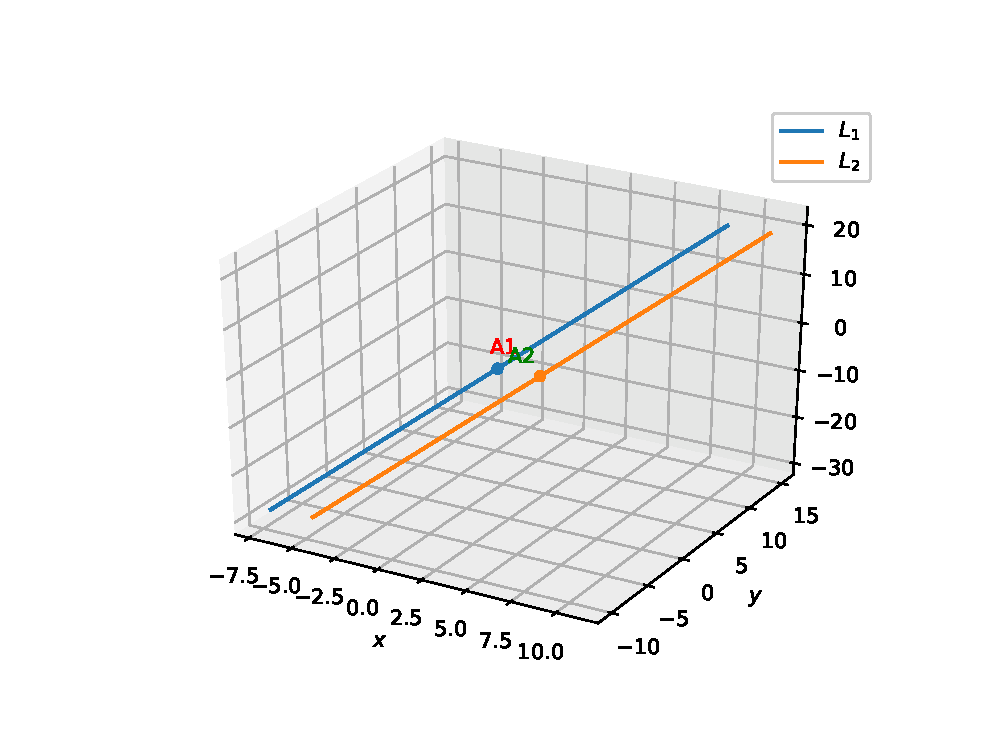
\includegraphics[width=\columnwidth]{./line/figs/line_dist_parallel_py.eps}
\caption{}
\label{fig:line_dist_parallel_py}
\end{figure}
%
%
From Fig. \ref{fig:line_dist_parallel}, the distance is
%
\begin{figure}
\centering
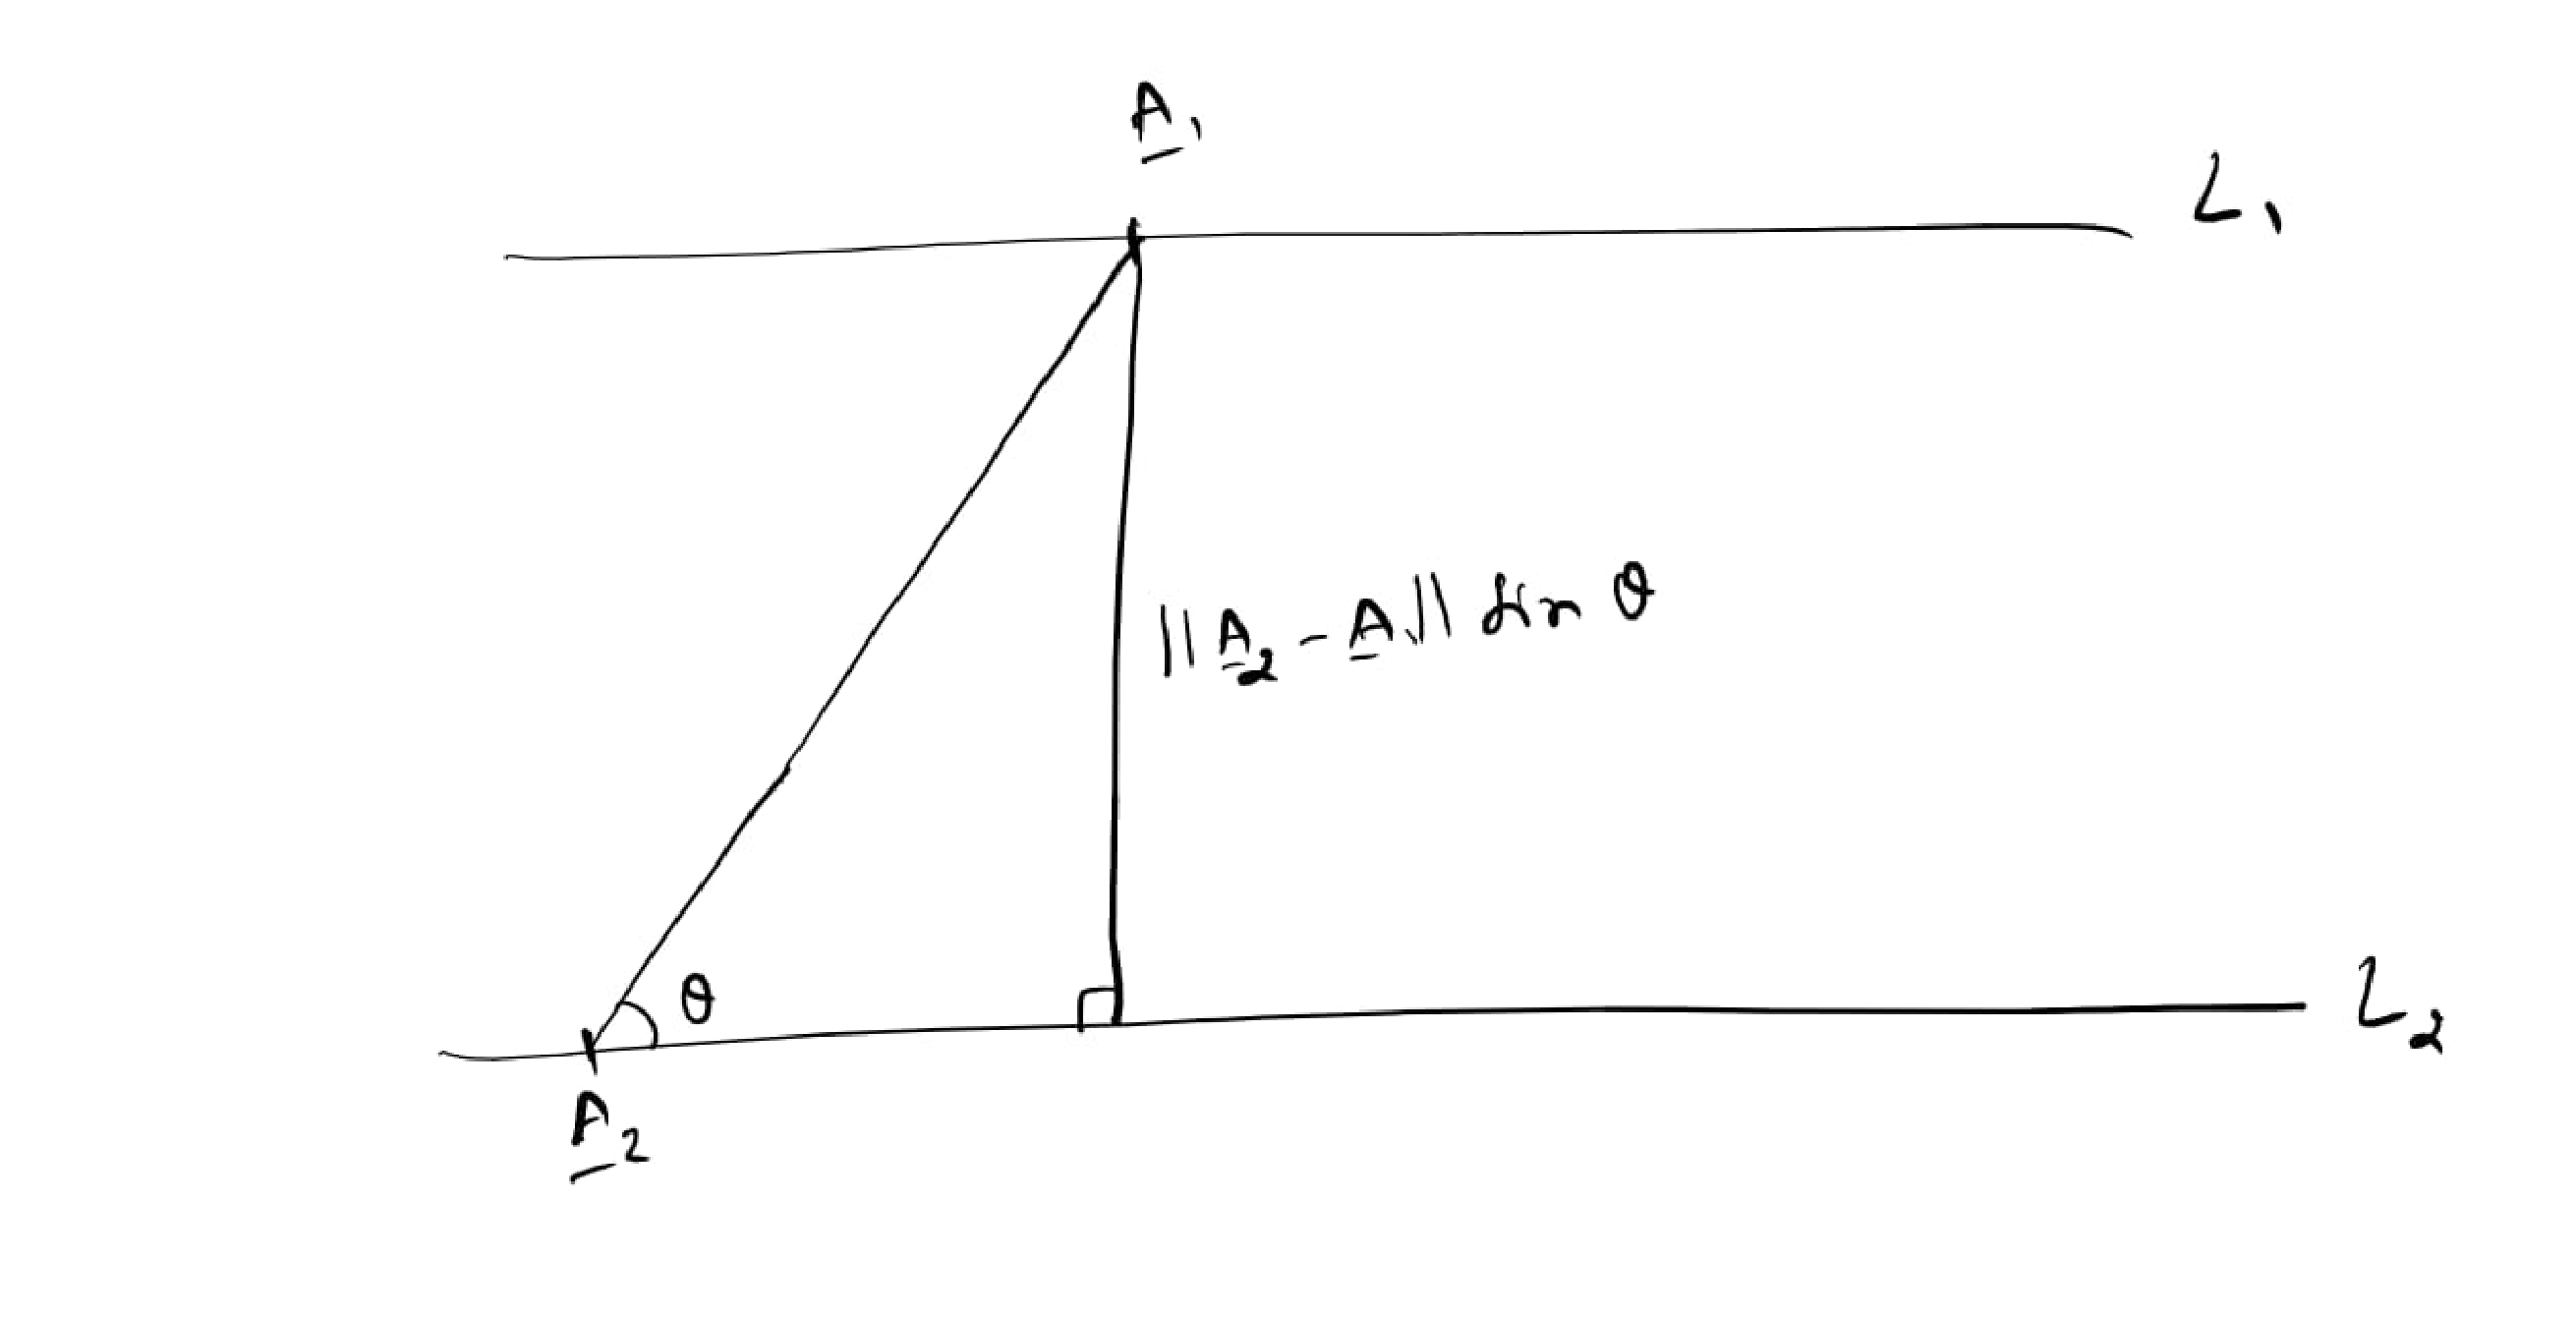
\includegraphics[width=\columnwidth]{./line/figs/line_dist_parallel.eps}
\caption{}
\label{fig:line_dist_parallel}
\end{figure}
%
\begin{align}
\label{eq:line_dist_parallel}
\vec{\norm{\vec{A}_2-
\vec{A}_1}}\sin\theta =\frac{\norm{\vec{m}\times \brak{\vec{A}_2-
\vec{A}_1}}}{\norm{\vec{m}}}
\end{align}
%
where 
%
\begin{align}
\vec{A}_1 = \myvec{1\\2\\-4},
\vec{A}_2 = \myvec{3\\3\\-5},
\vec{m}=\myvec{2 \\ 3 \\6}
\end{align}
%

\item Find the shortest distance between the lines 
\begin{align}
L_1: \quad \vec{x} &= \myvec{1\\1\\0} + \lambda_1\myvec{2 \\ -1 \\1}
\\
L_2: \quad \vec{x} &= \myvec{2\\1\\-1} + \lambda_2\myvec{3 \\ -5 \\2}
\end{align}
\label{prob:line_dist_skew}
%
\solution  In the given  problem
\begin{align}
\vec{A}_1= \myvec{1\\1\\0}, \vec{m}_1=\myvec{2 \\ -1 \\1},
\vec{A}_2= \myvec{2\\1\\-1}, \vec{m}_2 =\myvec{3 \\ -5 \\2}.
\end{align}
%
The lines will intersect if
%
\begin{align}
\myvec{1\\1\\0} + \lambda_1\myvec{2 \\ -1 \\1}
= \myvec{2\\1\\-1} + \lambda_2\myvec{3 \\ -5 \\2}
\\
\implies \lambda_1\myvec{2 \\ -1 \\1} - \lambda_2\myvec{3 \\ -5 \\2} &= \myvec{2\\1\\-1}-\myvec{1\\1\\0}  
\\
\implies \myvec{2 & 3 \\ -1 & -5 \\ 1 & 2}\myvec{\lambda_1\\ \lambda_2} = \myvec{1\\0\\-1}
\end{align}
%
Row reducing the augmented matrix,
%
\begin{align}
\myvec{
2 & 3 & 1 
\\
-1 & -5 & 0
\\
1 & 2 & -1
}
\xleftrightarrow[]{R_3\leftrightarrow R_1}
\myvec{
1 & 2 & -1
\\
-1 & -5 & 0
\\
2 & 3 & 1 
}
\\
\xleftrightarrow[]{\substack{R_2= R_1+R_2\\R_3 = 2R_1-R_3}}
\myvec{
1 & 2 & -1
\\
0 & -3 & -1
\\
0 & 1 & -3 
}
\xleftrightarrow[]{R_2\leftrightarrow R_3}
\myvec{
1 & 2 & -1
\\
0 & 1 & -3 
\\
0 & -3 & -1
}
\\
\xleftrightarrow[]{R_3=3R_2+R_3}
\myvec{
1 & 2 & -1
\\
0 & 1 & -3 
\\
0 & 0 & -10
}
\end{align}
%
The above matrix has $rank = 3$.  Hence, the lines do not intersect.  Note that the lines are not parallel but they  lie on parallel planes.  Such lines are known as {\em skew} lines.  
The following code plots 
Fig. \ref{fig:line_dist_skew} 
%
\begin{lstlisting}
codes/line/line_dist_skew.py
\end{lstlisting}
%
\begin{figure}[!ht]
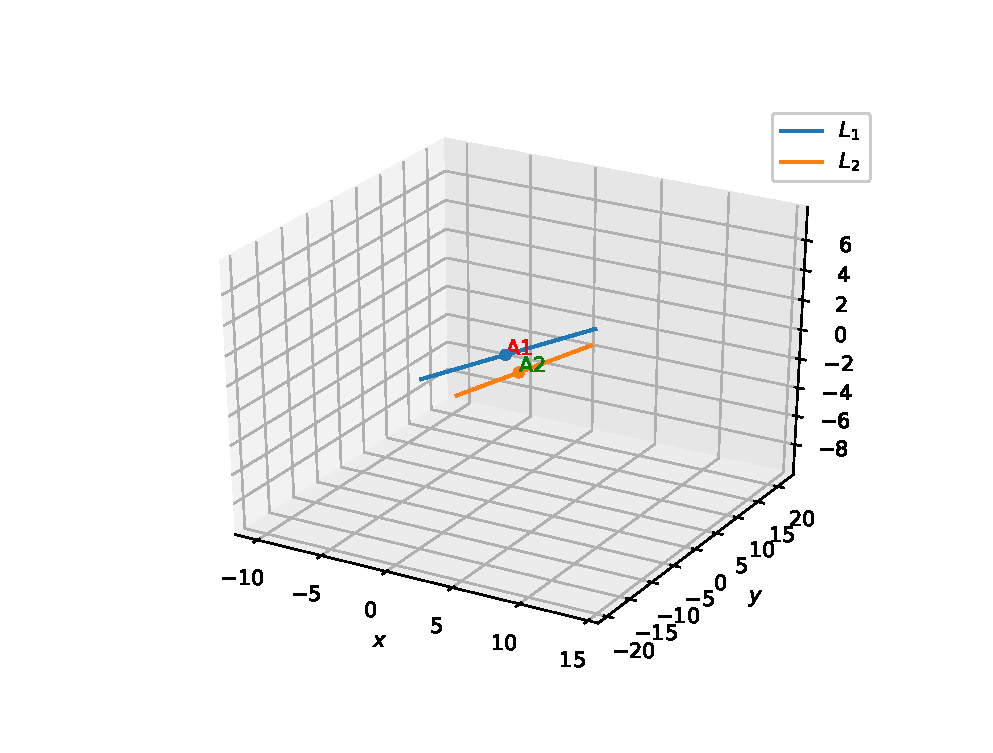
\includegraphics[width=\columnwidth]{./line/figs/line_dist_skew.eps}
\caption{}
\label{fig:line_dist_skew}
\end{figure}
%

The normal to both the lines (and corresponding planes) is 
%
\begin{align}
\label{eq:line_dist_skew_normal}
\vec{n} = \vec{m}_1\times\vec{m}_2
\end{align}
%
The equation of the second plane is then obtained as
%
\begin{align}
\label{eq:line_dist_skew_plane2}
\vec{n}^T \vec{x} = \vec{n}^T \vec{A}_2 
\end{align}
%
The distance from $\vec{A}_1$ to the above line is then obtained using 
\eqref{eq:line_pt_dist} as
%
\begin{align}
\label{eq:line_dist_skew}
\frac{\abs{\vec{n}^T\brak{\vec{A}_2-\vec{A}_1}}}{\norm{\vec{n}}}
=
\frac{\abs{\brak{\vec{A}_2-\vec{A}_1}^T\brak{\vec{m}_1\times\vec{m}_2}}}{\norm{\vec{m}_1\times\vec{m}_2}}
\end{align}
%

\item Find the distance of the plane 
\begin{align}
\myvec{2 & -3 & 4}\vec{x}-6  = 0
\end{align}
%
from the origin.
\\
\solution From \eqref{eq:line_pt_dist}, the distance is obtained as
%
\begin{align}
\frac{\abs{c}}{\norm{\vec{n}}} &= \frac{6}{\sqrt{2^2+3^2+4^2}}
\\
&= \frac{6}{\sqrt{29}}
\end{align}
%

\item Find the equation of a plane which is at a distance of $\frac{6}{\sqrt{29}}$ from the origin and has  normal vector $\vec{n}=\myvec{2\\-3\\4}$.
%
\\
\solution From the previous problem, the desired equation is
%
\begin{align}
\myvec{2 & -3 & 4}\vec{x}-6  = 0
\end{align}
%

\item Find the unit normal vector of the plane 
\begin{align}
\myvec{6 & -3 & -2}\vec{x}  = 1.
\end{align}
%
\solution The normal vector is 
%
\begin{align}
\vec{n} = \myvec{6 & -3 & -2}
\\
\because \norm{\vec{n}} = 7,
\end{align}
%
the unit normal vector is 
%
\begin{align}
\frac{\vec{n}}{\norm{\vec{n}}} = \frac{1}{7}\myvec{6 & -3 & -2}
\end{align}
%
\item Find the coordinates of the foot of the perpendicular drawn from the origin to the plane 
\begin{align}
\label{eq:line_foot_perp}
\myvec{2 & -3 & 4}\vec{x}-6  = 0
\end{align}
%
\solution The normal vector is 
%
\begin{align}
\vec{n}=\myvec{2 \\ -3 \\ 4}
\end{align}
%
Hence, the foot of the perpendicular from the origin is $\lambda \vec{n}$.  Substituting in \eqref{eq:line_foot_perp},
\begin{align}
\lambda \norm{\vec{n}}^2 = 6  \implies \lambda = \frac{6}{\norm{\vec{n}}^2} = \frac{6}{29}
\end{align}
%
Thus, the foot of the perpendicular is
%
\begin{align}
\frac{6}{29}\myvec{2 \\ -3 \\ 4}
\end{align}
%
\item Find the equation of the plane which passes through the point $\vec{A}=\myvec{5\\2\\-4}$ and perpendicular to the line with direction vector $\vec{n}=\myvec{2\\3\\-1}$.
%
\\
\solution  The normal vector to the plane is $\vec{n}$. Hence from \eqref{eq:line_norm_vec}, the equation of the plane is 
%
\begin{align}
\vec{n}^T\brak{\vec{x}-\vec{A}} &= 0
\\
\implies \myvec{2\\3\\-1}\vec{x} &=\myvec{2&3&-1}\myvec{5\\2\\-4}
\\
&=20
\end{align}
%
%The following 
%%
%\begin{lstlisting}
%codes/line/plane_3d.py
%\end{lstlisting}
%%
%\begin{figure}[!ht]
%\includegraphics[width=\columnwidth]{./line/figs/plane_3d.eps}
%\caption{}
%\label{fig:plane_3d}
%\end{figure}
%

\item Find the equation of the plane passing through 
$
\bm{R} = \myvec{2\\5\\-3},
\bm{S}= \myvec{-2\\-3\\5}
$ 
and 
$
\bm{T}= \myvec{5\\3\\-3}.
$
\label{prob:plane_3pts}
\\
\solution  If the equation of the plane be 
\begin{align}
\vec{n}^T\vec{x} &= c,
\\
\vec{n}^T\vec{R}=\vec{n}^T\vec{S}=\vec{n}^T\vec{T}&= c,
\\
\implies \myvec{\vec{R}-\vec{S} & \vec{S}-\vec{T}}^T\vec{n} &= 0
\end{align}
%
after some algebra.
Using row reduction on the above matrix, 
\begin{align}
\myvec{4 & 8 &-8 \\ -7  & -6 & 8} \xleftrightarrow[]{R_1\leftarrow \frac{R_1}{4}}\myvec{1 & 2 &-2 \\ -7  & -6 & 8}
\\
\xleftrightarrow[]{R_2\leftarrow R_2 + 7R_1}
\myvec{
1 & 2 &-2 
\\ 
0  & 8 & -6
}
\xleftrightarrow[]{R_2\leftarrow \frac{R_2}{2}}
\myvec{
1 & 2 &-2 
\\ 
0  & 4 & -3
}
\\
\xleftrightarrow[]{R_1\leftarrow 2R_1-R_2}
\myvec{
2 & 0 &-1 
\\ 
0  & 4 & -3
}
\end{align}
%
Thus, 
\begin{align}
\vec{n} &= \myvec{\frac{1}{2}\\\frac{3}{4}\\1} = \myvec{2\\3\\4} \text{ and}
\\
c = \vec{n}^{T}\vec{T} = 7
\end{align}
%
Thus, the equation of the plane is 
%
\begin{align}
\myvec{2 & 3 & 4}\vec{n} = 7
\end{align}
%
Alternatively, the normal vector to the plane can be obtained as
%
\begin{align}
\vec{n} = \brak{\vec{R}-\vec{S}} \times \brak{\vec{S}-\vec{T}}
\end{align}
%
The equation of the plane is then obtained from \eqref{eq:line_norm_vec} as 
%
\begin{align}
\label{eq:plane_3pts_cross}
\vec{n}^T\brak{\vec{x}-\vec{T}} = \sbrak{\brak{\vec{R}-\vec{S}} \times \brak{\vec{S}-\vec{T}}}^T\brak{\vec{x}-\vec{T}} = 0
\end{align}
%

\item Find the equation of the plane with intercepts 2, 3 and 4 on the x, y and z axis respectively.
\\
\solution From the given information, the plane passes through the points \myvec{2\\0\\0}, \myvec{0\\3\\0} and \myvec{0\\0\\4} respectively. The equation can be obtained using Problem \ref{prob:plane_3pts}.

\item Find the equation of the plane passing through the intersection of the planes 
%
\begin{align}
\label{eq:plane_2p_1pt_1}
\myvec{1 & 1 & 1}\vec{x}&=6  
\\
\myvec{2 & 3 & 4}\vec{x}&=-5
\label{eq:plane_2p_1pt_2}
\end{align}
%
and the point \myvec{1\\1\\1}.
\\
\solution The intersection of the planes is obtained by row reducing the augmented matrix as
%
\begin{align}
\myvec{
1 & 1 & 1 & 6
\\
2 & 3 & 4 & -5
}
\xleftrightarrow[]{R_2 = R_2 -2R_1}
\myvec{
1 & 1 & 1 & 6
\\
0 & 1 & 2 & -17
}
\\
\xleftrightarrow[]{R_1 = R_1 -R_2}
\myvec{
1 & 0 & -1 & 23
\\
0 & 1 & 2 & -17
}
\\
\implies 
\vec{x} = \myvec{23\\-17\\0}+\lambda\myvec{1\\-2\\1}
\end{align}
%
Thus, \myvec{23\\-17\\0} is another point on the plane.  The normal vector to the plane is then obtained as
The normal vector to the plane is then obtained as
%
\begin{align}
\brak{ \myvec{1\\1\\1}-\myvec{23\\-17\\0}}\times \myvec{1\\-2\\1} 
\end{align}
%
which can be obtained by row reducing the matrix
\begin{align}
\myvec{
1 & -2 & 1
\\
-22 & 18 & 1
}
\xleftrightarrow[]{R_2 = R_2+22R_1}
\myvec{
1 & -2 & 1
\\
0  & -26 & 23
}
\\
\xleftrightarrow[]{R_1 = 13R_1-R_2}
\myvec{
13 & 0 & -10
\\
0  & -26 & 23
}
\\
\implies \vec{n} = \myvec{\frac{10}{13}\\\frac{23}{26}\\1} = \myvec{20\\23\\26}
\end{align}
%
Since the plane passes through \myvec{1\\1\\1}, using 
 \eqref{eq:line_norm_vec},
%
\begin{align}
\myvec{20 & 23 & 26}\brak{\vec{x}- \myvec{1\\1\\1}} &= 0
\\
\implies 
\myvec{20 & 23 & 26}\vec{x} &= 69
\end{align}
%
Alternatively, the plane passing through the intersection of \eqref{eq:plane_2p_1pt_1} and 
\eqref{eq:plane_2p_1pt_2} has the form 
%
\begin{align}
\label{eq:plane_2p_1pt_lam}
\myvec{1 & 1 & 1}\vec{x} + \lambda \myvec{2 & 3 & 4}\vec{x} &=6 -5\lambda  
\end{align}
%
Substituting \myvec{1\\1\\1} in the above, 
%
\begin{align}
\myvec{1 & 1 & 1}\myvec{1\\1\\1} + \lambda \myvec{2 & 3 & 4}\myvec{1\\1\\1} &=6 -5\lambda  
\\
\implies 3 + 9\lambda &= 6-5\lambda
\\
\implies &\lambda = \frac{3}{14}
\end{align}
%
Substituting this value of $\lambda $ in \eqref{eq:plane_2p_1pt_lam} yields the equation of the plane.

\item Show that the lines 
\label{prob:line_coplanar}
%
\begin{align}
\frac{x+3}{-3} = \frac{y-1}{1} &= \frac{z-5}{5}, 
\\
\frac{x+1}{-1} = \frac{y-2}{2} &= \frac{z-5}{5} 
\end{align}
%
are coplanar.
\\
\solution Since the given lines have different direction vectors, they are not parallel.  From Problem \eqref{prob:line_dist_skew}, the lines are coplanar if the distance between them is 0, i.e. they intersect.  This is possible if 
%
\begin{align}
\label{eq:line_coplanar}
\brak{\vec{A}_2-\vec{A}_1}^T\brak{\vec{m}_1\times\vec{m}_2} = 0
\end{align}
%
From the given information, 
%
\begin{align}
\vec{A}_2-\vec{A}_1 = \myvec{-3\\1\\5}-\myvec{-1\\2\\5} = \myvec{-2\\-1\\0}
\end{align}
%
$\vec{m}_1\times \vec{m}_2$ is obtained by row reducing the matrix
%
\begin{align}
\myvec{
-1 & 2 & 5
\\
-3 & 1 & 5
}
\xleftrightarrow[]{R_2=\frac{R_2-3R_1}{5}}
\myvec{
-1 & 2 & 5
\\
0 & 1 & 2
}
\\
\xleftrightarrow[]{R_1=-R_1+2R_2}
\myvec{
1 & 0 & -1
\\
0 & 1 & 2
}
\implies \myvec{-1 \\ 2 \\ 5}
\times \myvec{-3 \\ 1 \\ 5}
=\myvec{1\\-2\\1}
\end{align}
%
The LHS of \eqref{eq:line_coplanar} is 
\begin{align}
\myvec{-2 & -1 & 0}
\myvec{1\\-2\\1} = 0
\end{align}
%
which completes the proof.  Alternatively, the lines are coplanar if
%
\begin{align}
\mydet{\vec{A}_1-\vec{A}_2 & \vec{m}_1 & \vec{m}_2} = 0
\end{align}
%

\item Find the angle between the two planes
\label{prob:planes_angle}
\begin{align}
\myvec{2 & 1 & -2}\vec{x}&=5
\\
\myvec{3 &-6 & -2}\vec{x}&=7.
\end{align}
%
\solution The angle between two planes is the same as the angle between their normal vectors.  This can be obtained from \eqref{eq:line_scalar_prod}.

\item Find the angle between the two planes
\begin{align}
\myvec{2 & 2 & -2}\vec{x}&=5
\\
\myvec{3 &-6 & 2}\vec{x}&=7.
\end{align}
%
\solution See Problem \eqref{prob:planes_angle}.
%
\item Find the distance of a point \myvec{2\\5\\-3} from the plane
\begin{align}
\myvec{6 & -3 & 2}\vec{x}=4
\end{align}
%
\\
\solution Use \eqref{eq:line_pt_dist}.
\item Find the angle between the line 
%
\begin{align}
L: \quad \frac{x+1}{2} = \frac{y}{3} = \frac{z-3}{6} 
\end{align}
%
and
%
the plane 
\begin{align}
P: \quad \myvec{10 & 2 & -11}\vec{x}=3
\end{align}
%
\label{prob:plane_angle_line}
%
\solution The angle between the direction vector of $L$ and normal vector of $P$ is 
%
\begin{align}
\cos \theta &= \frac{\abs{\myvec{10 & 2 & -11}\myvec{2\\3\\6}}}{\sqrt{225}\times \sqrt{49}} = \frac{8}{21}
\end{align}
%
Thus, the desired angle is $90\degree -\theta$.
\item Find the equation of the plane that contains the point $\myvec{1\\-1\\2}$ and is perpedicular to each of the planes
\begin{align}
\myvec{2 & 3 & -2}\vec{x}&=5
\\
\myvec{1 & 2 & -3}\vec{x}&=8
\end{align}
%
\solution The normal vector to the desired plane is $\perp$ the normal vectors of both the given planes.  Thus,
%
\begin{align}
\vec{n} = \myvec{2 \\ 3 \\ -2} \times \myvec{1 \\ 2 \\ -3}
\end{align}
%
The equation of the plane is then obtained as
%
\begin{align}
\vec{n}^T\brak{\vec{x}-\vec{A}} = 0
\end{align}
%
\item Find the distance between the point $\vec{P}=\myvec{6\\5\\9}$ and the plane determined by the points $\bm{A}=\myvec{3\\-1\\2}, \bm{B}=\myvec{5\\2\\4}$ and $\bm{C}=\myvec{-1\\-1\\6}$.
%
\\
\solution Find the equation of the plane using Problem \ref{prob:plane_3pts}.  Find the distance using \eqref{eq:line_pt_dist}.
%
\item Find the coordinates of the point where the line through the points
$
\vec{A}=\myvec{3\\4\\1}, 
\vec{B}=\myvec{5\\1\\6}
$
crosses the XY plane.
%
\\
\solution The equation of the line is 
%
\begin{align}
\vec{x} &= \vec{A}+\lambda\brak{\vec{B}-\vec{A}}
\\
&= \myvec{3\\4\\1} + \lambda \myvec{2\\-3\\5}
\end{align}
%
The line  crosses the XY plane for $x_3 = 0 \implies \lambda = -\frac{1}{5}$. Thus, the desired point is
%
\begin{align}
 \myvec{3\\4\\1} -\frac{1}{5}\myvec{2\\-3\\5} = \frac{1}{5}\myvec{13\\23\\0}
\end{align}
%
\item Show that the function given by $f(x) = 7x – 3$ is increasing on $\vec{R}$.
\\
\solution A function is said to be increasing if
\begin{align}
x_2> x_1 &\implies f(x_2)> f(x_1)
\\
\implies \frac{f(x_2)-f(x_1)}{x_2 - x_1}  &> 0
\label{eq:line_inc_12}
\end{align}
%
Letting $x_1 = x, x_2 = x+h$ in \eqref{eq:line_inc_12}, this results in 
\begin{align}
\frac{f(x+h)-f(x)}{h} > 0
\label{eq:line_slope}
\end{align}
In the given problem, 
\begin{align}
\frac{f(x+h)-f(x)}{h} = 7 > 0
\end{align}
%
Hence, the given function is increasing.
%
%
\item A funcion $f(x)$ is increasing if 
\label{them:inc_der_def}
\begin{align}
f^{\prime}(x)=\lim_{h\to 0} \frac{f(x+h)-f(x)}{h} & > 0
\end{align}
%
$f^{\prime}(x)$ is defined as the {\em derivative} of $f(x)$.
The function is decreasing if $f^{\prime}(x) < 0$.  
%
\item The funcion $f(x) = ax+b, a \ne 0$ is increasing if $f^{\prime}(x) = a > 0$.  Else, it is decreasing.
\label{them:line_inc}
%

\item Find the maximum and minimum values, if any, of the function given by 
%
\begin{align}
\label{eq:line_der_def_prob}
f(x) = x, x \in \brak{0,1}.
\end{align}
%
\solution It is easy to verify that $f^{\prime}(x) = 1 > 0$ in the given interval.    Hence, the function is increasing.   The maximum value in the given interval is 1 and the minimum value is 0.
%
\item Find all points of local maxima and local minima of the function $f$ given by 
%
\begin{align}
\label{eq:line_abs}
f(x)  = 3 +\abs{x}, \quad x \in \vec{R}
\end{align}
%
\solution \eqref{eq:line_abs} can be expressed as 
%
\begin{align}
\label{eq:line_abs_cases}
f(x)  = 
\begin{cases}
3 +x & x > 0
\\
0 & x = 0
\\
3- x & < 0
\end{cases}
\end{align}
%
From Theorem \ref{them:line_inc}, 
%
\begin{align}
%\label{eq:line_abs_cases}
f^{\prime}(x)  = 
\begin{cases}
1 & x > 0
\\
-1 & x < 0
\end{cases}
\end{align}
%
Thus, $f(x)$ is increasing in $\brak{0, \infty}$ and decreasing in $\brak{-\infty, 0}$.  It is obvious that the minimum value of $f(x) = 0$.
%
\item Sketch the graph of $y = \abs{x+3}$ and evaluate its area for $-6 \le x \le 0$.
\\
\solution Fig.  shows 
\begin{align}
\label{eq:tri_area_lim_abs}
y_1 &= \abs{x+3}, -6 \le x \le 0
\\
y_2 &= \abs{x}, -3 \le x \le 3
\\
y_3 &= x, 0 < x < 3
\\
\implies ar\brak{y_1} &= ar\brak{y_2} = 2ar\brak{y_3}
\end{align}
%8
From Fig. , 
%
\begin{align}
ar\brak{y_3} &= h\brak{h + 2h+ 3h + \dots + nh}, \quad nh = 3
\\
&=h^2\brak{1+2+3+\dots n}= h^2\sum_{k=1}^{n}k 
\label{eq:tri_area_lim}
\end{align}
%
Let 
%
\begin{align}
S_n&=1+2+3+\dots n
\\
\implies S_n &= n + n-1 + n-2 + \dots 1
\end{align}
\begin{multline}
\implies 2S_n = \brak{n+1 } + \brak{n+1 }+\dots + \brak{n+1 }  
\\
n \text{ times}
\end{multline}
\\
\begin{align}
\implies 2S_n &= n\brak{n+1}
\\
\text{or, } S_n &= \frac{n\brak{n+1}}{2}
\label{eq:sum_nat_num}
\end{align}
%
Substituting \eqref{eq:sum_nat_num} in \eqref{eq:tri_area_lim},
\begin{align}
ar\brak{y_3} &= \frac{nh\brak{nh+h}}{2}
\\
&= \frac{3\brak{3+h}}{2}
\\
\text{or, } ar\brak{y_3} &= \lim_{h\to 0}ar\brak{y_3} = \frac{9}{2}
\label{eq:tri_area_lim_y3}
\end{align}
%
This result agrees with the area of a triangle calculated using the base and altitude.
Thus, from \eqref{eq:tri_area_lim_y3} and \eqref{eq:tri_area_lim_abs},
\begin{align}
ar\brak{y_1} = 2ar\brak{y_3}  = 9
\end{align}
%
\item Check the continuity of the function $f$ given by $f(x) = 2x + 3$ at $x = 1$.
\\
\solution See Fig. 
\begin{align}
\because f(1+h) &= 2\brak{1+h}+3 = 5+h
\\
f(1) &= 5
\\
f(1-h) &= 2\brak{1+h}+3 = 5-h
\\
\lim_{h\to 0}f(1+h) &= f(1) = f(1-h) = 5
\end{align}
%
Hence, the function is continuous.
%
\item A function $f(x)$ is defined to be {\em continuous} at $x = a$ if 
\begin{align}
\label{eq:continuity}
\lim_{h\to 0}f(a+h) &= f(a) = f(a-h) 
\end{align}
It is possible to draw a continuious function $f(x)$ without lifting a pencil.  
\item Discuss the continuity of the function $f$ given by $f(x) = \abs{ x}$ at $x = 0$.
\\
\solution See Fig. .  It appears to be continuous. To prove this, we note that 
\begin{align}
\lim_{h\to 0}f(0+h) &= f(0) = f(0-h)  = 0
\end{align}
%
\item Check the points where the constant function $f(x) = k$ is continuous.
\\
\solution $f(x)$ is continuous everywhere.
%
\item Find all the points of discontinuity of the function $f$ defined by 
%
\begin{align}
f(x)  = 
\begin{cases}
x+2 & x < 1
\\
0 & x = 1
\\
x-2 & x > 1
\end{cases}
\end{align}
\solution From  Fig. ,  the discontinuity appears to be at $x = 1$ and verified by the fact that
%
\begin{align}
\because f(1-h) = 3 \ne f(1) \ne f(1+h),
\end{align}
%
\item Discuss the continuity of the function $f$ defined by 
%
\begin{align}
f(x)  = 
\begin{cases}
x+2 & x < 0
\\
-x+2 & x > 0
\end{cases}
\end{align}
%
The function is not defined at $x = 0$, so it is discontinuous at that point.  At all other points it is continuious.
\item Show that the function $f$ defined by 
%
\begin{align}
f(x)  = \abs{1-x+\abs{x}},
\end{align}
%
where $x$ is any real number, is a continuous function.
\\
\solution The sum of continuous functions is continuous.
\item If 
\label{def:dydx}
%
\begin{align}
y = f(x), \frac{dy}{dx} = f^{\prime}\brak{x}
\end{align}
%
\item Find $\frac{dy}{dx}$ if $x-y = \pi$.
%
\\
\solution 
%
\begin{align}
\because y &= f(x) = x -\pi, 
\end{align}
%
from Theorem \ref{them:line_inc},
%
\begin{align}
\frac{dy}{dx} = 1.
\end{align}
%
\item Find the derivative at $x = 2$ of the function $f(x) = 3$.
\\
\solution The derivative is 0.
\item Find the derivative of $f(x) = 3$ at $x = 0$ and $x = 3$.
\\
\solution $\frac{dy}{dx}=0$.
\item Find the derivative of $f(x) = 10x$.
\\
\solution $\frac{dy}{dx}=10$.
\item Find the derivative of $f(x) =a$ for a fixed real number $a$.
%
\\
\solution $\frac{dy}{dx}=0$.
\item Form the {\em differential equation} representing the family of curves $y = mx$, where, $m$ is an arbitrary constant.
\solution The desired equation is 
%
\begin{align}
\frac{dy}{dx} = m
\end{align}
%

\end{enumerate}

\section{Convex Function}
\renewcommand{\theequation}{\theenumi}
%\subsection{Problem}

\begin{enumerate}[label=\thesubsection.\arabic*.,ref=\thesubsection.\theenumi]
\numberwithin{equation}{enumi}

\item
The following python script plots 
%
\begin{align}
f(\lambda) = a\lambda^2 + b\lambda + d
\label{eq:opt_parab}
\end{align}
%
for 
\begin{align}
a &= \norm{\vec{m}}^2 > 0
\\
b &= \vec{m}^T\brak{\vec{A} -\vec{P}} 
\\
c &= \norm{\vec{A} -\vec{P}}^2
\end{align}
where $\vec{A}$ is the intercept of the line $L$ in \eqref{eq:opt_line_nor}
on the x-axis and the points
\begin{align}
\vec{U} &= \myvec{\lambda_1\\f(\lambda_1)}, 
\vec{V} = \myvec{\lambda_2\\f(\lambda_2)}
\\
\vec{X} &= \myvec{t \lambda_1 + \brak{1-t}\lambda_2 \\ f\sbrak{t \lambda_1 + \brak{1-t}\lambda_2}},
\\
\vec{Y} &= \myvec{t \lambda_1 + \brak{1-t}\lambda_2 \\ t f\brak{\lambda_1} + \brak{1-t}f\brak{\lambda_2}}
\end{align}
%
for 
\begin{align}
\lambda_1 = -3, 
\lambda_2 = 4, 
t = 0.3
\end{align}
in Fig. \ref{fig:conv_def}. Geometrically, this means that any point $\vec{Y}$ between the points $\vec{U}, \vec{V}$ on the line $UV$ is always above the point $\vec{X}$ on the curve $f(\lambda)$.
Such a  function $f$ is defined to be {\em convex} function 
%
\begin{lstlisting}
codes/opt/1.2.py
\end{lstlisting}
%
%%
\begin{figure}[!ht]
\centering
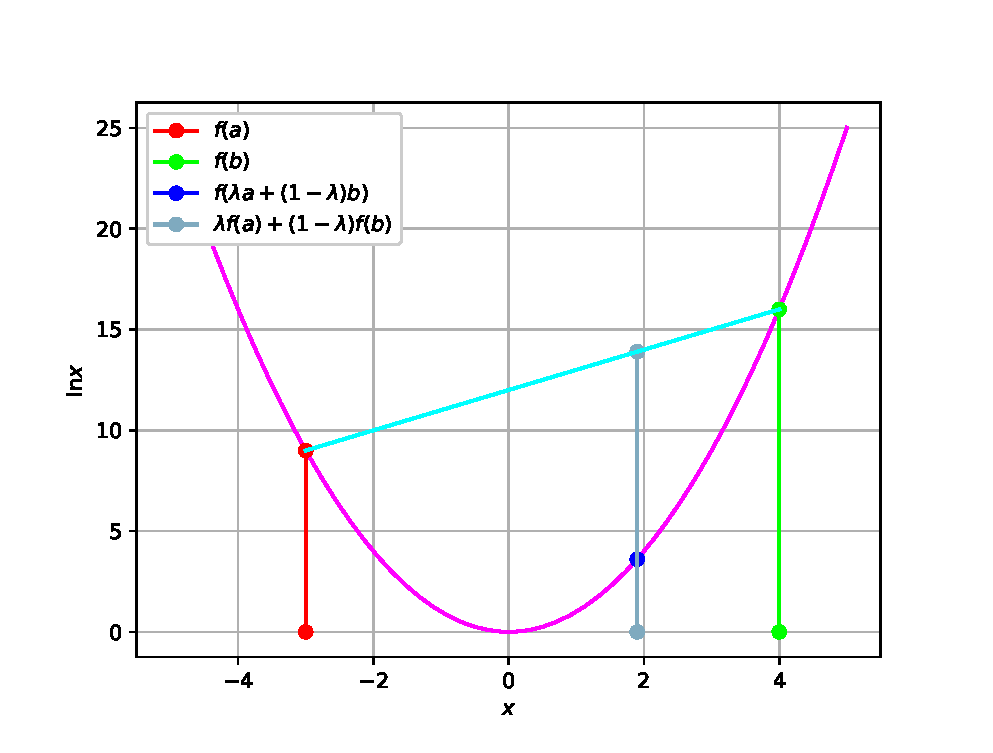
\includegraphics[width=\columnwidth]{./figs/opt/convex.eps}
\caption{ $f(\lambda)$ versus $\lambda$}.
\label{fig:conv_def}	
\end{figure}
%
\item Show that
%
\begin{align}
\label{eq:convex_def}
f\sbrak{t \lambda_1 + \brak{1-t}\lambda_2} \leq 
t f\brak{\lambda_1} + \brak{1-t}f\brak{\lambda_2}
\end{align}
%
for $\quad 0 < t < 1$.  This is true for any convex function.
%
\item Show that 
%
\begin{equation}
\eqref{eq:convex_def} \quad \implies f^{(2)}(\lambda) > 0
\end{equation}
%
\item Show that a covex function has a unique minimum.
%
\end{enumerate}
%

\section{Gradient Descent}
%\renewcommand{\theequation}{\theenumi}
%\begin{enumerate}[label=\thesubsection.\arabic*.,ref=\thesubsection.\theenumi]
%%\begin{enumerate}[label=\arabic*.,ref=\thesubsection.\theenumi]
%\numberwithin{equation}{enumi}
%

\item Find the absolute maximum and absoute minimum value of the following functions in the given intervals
%
\begin{enumerate}
\item $f(x) = 4x - \frac{1}{2}x^2, x \in \brak{-2,\frac{9}{2}}$
\item $f(x) = \brak{x-1}^2 + 3,  x \in \brak{-3,1}$
\end{enumerate}
%
\item Find the maximum profit that a company can make, if the profit function is given by
\begin{align}
p(x) = 41-72x - 18x^2
\end{align}
%
\item Find two positive numbers whose sum is 15 and the sum of whose squares is minimum.
\item Find two numbers whose sum is 24 and whose product is as large as possible.
\item Find two positive numbers whose sum is 16 and the sum of whose cubes is minimum.
\item The sum of the perimeter of a circle and square is $k$, where $k$ is some constant. Prove that the sum of their areas is least when the side of square is double the radius of the circle.
\item A window is in the form of a rectangle surmounted by a semicircular opening. The total perimeter of the window is 10 m. Find the dimensions of the window to admit maximum light through the whole opening.

\item Find the shortest distance of the point $\myvec{0\\c}$ from the parabola $y = x^2$, where $\frac{1}{2} \le c \le 5$.
\item Find the maximum area of an isosceles triangle inscribed in the ellipse 
%
\begin{align}
\vec{x}^T\myvec{a^2 & 0 \\ 0 & b^2}\vec{x} = a^2b^2
\end{align}
%
with its vertex at one end of the major axis.
\item Maximise Z=-x+2y, subject to the constraints:
x$\geq$3, x+y$\geq$5, x+2y$\geq$6, y$\geq$0.\\
\item Maximise Z=x+y, subject to x-y$\leq$-1,-x+y$\leq$0, x,y$\geq$0.\\
\item Reshma wishes to mix two types of food P and Q in such a way that the vitamin
contents of the mixture contain at least 8 units of vitamin A and 11 units of
vitamin B. Food P costs Rs 60/kg and Food Q costs Rs 80/kg. Food P contains
3 units/kg of Vitamin A and 5 units/kg of Vitamin B while food Q contains
4 units/kg of Vitamin A and 2 units/kg of vitamin B. Determine the minimum cost
of the mixture.\\
\item One kind of cake requires 200g of flour and 25g of fat, and another kind of cake
requires 100g of flour and 50g of fat. Find the maximum number of cakes which
can be made from 5kg of flour and 1 kg of fat assuming that there is no shortage
of the other ingredients used in making the cakes.\\
\item A factory makes tennis rackets and cricket bats. A tennis racket takes 1.5 hours
of machine time and 3 hours of craftman’s time in its making while a cricket bat
takes 3 hour of machine time and 1 hour of craftman’s time. In a day, the factory
has the availability of not more than 42 hours of machine time and 24 hours of
craftsman’s time.\\
(i) What number of rackets and bats must be made if the factory is to work
at full capacity?\\
(ii)If the profit on a racket and on a bat is Rs 20 and Rs 10 respectively, find
the maximum profit of the factory when it works at full capacity.\\
\item A manufacturer produces nuts and bolts. It takes 1 hour of work on machine A
and 3 hours on machine B to produce a package of nuts. It takes 3 hours on
machine A and 1 hour on machine B to produce a package of bolts. He earns a
profit of Rs17.50 per package on nuts and Rs 7.00 per package on bolts. How
many packages of each should be produced each day so as to maximise his
profit, if he operates his machines for at the most 12 hours a day?\\
\item A factory manufactures two types of screws, A and B. Each type of screw
requires the use of two machines, an automatic and a hand operated. It takes
4 minutes on the automatic and 6 minutes on hand operated machines to
manufacture a package of screws A, while it takes 6 minutes on automatic and
3 minutes on the hand operated machines to manufacture a package of screws
B. Each machine is available for at the most 4 hours on any day. The manufacturer
can sell a package of screws A at a profit of Rs 7 and screws B at a profit of
Rs 10. Assuming that he can sell all the screws he manufactures, how many
packages of each type should the factory owner produce in a day in order to
maximise his profit? Determine the maximum profit.\\
\item A cottage industry manufactures pedestal lamps and wooden shades, each
requiring the use of a grinding/cutting machine and a sprayer. It takes 2 hours on
grinding/cutting machine and 3 hours on the sprayer to manufacture a pedestal
lamp. It takes 1 hour on the grinding/cutting machine and 2 hours on the sprayer
to manufacture a shade. On any day, the sprayer is available for at the most 20
hours and the grinding/cutting machine for at the most 12 hours. The profit from
the sale of a lamp is Rs 5 and that from a shade is Rs 3. Assuming that the
manufacturer can sell all the lamps and shades that he produces, how should he
schedule his daily production in order to maximise his profit?\\
\item A company manufactures two types of novelty souvenirs made of plywood.
Souvenirs of type A require 5 minutes each for cutting and 10 minutes each for
assembling. Souvenirs of type B require 8 minutes each for cutting and 8 minutes
each for assembling. There are 3 hours 20 minutes available for cutting and 4
hours for assembling. The profit is Rs 5 each for type A and Rs 6 each for type
B souvenirs. How many souvenirs of each type should the company manufacture
in order to maximise the profit?\\
\item A merchant plans to sell two types of personal computers – a desktop model and
a portable model that will cost Rs 25000 and Rs 40000 respectively. He estimates
that the total monthly demand of computers will not exceed 250 units. Determine
the number of units of each type of computers which the merchant should stock
to get maximum profit if he does not want to invest more than Rs 70 lakhs and if
his profit on the desktop model is Rs 4500 and on portable model is Rs 5000.\\
\item A diet is to contain at least 80 units of vitamin A and 100 units of minerals. Two
foods$ F_{1}$ and $F_{2}$ are available. Food $F_{1}$ costs Rs 4 per unit food and $F_{2}$ costs
Rs 6 per unit. One unit of food $F_{1}$ contains 3 units of vitamin A and 4 units of
minerals. One unit of food $F_{2}$ contains 6 units of vitamin A and 3 units of minerals.
Formulate this as a linear programming problem. Find the minimum cost for diet
that consists of mixture of these two foods and also meets the minimal nutritional
requirements.\\
\item There are two types of fertilisers $F_{1}$ and $F_{2}$.$F_{1}$ consists of $10\%$ nitrogen and $6\%$
phosphoric acid and $F_{2}$ consists of $5\%$ nitrogen and $10\%$ phosphoric acid. After
testing the soil conditions, a farmer finds that she needs atleast 14 kg of nitrogen
and 14 kg of phosphoric acid for her crop. If $F_{1}$ costs Rs 6/kg and $F_{2}$ costs
Rs 5/kg, determine how much of each type of fertiliser should be used so that
nutrient requirements are met at a minimum cost. What is the minimum cost?\\
\item The corner points of the feasible region determined by the following system of
linear inequalities:
2x+y$\leq$10, x+3y$\leq$15, x,y$\geq$0 are (0,0), (5,0),(3,4) and (0,5).Let
Z=px+qy, where p,q$>$0.Condition on p and q so that the maximum of Z
occurs at both (3,4) and (0,5) is\\
(A) p = q\\
(B) p = 2q\\
(C) p = 3q\\
(D) q = 3p\\
\item Refer to Example 9. How many packets of each food should be used to maximise
the amount of vitamin A in the diet? What is the maximum amount of vitamin A
in the diet?\\
\item A farmer mixes two brands P and Q of cattle feed. Brand P, costing Rs 250 per
bag, contains 3 units of nutritional element A, 2.5 units of element B and 2 units
of element C. Brand Q costing Rs 200 per bag contains 1.5 units of nutritional
element A, 11.25 units of element B, and 3 units of element C. The minimum
requirements of nutrients A, B and C are 18 units, 45 units and 24 units respectively.
Determine the number of bags of each brand which should be mixed in order to
produce a mixture having a minimum cost per bag? What is the minimum cost of
the mixture per bag?\\
\item A dietician wishes to mix together two kinds of food X and Y in such a way that
the mixture contains at least 10 units of vitamin A, 12 units of vitamin B and
8 units of vitamin C. The vitamin contents of one kg food is given below:\\
\begin{tabular}{|c|c|c|c|}
\hline
\textbf{Food} &\textbf{Vitamin A} &\textbf{Vitamin B} & \textbf{VitaminC}\\
\hline
X & 1 & 2 & 3\\
\hline
Y &2 &2 &1\\
\hline


\end{tabular}\\
One kg of food X costs Rs 16 and one kg of food Y costs Rs 20. Find the least
cost of the mixture which will produce the required diet?\\
\item A manufacturer makes two types of toys A and B. Three machines are needed
for this purpose and the time (in minutes) required for each toy on the machines
is given below:\\
\begin{tabular}{|c|c|c|c|}
\hline
 \multicolumn{3}{|r}{\textbf{ Machines}}& \\ \cline{2-4}
\hline
\textbf {Types of toys}&\textbf{I}&\textbf{II}&\textbf{III}\\
\hline
A&12&18&6\\
\hline
 B&6&0&9\\
 \hline 

\end{tabular}



Each machine is available for a maximum of 6 hours per day. If the profit on
each toy of type A is Rs 7.50 and that on each toy of type B is Rs 5, show that 15
toys of type A and 30 of type B should be manufactured in a day to get maximum
profit.\\
\item An aeroplane can carry a maximum of 200 passengers. A profit of Rs 1000 is
made on each executive class ticket and a profit of Rs 600 is made on each
economy class ticket. The airline reserves at least 20 seats for executive class.
However, at least 4 times as many passengers prefer to travel by economy class
than by the executive class. Determine how many tickets of each type must be
sold in order to maximise the profit for the airline. What is the maximum profit?\\
\item Two godowns A and B have grain capacity of 100 quintals and 50 quintals
respectively. They supply to 3 ration shops, D, E and F whose requirements are
60, 50 and 40 quintals respectively. The cost of transportation per quintal from
the godowns to the shops are given in the following table:\\
\begin{tabular}{|c|c|c|}
\hline
 \multicolumn{2}{|l}{\textbf{ Transportation cost per qunital (in Rs)}}& \\ \cline{2-3}
\hline
\textbf {From/To}&\textbf{A}&\textbf{B}\\
\hline
D&6&4\\
\hline
 E&3&2\\
 \hline 
 F&2.50&3\\
 \hline

\end{tabular}\\


How should the supplies be transported in order that the transportation cost is
minimum? What is the minimum cost?\\
\item An oil company has two depots A and B with capacities of 7000 L and 4000 L
respectively. The company is to supply oil to three petrol pumps, D, E and F
whose requirements are 4500L, 3000L and 3500L respectively. The distances
(in km) between the depots and the petrol pumps is given in the following table:\\
\begin{tabular}{|c|c|c|}
\hline
 \multicolumn{2}{|l}{\textbf{Distance in (km.)}}& \\ \cline{2-3}
\hline
\textbf {From/To}&\textbf{A}&\textbf{B}\\
\hline
D&7&3\\
\hline
 E&6&4\\
 \hline 
 F&3&2\\
 \hline

\end{tabular}\\

Assuming that the transportation cost of 10 litres of oil is Re 1 per km, how
should the delivery be scheduled in order that the transportation cost is minimum?
What is the minimum cost?\\
\item A fruit grower can use two types of fertilizer in his garden, brand P and brand Q.
The amounts (in kg) of nitrogen, phosphoric acid, potash, and chlorine in a bag of
each brand are given in the table. Tests indicate that the garden needs at least
240 kg of phosphoric acid, at least 270 kg of potash and at most 310 kg of
chlorine.
If the grower wants to minimise the amount of nitrogen added to the garden,
how many bags of each brand should be used? What is the minimum amount of
nitrogen added in the garden?\\
\begin{tabular}{|c|c|c|}
\hline
 \multicolumn{2}{|r}{\textbf{ kg per bag}}& \\ \cline{1-3}
\hline
&\textbf{Brand P}&\textbf{Brand Q}\\
\hline
Nitrogen&3&3.5\\
\hline
Phospheric acid&1&2\\
\hline
Potash&3&1.5\\
\hline
Chlorine&1.5&2\\
\hline

\end{tabular}

\item Refer to Question 29. If the grower wants to maximise the amount of nitrogen
added to the garden, how many bags of each brand should be added? What is
the maximum amount of nitrogen added?\\
\item A toy company manufactures two types of dolls, A and B. Market research and
available resources have indicated that the combined production level should not
exceed 1200 dolls per week and the demand for dolls of type B is at most half of that
for dolls of type A. Further, the production level of dolls of type A can exceed three
times the production of dolls of other type by at most 600 units. If the company
makes profit of Rs 12 and Rs 16 per doll respectively on dolls A and B, how many of
each should be produced weekly in order to maximise the profit?
\item Find the shortest distance of the point $\myvec{0\\c}$ from the parabola $y = x^2$, where $\frac{1}{2} \le c \le 5$.
\item Find the maximum area of an isosceles triangle inscribed in the ellipse 
%
\begin{align}
\vec{x}^T\myvec{a^2 & 0 \\ 0 & b^2}\vec{x} = a^2b^2
\end{align}
%
with its vertex at one end of the major axis.
%\item Find the maximum and minimum values, if any, of the following functions given by 
%%
%\begin{enumerate}
%\item $f(x) = \brak{2x-1}^2+3$
%\item $f(x) = 9x^2+12x+2$
%\item $f(x) = -\brak{x-1}^2+10$
%\item $f(x) = x^2$.
%\end{enumerate}
%\item Find the absolute maximum and absoute minimum value of the following functions in the given intervals
%%
%\begin{enumerate}
%\item $f(x) = 4x - \frac{1}{2}x^2, x \in \brak{-2,\frac{9}{2}}$
%\item $f(x) = \brak{x-1}^2 + 3,  x \in \brak{-3,1}$
%\end{enumerate}
%%
%\item Find the maximum profit that a company can make, if the profit function is given by
%\begin{align}
%p(x) = 41-72x - 18x^2
%\end{align}
%%
%\item Find two positive numbers whose sum is 15 and the sum of whose squares is minimum.
%\item Find two numbers whose sum is 24 and whose product is as large as possible.
%\item Find two positive numbers whose sum is 16 and the sum of whose cubes is minimum.
%\item The sum of the perimeter of a circle and square is $k$, where $k$ is some constant. Prove that the sum of their areas is least when the side of square is double the radius of the circle.
%\item A window is in the form of a rectangle surmounted by a semicircular opening. The total perimeter of the window is 10 m. Find the dimensions of the window to admit maximum light through the whole opening.
\item  \textbf{(Manufacturing problem)} A manufacturing company makes two models
A and B of a product. Each piece of Model A requires 9 labour hours for fabricating
and 1 labour hour for finishing. Each piece of Model B requires 12 labour hours for
fabricating and 3 labour hours for finishing. For fabricating and finishing, the maximum
labour hours available are 180 and 30 respectively. The company makes a profit of
Rs 8000 on each piece of model A and Rs 12000 on each piece of Model B. How many
pieces of Model A and Model B should be manufactured per week to realise a maximum
profit? What is the maximum profit per week?\\
\item \textbf {(Diet problem)} A dietician has to develop a special diet using two foods
P and Q. Each packet (containing 30 g) of food P contains 12 units of calcium, 4 units
of iron, 6 units of cholesterol and 6 units of vitamin A. Each packet of the same quantity
of food Q contains 3 units of calcium, 20 units of iron, 4 units of cholesterol and 3 units
of vitamin A. The diet requires atleast 240 units of calcium, atleast 460 units of iron and
at most 300 units of cholesterol. How many packets of each food should be used to
minimise the amount of vitamin A in the diet? What is the minimum amount of vitamin A?\\


%\end{enumerate}
%\end{document}

\section{Lagrange Multipliers}
\renewcommand{\theequation}{\theenumi}
\begin{enumerate}[label=\thesubsection.\arabic*.,ref=\thesubsection.\theenumi]
\numberwithin{equation}{enumi}

\item
	\label{convex_code}
Find
\begin{align}
\label{eq:opt_line_nor_h}
	\min_{\mbf{x}}g\brak{\mbf{x}} = \norm{\vec{x}-\vec{P}}^2 = r^2 \\
\text{s.t.} \quad 	h\brak{\mbf{x}} = \vec{n}^T\vec{x} - c = 0\label{eq2_1_line}
%	\quad g\brak{\mbf{x}} = x_1 + x_2 - 9 = 0
\end{align}
by plotting the circles $g\brak{\vec{x}}$
%
%\begin{equation}
% \norm{\vec{x}-\myvec{8\\6}}^2 =r^2
%%(x_1-8)^2 + (x_2-6)^2 = r^2
%\end{equation}
%
% $\mbf{x}= \myvec{x_1\\x_2}$, 
for different values of $r$ along with the line $g\brak{\mbf{x}}$.
%
%\begin{equation}
%\label{eq2_1_line}
%g\brak{\mbf{x}} = \myvec{1 & 1}\vec{x} - 9 = 0
%\end{equation} 
%
\\
\solution 
The following code plots Fig. \ref{fig:concirc}	

%	
\begin{lstlisting}
codes/opt/concirc.py
\end{lstlisting}

%
\begin{figure}[!ht]
\centering
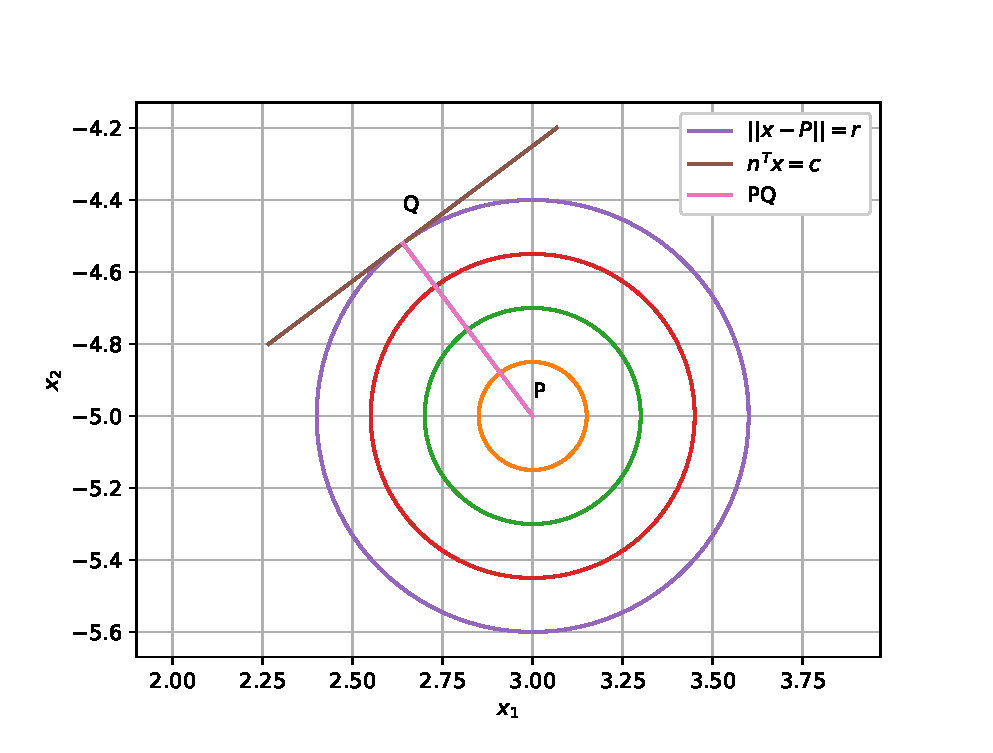
\includegraphics[width=\columnwidth]{./figs/opt/concirc.eps}
\caption{ Finding $ \displaystyle \min_{\mbf{x}}g\brak{\mbf{x}}$}.
\label{fig:concirc}	
\end{figure}
%
\item By solving the quadratic equation obtained from \eqref{eq:opt_line_nor_h},
show that 
\label{prob:minr}
\begin{align}
\min_{\vec{x}} r = \frac{3}{5}, \vec{x}_{\min} = \vec{Q}  = \myvec{2.64\\-4.52}
\end{align}
%
%and find $,
%$ that minimizes $r$. By labeling  $\vec{Q}$ 
In Fig. \ref{fig:concirc}, it can be seen  that $\vec{Q}$ is the point of contact of the line $L$ with the circle of minimum radius $r = \frac{3}{5}$.
%Obtain a theoretical solution for problem \ref{convex_code} 
%%using coordinate geometry.
%
%\solution 
%From \eqref{eq2_1_line} and \eqref{eq2_1_circ}, 
%%
%\begin{align}
%r^2 & = (x_1-8)^2 + (3- x_1)^2 \\
%&= 2 x_1^2 - 22 x_1 + 73 \\
%\Rightarrow r^2 &= \frac{\brak{2x_1-11}^2 + 5^2}{2}
%\end{align}
%%
%which is minium when $x_1 = \frac{11}{2}, x_2 = \frac{7}{2}$.  The minimum value is $\frac{25}{2}$ and 
%the radius $r = \frac{5}{\sqrt{2}}$.
\item Show that 
\begin{align}
\label{eq:lagrange_n}
\nabla h(\vec{x}) =  \myvec{3 \\ -4} = \vec{n}
\end{align}
where
\begin{equation}
\nabla =  
\begin{pmatrix}
\frac{\partial}{\partial x_1} \\
\frac{\partial}{\partial x_2} 
\end{pmatrix}
\end{equation}

\item Show that 
\begin{align}
\nabla g(\vec{x}) = 2\cbrak{\vec{x}-\myvec{3 \\ -5}} = 2\cbrak{\vec{x}-\vec{P}}
\label{eq:lagrange_pq}
\end{align}
%
%is the direction vector of the normal at $\vec{x}$.
\item From Fig. \ref{fig:concirc}, show that 
\begin{align}
\label{eq:opt_normal}
\nabla g(\vec{Q}) = \lambda \nabla h(\vec{Q}),
\end{align}
%
\solution In Fig. \ref{fig:concirc}, PQ is the normal to the line $L$, represented by $h\brak{\vec{x}}$. 
$\because$ the normal vector of $L$ is in the same direction as $PQ$,  for some constant $k$, 
%
\begin{align}
%\label{eq:opt_normal}
\brak{\vec{Q}-\vec{P}} = k \vec{n}
\end{align}
%
which is the same as \eqref{eq:opt_normal} after substituting from \eqref{eq:lagrange_n}.
 and \eqref{eq:lagrange_pq}.
%where $\vec{p}$ is the point of contact.
\item Use \eqref{eq:opt_normal} and $\vec{h(\vec{Q})}=0$ from \eqref{eq2_1_line} to obtain $\vec{Q}$.
\\
\solution From the given equations, we obtain
\begin{align}
\brak{\vec{Q}-\vec{P}}-\lambda \vec{n} &= 0 
\\
\vec{n}^T\vec{Q} - c &= 0
\label{eq:lagrange_mat_eq}
\end{align}
%
which can be simplifed to obtain
%
\begin{align}
\myvec{\vec{I} & -\vec{n} \\ \vec{n}^T & 0}\myvec{\vec{Q}\\ \lambda} = \myvec{\vec{P}\\c}
%\vec{Q} = \vec{P}+\frac{\brak{c-\vec{n}^T\vec{P}}}{\norm{\vec{n}}^2}\vec{n}
\label{eq:lagrange_mat_sol}
\end{align}
The following code computes the solution to \eqref{eq:lagrange_mat_sol}
%
\begin{lstlisting}
codes/opt/lagmul.py
\end{lstlisting}

\item
\label{lagrange}
	Define 
	\begin{equation}
	\label{lagrangian}
	C\brak{\mbf{x},\lambda} = g\brak{\mbf{x}} - \lambda h\brak{\mbf{x}}%, \quad \lambda > 0
	\end{equation}
and show that $\vec{Q}$ can also be obtained by 
solving the equations
%
\begin{align}
\nabla C\brak{\mbf{x},\lambda} &= 0.
\label{tangent}
\end{align}
%
What is the sign of $\lambda$?  $C$ is known as the Lagrangian and the above technique is known as the Method of Lagrange Multipliers.

%\solution
%From \eqref{eq2_1_line} and \eqref{eq2_1_circ}, 
%%
%\begin{align}
%L\brak{\mbf{x},\lambda} &= (x_1-8)^2 + (x_2-6)^2 - \lambda \brak{x_1 + x_2 - 9} \\
%\Rightarrow \nabla L\brak{\mbf{x},\lambda}  & = 
%\begin{pmatrix}
%2x_1  - 16 - \lambda \\
%2x_2 - 12 - \lambda \\
%x_1 + x_2 -9
%\end{pmatrix}
%\\
%&=
%\begin{pmatrix}
%2 &0 & - 1 \\
%0 &2 & - 1 \\
%1 & 1 & 0 
%\end{pmatrix}
%\begin{pmatrix}
%x_1 \\
%x_2 \\
%\lambda
%\end{pmatrix}
%= 
%\begin{pmatrix}
%16 \\
% 12 \\
%9
%\end{pmatrix}
%=
%0 
%\\
%\Rightarrow 
%\begin{pmatrix}
%x_1 \\
%x_2 \\
%\lambda
%\end{pmatrix}
%&= 
%\begin{pmatrix}
%\frac{11}{2} \\
% \frac{7}{2} \\
%-5
%\end{pmatrix}
%\end{align}
%%
%using the following python script.  Note that this method yields the same result as the previous exercises.  Thus, $\lambda$ is negative.
%	
\item Obtain $\vec{Q}$ using gradient descent.
\\
\solution
\begin{lstlisting}
codes/opt/gd_lagrange.py
\end{lstlisting}

\end{enumerate}

\section{Quadratic Programming}
\renewcommand{\theequation}{\theenumi}
\begin{enumerate}[label=\arabic*.,ref=\thesection.\theenumi]
\numberwithin{equation}{enumi}

\item An apache helicopter of the enemy is flying along the curve given by 
	\label{prob:dist_pt_parab}
\begin{align}
\label{eq:dist_pt_parab}
y = x^2 +7
\end{align}
%
A soldier, placed at 
\begin{align}
\vec{P} = \myvec{3\\7}.  
\end{align}
%
wants to shoot the heicopter when it is nearest to him.  Express this as an optimization problem.
%\item
%Express the problem of 
%finding the point on the curve 
%\begin{align}
%\label{eq:dist_pt_parab}
%x^2 = 2y
%\end{align}
%%
%nearest to the point 
%\begin{align}
%\vec{P} = \myvec{0\\5}.  
%\end{align}
%%
%as an optiimization problem.
\\
\solution The given problem can be expressed as
\begin{align}
\label{eq:qp_dist_pt_parab}
\min_{\vec{x}}\norm{\vec{x}-\vec{P}}^2
\\
\text{s.t. }\vec{x}^T\vec{V}\vec{x} + \vec{u}^T\vec{x}  +d = 0
\end{align}
%
where
%
\begin{align}
\vec{V} &= \myvec{1 & 0\\0 & 0}
\\
\vec{u} &= -\myvec{0 \\ 1}
\\
d &= 7
\end{align}
\item Show that the constraint in \ref{eq:qp_dist_pt_parab} is nonconvex.
\item Show that the following {\em relaxation} makes \eqref{eq:qp_dist_pt_parab} a convex optimization problem.
%
\begin{align}
\label{eq:qp_dist_pt_parab_conv}
\min_{\vec{x}}\brak{\vec{x}-\vec{P}}^T\brak{\vec{x}-\vec{P}}
\\
\text{s.t. }\vec{x}^T\vec{V}\vec{x} + \vec{u}^T\vec{x}  \le 0
\end{align}
%
%
\item Solve \eqref{eq:qp_dist_pt_parab_conv} using cvxpy.
\\
\solution  The following code yields the minimum distance as 2.236 and the nearest point on the curve as
%
\begin{align}
\vec{Q} &= \myvec{1\\8}
\end{align}

\begin{lstlisting}
codes/qp_cvx.py
\end{lstlisting}

\item Solve \eqref{eq:qp_dist_pt_parab_conv} using the method of Lagrange multipliers.
\item Graphically verify the solution to Problem \ref{prob:dist_pt_parab}. 
%by drawing a figure.
\\
\solution 
The following code plots Fig. \ref{fig:qp_parab}
%	
\begin{lstlisting}
codes/qp_parab.py
\end{lstlisting}

%
\begin{figure}[!ht]
\centering
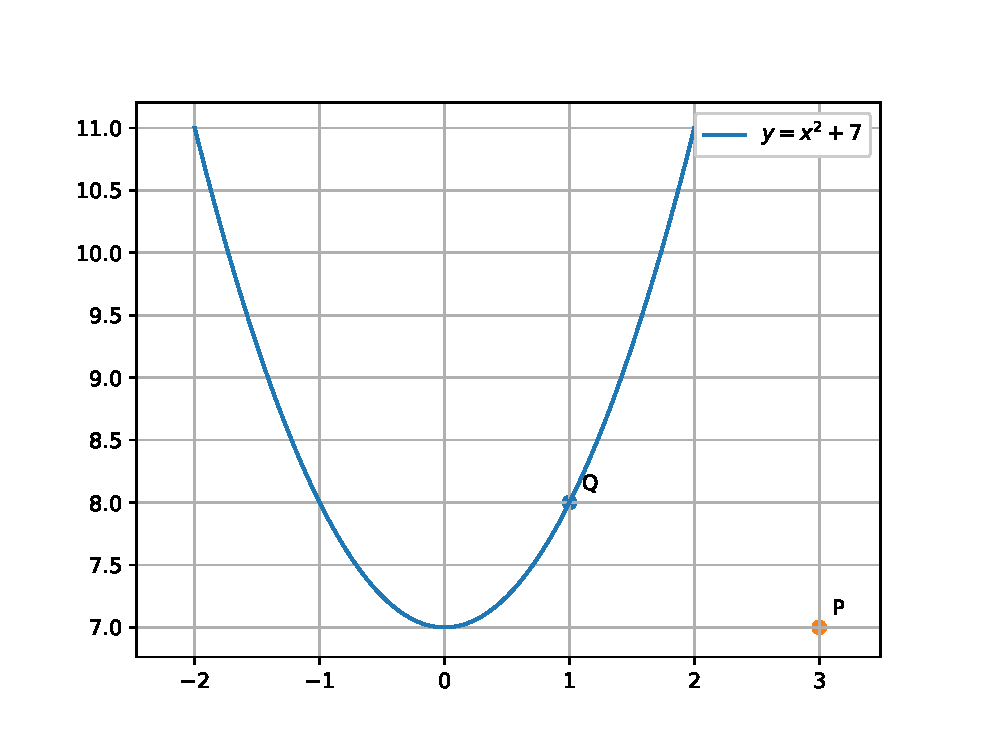
\includegraphics[width=\columnwidth]{./figs/qp_parab.eps}
\caption{ $\vec{Q}$ is closest to $\vec{P}$}.
\label{fig:qp_parab}
\end{figure}
%
%\item Frame 	
% as an optimization problem.
%\label{prob:qp_dist_pt_parab}
%\\
%
%\solution 
%From \eqref{eq2_1_line} and \eqref{eq2_1_circ}, 
%%
%\begin{align}
%r^2 & = (x_1-8)^2 + (3- x_1)^2 \\
%&= 2 x_1^2 - 22 x_1 + 73 \\
%\Rightarrow r^2 &= \frac{\brak{2x_1-11}^2 + 5^2}{2}
%\end{align}
%%
%which is minium when $x_1 = \frac{11}{2}, x_2 = \frac{7}{2}$.  The minimum value is $\frac{25}{2}$ and 
%the radius $r = \frac{5}{\sqrt{2}}$.
%	
%\begin{lstlisting}
%codes/optimization/lagmul.py
%\end{lstlisting}
\item Solve \eqref{eq:qp_dist_pt_parab_conv} using gradient descent.
%
\end{enumerate}

\section{Semi Definite Programming}
\renewcommand{\theequation}{\theenumi}
\begin{enumerate}[label=\arabic*.,ref=\thesection.\theenumi]
\numberwithin{equation}{enumi}

%\item An apache helicopter of the enemy is flying along the curve given by 
%	\label{prob:dist_pt_parab_sdp}
%\begin{align}
%\label{eq:dist_pt_parab_sdp}
%y = x^2 +7
%\end{align}
%%
%A soldier, placed at 
%\begin{align}
%\vec{P} = \myvec{3\\7}.  
%\end{align}
%%
%wants to shoot the heicopter when it is nearest to him.  Express this as an optimization problem.
\item
	\label{prob:dist_pt_parab_sdp}
Express the problem of 
finding the point on the curve 
\begin{align}
\label{eq:dist_pt_parab_sdp}
x^2 = 2y
\end{align}
%
nearest to the point 
\begin{align}
\vec{P} = \myvec{0\\5}.  
\end{align}
%
as an optimization problem.
\\
\solution The given problem can be expressed as
%
\begin{align}
\label{eq:qp_dist_pt_parab_sdp_qp}
\min_{\vec{x}}\vec{x}^T\vec{Q}_0\vec{x}+\vec{q}_0^T\vec{x}+c_0
\\
\text{s.t. }\vec{x}^T\vec{Q}_1\vec{x} + \vec{q}_1^T\vec{x} +c_1 \le 0
\end{align}
%
%where $\vec{V} \succeq 0$.
%\begin{align}
%\label{eq:qp_dist_pt_parab_sdp}
%\begin{split}
%\min_{\vec{x}}\vec{X}^T\myvec{\vec{I} & \vec{0} \\ \vec{0} & \vec{0}}\vec{X}-2\myvec{\vec{P}^T & \vec{0}}\vec{X}+\norm{\vec{P}}^2
%\\
%\text{s.t. }\vec{x}^T\vec{V}\vec{x} + \vec{u}^T\vec{x}  = 0
%\end{split}
%\end{align}
%
where
%
\begin{align}
\vec{Q}_0 &= \vec{I}, \vec{Q}_1 = \myvec{1 & 0\\0 & 0}
\\
\vec{q}_0 &=-2\vec{P}, \vec{q}_1 = -2\myvec{0 \\ 1}
\\
c_0 &= \norm{\vec{P}}^2, c_1 = 0
\end{align}
%\item Show that the constraint in 	
%%\label{prob:dist_pt_parab_sdp}
%\eqref{eq:qp_dist_pt_parab_sdp} is nonconvex.
%
\item Show that \eqref{eq:qp_dist_pt_parab_sdp_qp} is equivalent to
\begin{align}
\label{eq:qp_dist_pt_parab_sdp_conv}
\begin{split}
\min_{\vec{x},\theta}\theta
\\
\text{s.t. } \myvec{\vec{I} & \vec{M}_0\vec{x} \\ \vec{x}^T\vec{M}_0^T & -c_0-q_0^T\vec{x}+\theta} &\succeq 0
\\
\myvec{\vec{I} & \vec{M}_1\vec{x} \\ \vec{x}^T\vec{M}_1^T & -c_1-q_1^T\vec{x}} &\succeq 0
\end{split}
\end{align}
%
%\item Show that the following {\em relaxation} makes \eqref{eq:qp_dist_pt_parab_sdp} a convex optimization problem.
%%
%\begin{align}
%\label{eq:qp_dist_pt_parab_sdp_conv}
%\min_{\vec{x}}\brak{\vec{x}-\vec{P}}^T\brak{\vec{x}-\vec{P}}
%\\
%\text{s.t. }\vec{x}^T\vec{V}\vec{x} + \vec{u}^T\vec{x}  \le 0
%\end{align}
%
where
\begin{align}
\vec{Q}_i = \vec{M}_i^T\vec{M}_i, i = 0, 1
\end{align}
%
\item Solve \eqref{eq:qp_dist_pt_parab_sdp_conv} using cvxpy.
\item Graphically verify the solution to Problem \ref{prob:dist_pt_parab_sdp}. 
%\\
%\solution  The following code yields the minimum distance as 2.236 and the nearest point on the curve as
%%
%\begin{align}
%\vec{Q} &= \myvec{1\\8}
%\end{align}
%
%\begin{lstlisting}
%codes/qp_cvx.py
%\end{lstlisting}

\item Solve \eqref{eq:qp_dist_pt_parab_sdp_qp} using the method of Lagrange multipliers.
%by drawing a figure.
%\\
%\solution 
%The following code plots Fig. \label{fig:qp_parab_sdp}
%%	
%\begin{lstlisting}
%codes/qp_parab.py
%\end{lstlisting}
%
%%
%\begin{figure}[!ht]
%\centering
%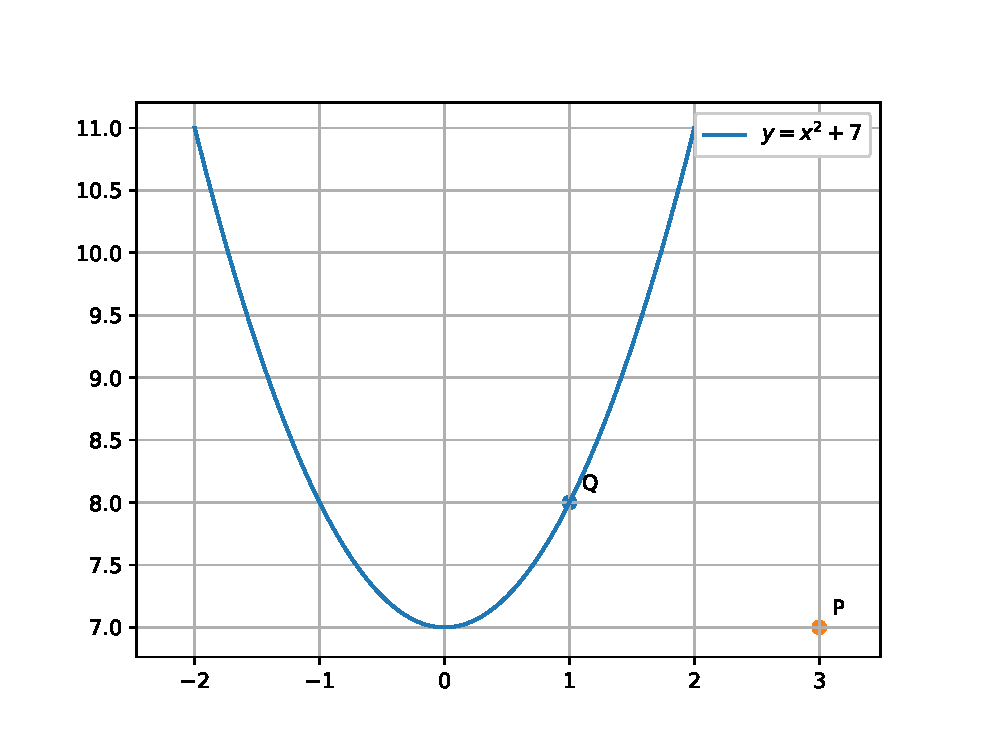
\includegraphics[width=\columnwidth]{./figs/qp_parab.eps}
%\caption{ $\vec{Q}$ is closest to $\vec{P}$}.
%\label{fig:qp_parab_sdp}
%\end{figure}
%
%\item Frame 	
% as an optimization problem.
%\label{prob:qp_dist_pt_parab}
%\\
%
%\solution 
%From \eqref{eq2_1_line} and \eqref{eq2_1_circ}, 
%%
%\begin{align}
%r^2 & = (x_1-8)^2 + (3- x_1)^2 \\
%&= 2 x_1^2 - 22 x_1 + 73 \\
%\Rightarrow r^2 &= \frac{\brak{2x_1-11}^2 + 5^2}{2}
%\end{align}
%%
%which is minium when $x_1 = \frac{11}{2}, x_2 = \frac{7}{2}$.  The minimum value is $\frac{25}{2}$ and 
%the radius $r = \frac{5}{\sqrt{2}}$.
%	
%\begin{lstlisting}
%codes/optimization/lagmul.py
%\end{lstlisting}
%\item Solve \eqref{eq:qp_dist_pt_parab_sdp_conv} using gradient descent.
%
\end{enumerate}

\section{Linear Programming}
\renewcommand{\theequation}{\theenumi}
\begin{enumerate}[label=\arabic*.,ref=\thesection.\theenumi]
\numberwithin{equation}{enumi}
%
\item Solve
\label{prob:lp_std}
\begin{align}
\max_{\vec{x}} Z &= \myvec{4 & 1}\vec{x}
\\
s.t. \quad 
\myvec{
1 & 1
\\
3 & 1
}
\vec{x} &\preceq \myvec{50\\90}
\\
\vec{x} &\succeq \vec{0}
\end{align}
%
using cvxpy.
\\
\solution The given problem can be expressed in general as
\begin{align}
\max_{\vec{x}} &\vec{c}^{T}\vec{x}
\\
s.t. \quad \vec{A}\vec{x} &\le \vec{b},
\\
\vec{x} &\succeq\vec{0}
\end{align}
%
where
\begin{align}
\vec{c} &= \myvec{4 \\ 1}
\\
\vec{A} &=
\myvec{
1 & 1
\\
3 & 1
}
\\
\vec{b}&=\myvec{50\\90}
%
\end{align}
%
and can be solved using {\em cvxpy} through the following code
\begin{lstlisting}
codes/lp_cvx.py
\end{lstlisting}
%
to obtain
\begin{align}
\vec{x} = \myvec{30\\0}, Z = 120
\end{align}
%
\item Graphically, show that the {feasible region} in  Problem \ref{prob:lp_std} result in the interior of a convex polygon and the optimal point is one of the vertices.
\solution The following code plots Fig. \ref{fig:lp_feas_reg}.
%
\begin{lstlisting}
codes/lp_cvx.py
\end{lstlisting}
%
\begin{figure}[!ht]
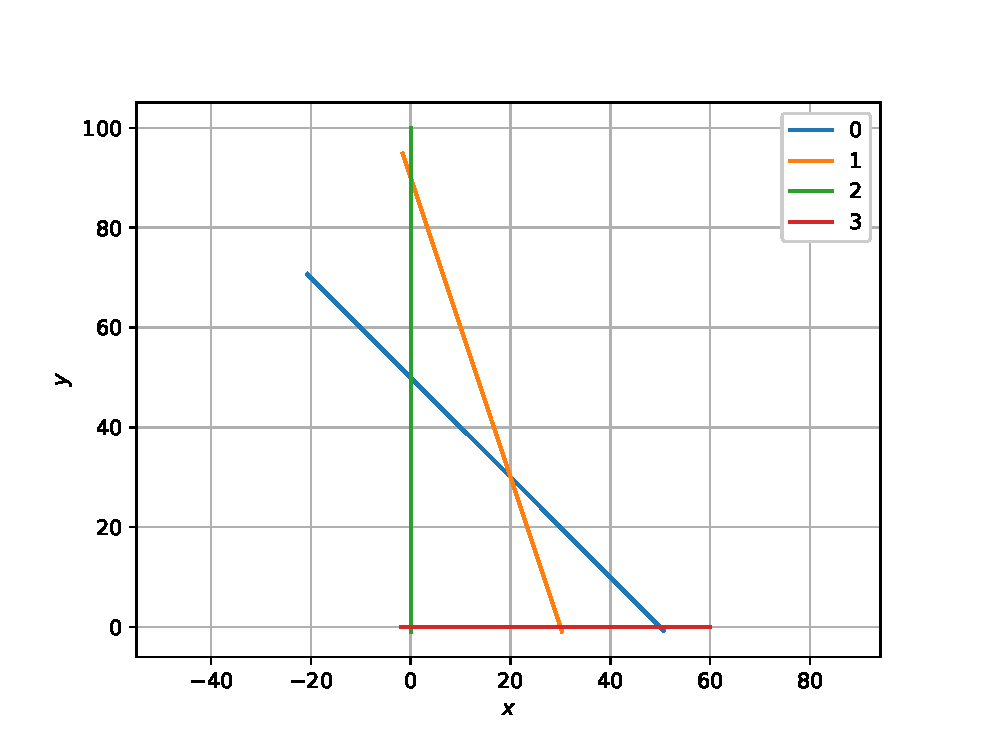
\includegraphics[width=\columnwidth]{./figs/lp_feas_reg.eps}
\caption{}
\label{fig:lp_feas_reg}
\end{figure}

%Verify the solution to graphically.
\item Solve
\begin{align}
\min_{\vec{x}} Z &= \myvec{3 & 9}\vec{x}
\\
s.t. \quad 
\myvec{
1 & 3
\\
-1 & -1
\\
1 & -1
}
\vec{x} &\preceq \myvec{60\\-10\\0}
\\
\vec{x} &\succeq \vec{0}
\label{eq:lp_exam_mult}
\end{align}
\solution The following code
\begin{lstlisting}
codes/lp_cvx_mult.py
\end{lstlisting}
%
is used to obtain
\begin{align}
\vec{x} = \myvec{15\\15}, Z = 180
\end{align}
%
%\item Write a program to plot the constraints for any linear program.

%The region in \eqref{eq:lp_constr} is shown in Fig. \ref{}
\item Solve
\begin{align}
\min_{\vec{x}} Z &= \myvec{-50 & 20}\vec{x}
\\
s.t. \quad 
\myvec{
-2 & 1
\\
-3 & -1
\\
2 & -3
}
\vec{x} &\preceq \myvec{5\\-3\\12}
\\
\vec{x} &\succeq \vec{0}
\end{align}
%
\solution The following code 
\begin{lstlisting}
codes/lp_cvx_nosol.py
\end{lstlisting}
%
shows that the given problem has no solution.
\item Verify all the above solutions using Lagrange multipliers.
\item Repeat the above exercise using the Simplex method.
\item\textbf {(Diet problem)}: A dietician wishes to mix two types of foods in such a
way that vitamin contents of the mixture contain atleast 8 units of vitamin A and 10
units of vitamin C. Food ‘I’ contains 2 units/kg of vitamin A and 1 unit/kg of vitamin C.
Food ‘II’ contains 1 unit/kg of vitamin A and 2 units/kg of vitamin C. It costs
Rs 50 per kg to purchase Food ‘I’ and Rs 70 per kg to purchase Food ‘II’. Formulate
this problem as a linear programming problem to minimise the cost of such a mixture.
\\
\solution Let the mixture contain $x$ kg of food I and $y$ kg of food II.
\\
\begin{table}[!h]
\begin{tabular}{|l|l|l|l|}
\hline
\multirow{2}{*}{Resources} & \multicolumn{2}{l|}{Food} & \multirow{2}{*}{Requirement} \\ \cline{2-3}
                           & I           & II          &                              \\ \hline
Vitamin A                  & 2           & 1           & Atleast 8 Units              \\ \hline
Vitamin C                  & 1           & 2           & Atleast 10 Units             \\ \hline
Cost                       & 50          & 70          &                              \\ \hline
\end{tabular}
\end{table}
%
The given problem can be expressed as
%GOAL: We need to minimize the cost of mixture.\\
%Cost of FOOD I per kg = Rs 50 \\
%Cost of FOOD II per kg = Rs 70 \\
% Minimize $ Z = 50x +70y$\\
% Subject to constraints:\\
% $2x+y>=8$\\
% $x+2y>=10$\\
% $x,y>=0$\\
\begin{align}
\min_{\vec{x}} Z &= \myvec{50 & 70}\vec{x}
\\
s.t. \quad 
\myvec{
2 & 1
\\
1 & 2
%\\
%2 & -3
}
\vec{x} & \succeq \myvec{8\\10}
%\preceq \myvec{5\\-3\\12}
\\
\vec{x} &\succeq \vec{0}
\label{eq:diet}
\end{align}
%
The corner points of the feasible region are available in Table \ref{table:diet_corner_pt} and plotted in Fig. \ref{fig:diet}.
%
\begin{table}[!h]
\begin{tabular}{|l|l|l|l|}
\hline
Corner Point &  $Z=50x+70y$\\
\hline
(0,8)& 560\\
\hline
(2,4)& 380\\
\hline
(10,0)& 500\\
\hline
\end{tabular}
\caption{}
\label{table:diet_corner_pt}
\end{table}
  \begin{figure}[!h]

  \centering
  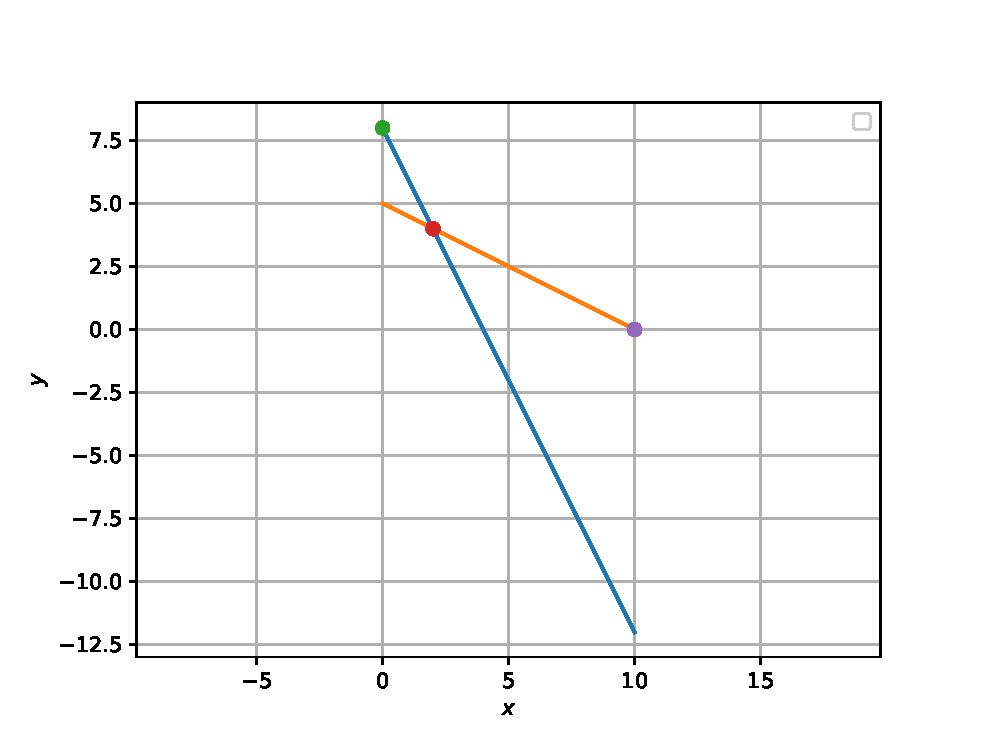
\includegraphics[width=1\linewidth]{./figs/lp_diet.eps}
\caption{}
\label{fig:diet}
  \end{figure}


The smallest value of Z is 380 at the point (2,4). But the feasible region is unbounded therefore we draw the graph of the inequality
\begin{align}
50x +70y<380
\end{align}
to check whether the resulting open half has any point common with the feasible region but on checking it doesn't have any points in common. 
Thus the minimum value of Z is 380 attained at $\myvec{2\\4}$. Hence optimal mixing strategy for the dietician would be to mix 2 Kg of Food I and 4 Kg of Food II.  The following code provides the solution to \eqref{eq:diet}.
%
\begin{lstlisting}
codes/diet.py
\end{lstlisting}



\item \textbf{(Allocation problem)} A cooperative society of farmers has 50 hectare
of land to grow two crops X and Y. The profit from crops X and Y per hectare are
estimated as Rs 10,500 and Rs 9,000 respectively. To control weeds, a liquid herbicide
has to be used for crops X and Y at rates of 20 litres and 10 litres per hectare. Further,
no more than 800 litres of herbicide should be used in order to protect fish and wild life
using a pond which collects drainage from this land. How much land should be allocated
to each crop so as to maximise the total profit of the society?\\
\solution The given problem can be formulated as
\begin{align}
\max_{\vec{x}} Z &= \myvec{10500 & 9000}\vec{x}
\\
s.t. \quad 
\myvec{
20 & 10
}
\vec{x} & \preceq 800
\\
\myvec{
1 & 1
} 
\vec{x} &= 50
\label{eq:allocation}
\end{align}
Fig  \ref{fig:allocation}
shows the intersection of various lines and the optimal point as indicated.
\begin{figure}[h]
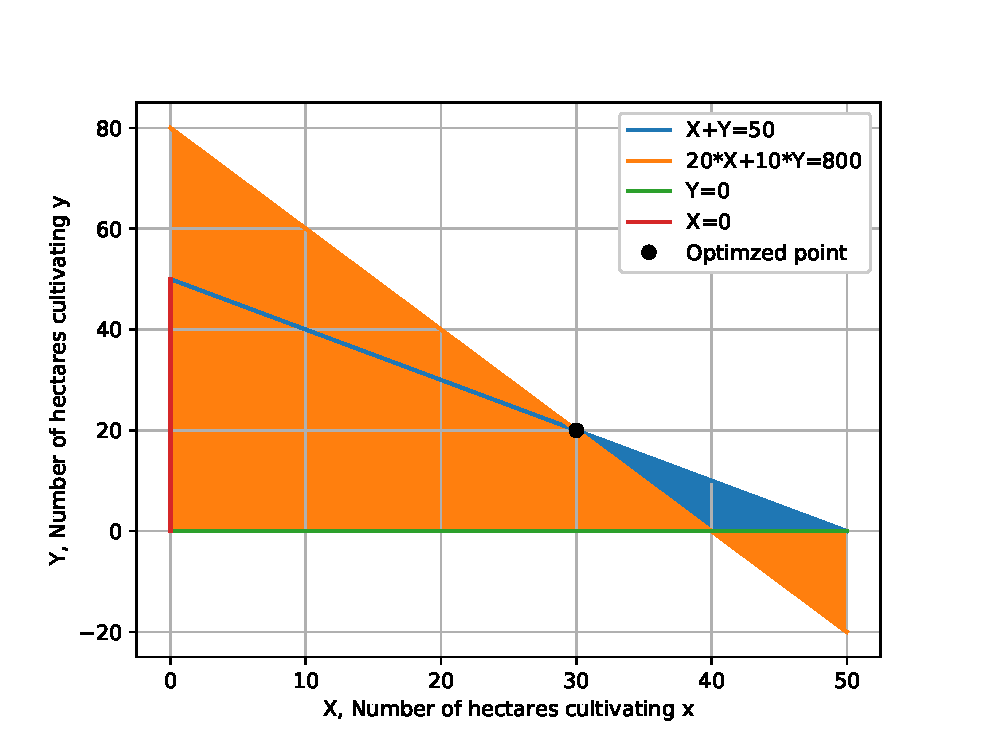
\includegraphics[width=\columnwidth]{./figs/lp_allocation.eps}
\caption{Feasible region for allocation Problem}
\caption{}
\label{fig:allocation}
\end{figure}

The following code provides the solution to \eqref{eq:allocation} at \myvec{30\\20}.
%
\begin{lstlisting}
codes/allocation.py
\end{lstlisting}

\item \textbf{(Manufacturing problem)} A manufacturer has three machines I, II
and III installed in his factory. Machines I and II are capable of being operated for
at most 12 hours whereas machine III must be operated for atleast 5 hours a day. She
produces only two items M and N each requiring the use of all the three machines.
The number of hours required for producing 1 unit of each of M and N on the three
machines are given in the following table:\\

\begin{tabular}{|c|c|c|c|}
\hline
 \multicolumn{3}{|l}{\textbf{ Number of hours required on machines}}& \\ \cline{2-4}
\hline
\textbf {Items}&\textbf{I}&\textbf{II}&\textbf{III}\\
\hline
M&1&2&1\\
\hline
 N&2&1&1.25\\
 \hline 

\end{tabular}

She makes a profit of Rs 600 and Rs 400 on items M and N respectively. How many
of each item should she produce so as to maximise her profit assuming that she can sell
all the items that she produced? What will be the maximum profit?
\\
\solution The given problem can be formulated as
\begin{align}
\max_{\vec{x}} Z &= \myvec{80000&12000}\vec{x}
\\
s.t. \quad 
\myvec{
3 & 4
\\
1 & 3
}
\vec{x} & \preceq \myvec{60\\30}
\label{eq:manufacturing}
\end{align}

Fig  \ref{fig:manufacturing}
shows the intersection of various lines and the optimal point as indicated.
\begin{figure}[h]
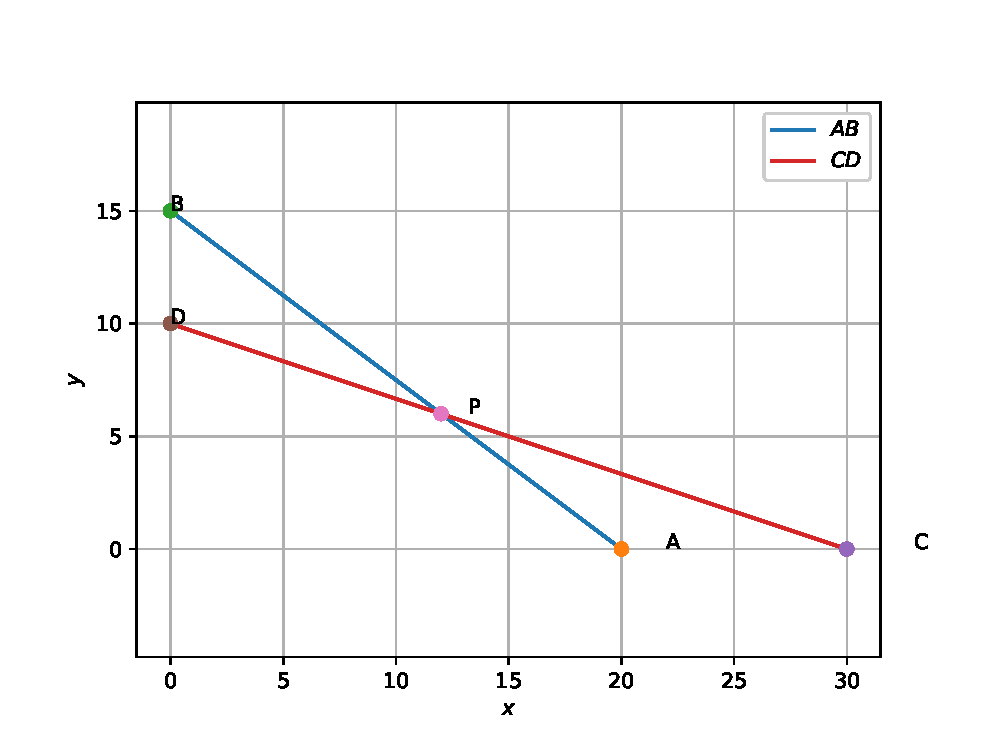
\includegraphics[width=\columnwidth]{./figs/lp_manufacturing.eps}
\caption{Feasible region for manufacturing Problem}
\caption{}
\label{fig:manufacturing}
\end{figure}

The following code provides the solution to \eqref{eq:manufacturing} at \myvec{12\\6}.
%
\begin{lstlisting}
codes/Manufacturing.py
\end{lstlisting}

\item \textbf{(Transportation problem)} There are two factories located one at
place P and the other at place Q. From these locations, a certain commodity is to be
delivered to each of the three depots situated at A, B and C. The weekly requirements
of the depots are respectively 5, 5 and 4 units of the commodity while the production
capacity of the factories at P and Q are respectively 8 and 6 units. The cost of transportation per unit is given below where A,B,C are cost in ruppes:\\
\begin{tabular}{|c|c|c|c|}
\hline
From/To & A & B & C\\
\hline
P & 160 & 100 & 150\\
\hline
Q & 100 &120 & 100\\
\hline
\end{tabular}\\
How many units should be transported from each factory to each depot in order that
the transportation cost is minimum. What will be the minimum transportation cost?
\\
\solution The given problem can be formulated as
\begin{align}
\min_{\vec{x}} Z &= \myvec{10 & -70}\vec{x}
\\
s.t. \quad 
\myvec{
1 & 1
\\
-1 & -1
}
\vec{x} & \preceq \myvec{8\\-4}
\\
\vec{x} &\preceq \myvec{5\\5}
\label{eq:transport}
\end{align}

Fig  \ref{fig:transport}
shows the intersection of various lines and the optimal point indicated as OPT PT.
\begin{figure}[h]
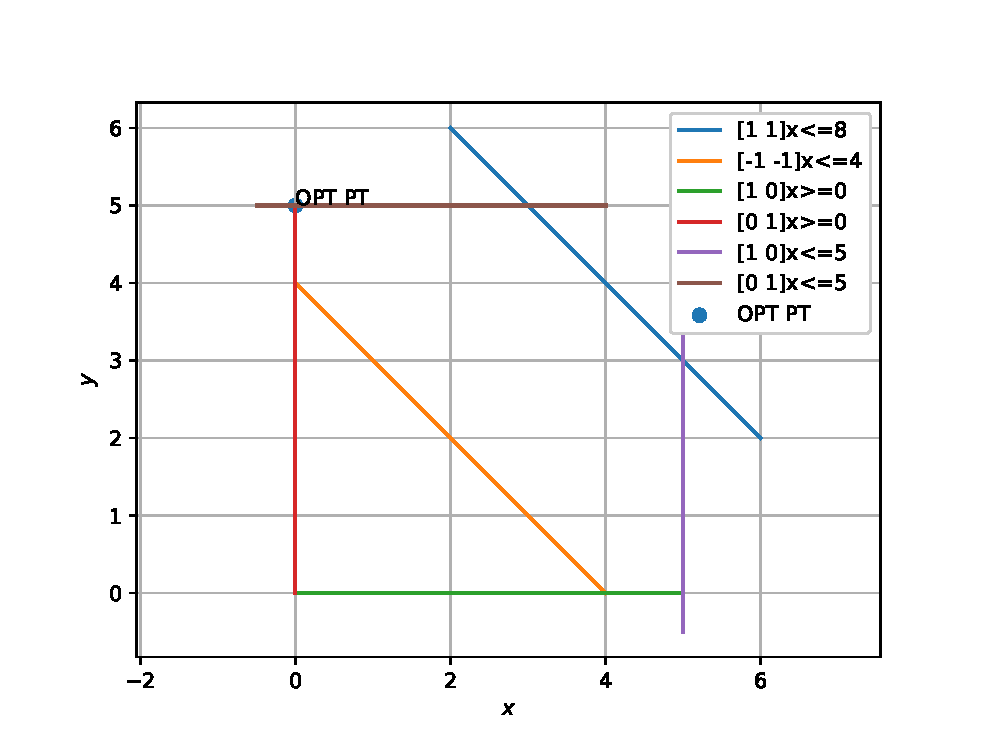
\includegraphics[width=\columnwidth]{./figs/lp_transport.eps}
\caption{Feasible region for Transportation Problem}
\caption{}
\label{fig:transport}
\end{figure}

The following code provides the solution to \eqref{eq:transport} at \myvec{0\\5}.
%
\begin{lstlisting}
codes/Transportation.py
\end{lstlisting}





\end{enumerate}
%    \end{document}
    

\section{Exercises}
\renewcommand{\theequation}{\theenumi}
\begin{enumerate}[label=\arabic*.,ref=\thesection.\theenumi]
\numberwithin{equation}{enumi}

\item Solve
\begin{align}
\min_{\vec{x}} Z &= \myvec{3 & 2}\vec{x}
\\
s.t. \quad 
\myvec{
-1 & -1
\\
3 & 5
}
\vec{x} &\preceq \myvec{-8\\15}
\\
\vec{x} &\succeq \vec{0}
\end{align}
\item Solve
\begin{align}
\min_{\vec{x}} Z &= \myvec{200 & 500}\vec{x}
\\
s.t. \quad 
\myvec{
-1 & -2
\\
3 & 4
}
\vec{x} &\preceq \myvec{-10\\24}
\\
\vec{x} &\succeq \vec{0}
\end{align}
\item Maximise Z=3x+4y\\
subject to the constraints : x+y$\leq$4, x$\geq$0, y$\geq$ 0.\\
\item Minimise Z=-3x+4y\\
subject to x+2y$\leq$8, 3x+2y$\leq$12, x$\geq$0, y$\geq$0.\\
\item Maximise Z=5x+3y
subject to 3x+5y$\leq$15, 5x+2y$\leq$10, x$\geq$0, y$\geq$0.\\
\solution
Let the balanced version of (\ref{eq:solutions/chem/6ato balance}) be
\begin{align}
    \label{eq:solutions/chem/6abalanced}x_{1}HNO_{3}+ x_{2}Ca(OH)_{2}\to x_{3}Ca(NO_{3})_{2}+ x_{4}H_{2}O
\end{align}

which results in the following equations:
\begin{align}
    (x_{1}+ 2x_{2}-2x_{4}) H= 0\\
    (x_{1}-2x_{3}) N= 0\\
    (3x_{1}+ 2x_{2}-6x_{3}- x_{4}) O=0\\
    (x_{2}-x_{3}) Ca= 0
\end{align}

which can be expressed as
\begin{align}
    x_{1}+ 2x_{2}+ 0.x_{3} -2x_{4} = 0\\
    x_{1}+ 0.x_{2} -2x_{3} +0.x_{4}= 0\\
    3x_{1}+ 2x_{2}-6x_{3}- x_{4} =0\\
    0.x_{1} +x_{2}-x_{3} +0.x_{4}= 0
\end{align}

resulting in the matrix equation
\begin{align}
    \label{eq:solutions/chem/6a matrix}
    \myvec{1 & 2 & 0 & -2\\
           1 & 0 & -2 & 0\\
           3 & 2 & -6 & -1\\
           0 & 1 & -1 & 0}\vec{x}
           =\vec{0}
\end{align}

where,
\begin{align}
   \vec{x}= \myvec{x_{1}\\x_{2}\\x_{3}\\x_{4}}
\end{align}

(\ref{eq:solutions/chem/6a matrix}) can be reduced as follows:
\begin{align}
    \myvec{1 & 2 & 0 & -2\\
           1 & 0 & -2 & 0\\
           3 & 2 & -6 & -1\\
           0 & 1 & -1 & 0}
    \xleftrightarrow[R_{3}\leftarrow \frac{R_3}{3}-R_{1}]{R_{2}\leftarrow R_2- R_1}
    \myvec{1 & 2 & 0 & -2\\
           0 & -2 & -2 & 2\\
           0 & -\frac{4}{3} & -2 & \frac{5}{3}\\
           0 & 1 & -1 & 0}\\
    \xleftrightarrow{R_2 \leftarrow -\frac{R_2}{2}}
    \myvec{1 & 2 & 0 & -2\\
          0 & 1 & 1 & -1\\
          0 & -\frac{4}{3} & -2 & \frac{5}{3}\\
          0 & 1 & -1 & 0}\\
    \xleftrightarrow[R_4 \leftarrow R_4- R_2]{R_3 \leftarrow R_3 + \frac{4}{3}R_2}
    \myvec{1 & 2 & 0 & -2\\
           0 & 1 & 1 & -1\\
           0 & 0 & -\frac{2}{3} & \frac{1}{3}\\
           0 & 0 & -2 & 1}\\
    \xleftrightarrow[R_3 \leftarrow -\frac{3}{2}R_3]{R_1 \leftarrow R_1- 2R_2}
    \myvec{1 & 0 & -2 & 0\\
           0 & 1 & 1 & -1\\
           0 & 0 & 1 & -\frac{1}{2}\\
           0 & 0 & -2 & 1}\\
    \xleftrightarrow{R_4\leftarrow R_4 + 2R_3}
    \myvec{1 & 0 & -2 & 0\\
           0 & 1 & 1 & -1\\
           0 & 0 & 1 & -\frac{1}{2}\\
           0 & 0 & 0 & 0}\\
    \xleftrightarrow[R_2\leftarrow R_2-R_3]{R_1\leftarrow R_1 + 2R_3}
    \myvec{1 & 0 & 0 & -1\\
           0 & 1 & 0 & -\frac{1}{2}\\
           0 & 0 & 1 & -\frac{1}{2}\\
           0 & 0 & 0 & 0}
\end{align}

Thus,
\begin{align}
    x_1=x_4, x_2= \frac{1}{2}x_4, x_3=\frac{1}{2}x_4\\
    \implies \quad\vec{x}= x_4\myvec{1\\ \frac{1}{2}\\ \frac{1}{2}\\1} =\myvec{2\\1\\1\\2}
\end{align} 
by substituting $x_4= 2$.

\hfill\break
%\vspace{5mm} 
Hence, (\ref{eq:solutions/chem/6abalanced}) finally becomes
\begin{align}
    2HNO_{3}+ Ca(OH)_{2}\to Ca(NO_{3})_{2}+ 2H_{2}O
\end{align}

\item Minimise Z=3x+5y
such that x+3y$\geq$3, x+y$\geq$2, x,y$\geq$0.\\
\item Maximise Z=3x+2y
subject to x+2y$\leq$10, 3x+y$\leq$15, x,y$\geq$0.\\
\item Minimise Z=x+2y
subject to 2x+y$\geq$3, x+2y$\geq$6, x,y$\geq$0.\\
Show that the minimum of Z occurs at more than two points.\\
\item Minimise and Maximise Z=5x+10y
subject to x+2y$\leq$120, x+y$\geq$60, x-2y$\geq$0, x,y$\geq$0.\\
\item Minimise and Maximise Z=x+2y
subject to x+2y$\geq$100, 2x-y$\leq$0, 2x+y$\leq$200; x,y$\geq$0.\\
\item Maximise Z=-x+2y, subject to the constraints:
x$\geq$3, x+y$\geq$5, x+2y$\geq$6, y$\geq$0.\\
\item Maximise Z=x+y, subject to x-y$\leq$-1,-x+y$\leq$0, x,y$\geq$0.\\
\item Reshma wishes to mix two types of food P and Q in such a way that the vitamin
contents of the mixture contain at least 8 units of vitamin A and 11 units of
vitamin B. Food P costs Rs 60/kg and Food Q costs Rs 80/kg. Food P contains
3 units/kg of Vitamin A and 5 units/kg of Vitamin B while food Q contains
4 units/kg of Vitamin A and 2 units/kg of vitamin B. Determine the minimum cost
of the mixture.\\
\item One kind of cake requires 200g of flour and 25g of fat, and another kind of cake
requires 100g of flour and 50g of fat. Find the maximum number of cakes which
can be made from 5kg of flour and 1 kg of fat assuming that there is no shortage
of the other ingredients used in making the cakes.\\
\item A factory makes tennis rackets and cricket bats. A tennis racket takes 1.5 hours
of machine time and 3 hours of craftman’s time in its making while a cricket bat
takes 3 hour of machine time and 1 hour of craftman’s time. In a day, the factory
has the availability of not more than 42 hours of machine time and 24 hours of
craftsman’s time.\\
(i) What number of rackets and bats must be made if the factory is to work
at full capacity?\\
(ii)If the profit on a racket and on a bat is Rs 20 and Rs 10 respectively, find
the maximum profit of the factory when it works at full capacity.\\
\item A manufacturer produces nuts and bolts. It takes 1 hour of work on machine A
and 3 hours on machine B to produce a package of nuts. It takes 3 hours on
machine A and 1 hour on machine B to produce a package of bolts. He earns a
profit of Rs17.50 per package on nuts and Rs 7.00 per package on bolts. How
many packages of each should be produced each day so as to maximise his
profit, if he operates his machines for at the most 12 hours a day?\\
\item A factory manufactures two types of screws, A and B. Each type of screw
requires the use of two machines, an automatic and a hand operated. It takes
4 minutes on the automatic and 6 minutes on hand operated machines to
manufacture a package of screws A, while it takes 6 minutes on automatic and
3 minutes on the hand operated machines to manufacture a package of screws
B. Each machine is available for at the most 4 hours on any day. The manufacturer
can sell a package of screws A at a profit of Rs 7 and screws B at a profit of
Rs 10. Assuming that he can sell all the screws he manufactures, how many
packages of each type should the factory owner produce in a day in order to
maximise his profit? Determine the maximum profit.\\
\item A cottage industry manufactures pedestal lamps and wooden shades, each
requiring the use of a grinding/cutting machine and a sprayer. It takes 2 hours on
grinding/cutting machine and 3 hours on the sprayer to manufacture a pedestal
lamp. It takes 1 hour on the grinding/cutting machine and 2 hours on the sprayer
to manufacture a shade. On any day, the sprayer is available for at the most 20
hours and the grinding/cutting machine for at the most 12 hours. The profit from
the sale of a lamp is Rs 5 and that from a shade is Rs 3. Assuming that the
manufacturer can sell all the lamps and shades that he produces, how should he
schedule his daily production in order to maximise his profit?\\
\item A company manufactures two types of novelty souvenirs made of plywood.
Souvenirs of type A require 5 minutes each for cutting and 10 minutes each for
assembling. Souvenirs of type B require 8 minutes each for cutting and 8 minutes
each for assembling. There are 3 hours 20 minutes available for cutting and 4
hours for assembling. The profit is Rs 5 each for type A and Rs 6 each for type
B souvenirs. How many souvenirs of each type should the company manufacture
in order to maximise the profit?\\
\item A merchant plans to sell two types of personal computers – a desktop model and
a portable model that will cost Rs 25000 and Rs 40000 respectively. He estimates
that the total monthly demand of computers will not exceed 250 units. Determine
the number of units of each type of computers which the merchant should stock
to get maximum profit if he does not want to invest more than Rs 70 lakhs and if
his profit on the desktop model is Rs 4500 and on portable model is Rs 5000.\\
\item A diet is to contain at least 80 units of vitamin A and 100 units of minerals. Two
foods$ F_{1}$ and $F_{2}$ are available. Food $F_{1}$ costs Rs 4 per unit food and $F_{2}$ costs
Rs 6 per unit. One unit of food $F_{1}$ contains 3 units of vitamin A and 4 units of
minerals. One unit of food $F_{2}$ contains 6 units of vitamin A and 3 units of minerals.
Formulate this as a linear programming problem. Find the minimum cost for diet
that consists of mixture of these two foods and also meets the minimal nutritional
requirements.\\
\item There are two types of fertilisers $F_{1}$ and $F_{2}$.$F_{1}$ consists of $10\%$ nitrogen and $6\%$
phosphoric acid and $F_{2}$ consists of $5\%$ nitrogen and $10\%$ phosphoric acid. After
testing the soil conditions, a farmer finds that she needs atleast 14 kg of nitrogen
and 14 kg of phosphoric acid for her crop. If $F_{1}$ costs Rs 6/kg and $F_{2}$ costs
Rs 5/kg, determine how much of each type of fertiliser should be used so that
nutrient requirements are met at a minimum cost. What is the minimum cost?\\
\item The corner points of the feasible region determined by the following system of
linear inequalities:
2x+y$\leq$10, x+3y$\leq$15, x,y$\geq$0 are (0,0), (5,0),(3,4) and (0,5).Let
Z=px+qy, where p,q$>$0.Condition on p and q so that the maximum of Z
occurs at both (3,4) and (0,5) is\\
(A) p = q\\
(B) p = 2q\\
(C) p = 3q\\
(D) q = 3p\\
\item Refer to Example 9. How many packets of each food should be used to maximise
the amount of vitamin A in the diet? What is the maximum amount of vitamin A
in the diet?\\
\item A farmer mixes two brands P and Q of cattle feed. Brand P, costing Rs 250 per
bag, contains 3 units of nutritional element A, 2.5 units of element B and 2 units
of element C. Brand Q costing Rs 200 per bag contains 1.5 units of nutritional
element A, 11.25 units of element B, and 3 units of element C. The minimum
requirements of nutrients A, B and C are 18 units, 45 units and 24 units respectively.
Determine the number of bags of each brand which should be mixed in order to
produce a mixture having a minimum cost per bag? What is the minimum cost of
the mixture per bag?\\
\item A dietician wishes to mix together two kinds of food X and Y in such a way that
the mixture contains at least 10 units of vitamin A, 12 units of vitamin B and
8 units of vitamin C. The vitamin contents of one kg food is given below:\\
\begin{tabular}{|c|c|c|c|}
\hline
\textbf{Food} &\textbf{Vitamin A} &\textbf{Vitamin B} & \textbf{VitaminC}\\
\hline
X & 1 & 2 & 3\\
\hline
Y &2 &2 &1\\
\hline


\end{tabular}\\
One kg of food X costs Rs 16 and one kg of food Y costs Rs 20. Find the least
cost of the mixture which will produce the required diet?\\
\item A manufacturer makes two types of toys A and B. Three machines are needed
for this purpose and the time (in minutes) required for each toy on the machines
is given below:\\
\begin{tabular}{|c|c|c|c|}
\hline
 \multicolumn{3}{|r}{\textbf{ Machines}}& \\ \cline{2-4}
\hline
\textbf {Types of toys}&\textbf{I}&\textbf{II}&\textbf{III}\\
\hline
A&12&18&6\\
\hline
 B&6&0&9\\
 \hline 

\end{tabular}



Each machine is available for a maximum of 6 hours per day. If the profit on
each toy of type A is Rs 7.50 and that on each toy of type B is Rs 5, show that 15
toys of type A and 30 of type B should be manufactured in a day to get maximum
profit.\\
\item An aeroplane can carry a maximum of 200 passengers. A profit of Rs 1000 is
made on each executive class ticket and a profit of Rs 600 is made on each
economy class ticket. The airline reserves at least 20 seats for executive class.
However, at least 4 times as many passengers prefer to travel by economy class
than by the executive class. Determine how many tickets of each type must be
sold in order to maximise the profit for the airline. What is the maximum profit?\\
\item Two godowns A and B have grain capacity of 100 quintals and 50 quintals
respectively. They supply to 3 ration shops, D, E and F whose requirements are
60, 50 and 40 quintals respectively. The cost of transportation per quintal from
the godowns to the shops are given in the following table:\\
\begin{tabular}{|c|c|c|}
\hline
 \multicolumn{2}{|l}{\textbf{ Transportation cost per qunital (in Rs)}}& \\ \cline{2-3}
\hline
\textbf {From/To}&\textbf{A}&\textbf{B}\\
\hline
D&6&4\\
\hline
 E&3&2\\
 \hline 
 F&2.50&3\\
 \hline

\end{tabular}\\


How should the supplies be transported in order that the transportation cost is
minimum? What is the minimum cost?\\
\item An oil company has two depots A and B with capacities of 7000 L and 4000 L
respectively. The company is to supply oil to three petrol pumps, D, E and F
whose requirements are 4500L, 3000L and 3500L respectively. The distances
(in km) between the depots and the petrol pumps is given in the following table:\\
\begin{tabular}{|c|c|c|}
\hline
 \multicolumn{2}{|l}{\textbf{Distance in (km.)}}& \\ \cline{2-3}
\hline
\textbf {From/To}&\textbf{A}&\textbf{B}\\
\hline
D&7&3\\
\hline
 E&6&4\\
 \hline 
 F&3&2\\
 \hline

\end{tabular}\\

Assuming that the transportation cost of 10 litres of oil is Re 1 per km, how
should the delivery be scheduled in order that the transportation cost is minimum?
What is the minimum cost?\\
\item A fruit grower can use two types of fertilizer in his garden, brand P and brand Q.
The amounts (in kg) of nitrogen, phosphoric acid, potash, and chlorine in a bag of
each brand are given in the table. Tests indicate that the garden needs at least
240 kg of phosphoric acid, at least 270 kg of potash and at most 310 kg of
chlorine.
If the grower wants to minimise the amount of nitrogen added to the garden,
how many bags of each brand should be used? What is the minimum amount of
nitrogen added in the garden?\\
\begin{tabular}{|c|c|c|}
\hline
 \multicolumn{2}{|r}{\textbf{ kg per bag}}& \\ \cline{1-3}
\hline
&\textbf{Brand P}&\textbf{Brand Q}\\
\hline
Nitrogen&3&3.5\\
\hline
Phospheric acid&1&2\\
\hline
Potash&3&1.5\\
\hline
Chlorine&1.5&2\\
\hline

\end{tabular}

\item Refer to Question 29. If the grower wants to maximise the amount of nitrogen
added to the garden, how many bags of each brand should be added? What is
the maximum amount of nitrogen added?\\
\item A toy company manufactures two types of dolls, A and B. Market research and
available resources have indicated that the combined production level should not
exceed 1200 dolls per week and the demand for dolls of type B is at most half of that
for dolls of type A. Further, the production level of dolls of type A can exceed three
times the production of dolls of other type by at most 600 units. If the company
makes profit of Rs 12 and Rs 16 per doll respectively on dolls A and B, how many of
each should be produced weekly in order to maximise the profit?
\item Find the shortest distance of the point $\myvec{0\\c}$ from the parabola $y = x^2$, where $\frac{1}{2} \le c \le 5$.
\item Find the maximum area of an isosceles triangle inscribed in the ellipse 
%
\begin{align}
\vec{x}^T\myvec{a^2 & 0 \\ 0 & b^2}\vec{x} = a^2b^2
\end{align}
%
with its vertex at one end of the major axis.
%\item Find the maximum and minimum values, if any, of the following functions given by 
%%
%\begin{enumerate}
%\item $f(x) = \brak{2x-1}^2+3$
%\item $f(x) = 9x^2+12x+2$
%\item $f(x) = -\brak{x-1}^2+10$
%\item $f(x) = x^2$.
%\end{enumerate}
%\item Find the absolute maximum and absoute minimum value of the following functions in the given intervals
%%
%\begin{enumerate}
%\item $f(x) = 4x - \frac{1}{2}x^2, x \in \brak{-2,\frac{9}{2}}$
%\item $f(x) = \brak{x-1}^2 + 3,  x \in \brak{-3,1}$
%\end{enumerate}
%%
%\item Find the maximum profit that a company can make, if the profit function is given by
%\begin{align}
%p(x) = 41-72x - 18x^2
%\end{align}
%%
%\item Find two positive numbers whose sum is 15 and the sum of whose squares is minimum.
%\item Find two numbers whose sum is 24 and whose product is as large as possible.
%\item Find two positive numbers whose sum is 16 and the sum of whose cubes is minimum.
%\item The sum of the perimeter of a circle and square is $k$, where $k$ is some constant. Prove that the sum of their areas is least when the side of square is double the radius of the circle.
%\item A window is in the form of a rectangle surmounted by a semicircular opening. The total perimeter of the window is 10 m. Find the dimensions of the window to admit maximum light through the whole opening.
\item  \textbf{(Manufacturing problem)} A manufacturing company makes two models
A and B of a product. Each piece of Model A requires 9 labour hours for fabricating
and 1 labour hour for finishing. Each piece of Model B requires 12 labour hours for
fabricating and 3 labour hours for finishing. For fabricating and finishing, the maximum
labour hours available are 180 and 30 respectively. The company makes a profit of
Rs 8000 on each piece of model A and Rs 12000 on each piece of Model B. How many
pieces of Model A and Model B should be manufactured per week to realise a maximum
profit? What is the maximum profit per week?\\
\item \textbf {(Diet problem)} A dietician has to develop a special diet using two foods
P and Q. Each packet (containing 30 g) of food P contains 12 units of calcium, 4 units
of iron, 6 units of cholesterol and 6 units of vitamin A. Each packet of the same quantity
of food Q contains 3 units of calcium, 20 units of iron, 4 units of cholesterol and 3 units
of vitamin A. The diet requires atleast 240 units of calcium, atleast 460 units of iron and
at most 300 units of cholesterol. How many packets of each food should be used to
minimise the amount of vitamin A in the diet? What is the minimum amount of vitamin A?\\
\item Solve:
\begin{align}
    \max_{\{x\}} Z=\myvec{4 & 1}\vec{x}\label{eq:solutions/4/38/eq:1}\\
    s.t\quad \myvec{1 & 1\\3 & 1} \leq \myvec{50\\90}\label{eq:solutions/4/38/eq:2}\\
    \Vec{x}\geq 0 \label{eq:solutions/4/38/eq:3}
\end{align}
\solution
Let the balanced version of (\ref{eq:solutions/chem/6ato balance}) be
\begin{align}
    \label{eq:solutions/chem/6abalanced}x_{1}HNO_{3}+ x_{2}Ca(OH)_{2}\to x_{3}Ca(NO_{3})_{2}+ x_{4}H_{2}O
\end{align}

which results in the following equations:
\begin{align}
    (x_{1}+ 2x_{2}-2x_{4}) H= 0\\
    (x_{1}-2x_{3}) N= 0\\
    (3x_{1}+ 2x_{2}-6x_{3}- x_{4}) O=0\\
    (x_{2}-x_{3}) Ca= 0
\end{align}

which can be expressed as
\begin{align}
    x_{1}+ 2x_{2}+ 0.x_{3} -2x_{4} = 0\\
    x_{1}+ 0.x_{2} -2x_{3} +0.x_{4}= 0\\
    3x_{1}+ 2x_{2}-6x_{3}- x_{4} =0\\
    0.x_{1} +x_{2}-x_{3} +0.x_{4}= 0
\end{align}

resulting in the matrix equation
\begin{align}
    \label{eq:solutions/chem/6a matrix}
    \myvec{1 & 2 & 0 & -2\\
           1 & 0 & -2 & 0\\
           3 & 2 & -6 & -1\\
           0 & 1 & -1 & 0}\vec{x}
           =\vec{0}
\end{align}

where,
\begin{align}
   \vec{x}= \myvec{x_{1}\\x_{2}\\x_{3}\\x_{4}}
\end{align}

(\ref{eq:solutions/chem/6a matrix}) can be reduced as follows:
\begin{align}
    \myvec{1 & 2 & 0 & -2\\
           1 & 0 & -2 & 0\\
           3 & 2 & -6 & -1\\
           0 & 1 & -1 & 0}
    \xleftrightarrow[R_{3}\leftarrow \frac{R_3}{3}-R_{1}]{R_{2}\leftarrow R_2- R_1}
    \myvec{1 & 2 & 0 & -2\\
           0 & -2 & -2 & 2\\
           0 & -\frac{4}{3} & -2 & \frac{5}{3}\\
           0 & 1 & -1 & 0}\\
    \xleftrightarrow{R_2 \leftarrow -\frac{R_2}{2}}
    \myvec{1 & 2 & 0 & -2\\
          0 & 1 & 1 & -1\\
          0 & -\frac{4}{3} & -2 & \frac{5}{3}\\
          0 & 1 & -1 & 0}\\
    \xleftrightarrow[R_4 \leftarrow R_4- R_2]{R_3 \leftarrow R_3 + \frac{4}{3}R_2}
    \myvec{1 & 2 & 0 & -2\\
           0 & 1 & 1 & -1\\
           0 & 0 & -\frac{2}{3} & \frac{1}{3}\\
           0 & 0 & -2 & 1}\\
    \xleftrightarrow[R_3 \leftarrow -\frac{3}{2}R_3]{R_1 \leftarrow R_1- 2R_2}
    \myvec{1 & 0 & -2 & 0\\
           0 & 1 & 1 & -1\\
           0 & 0 & 1 & -\frac{1}{2}\\
           0 & 0 & -2 & 1}\\
    \xleftrightarrow{R_4\leftarrow R_4 + 2R_3}
    \myvec{1 & 0 & -2 & 0\\
           0 & 1 & 1 & -1\\
           0 & 0 & 1 & -\frac{1}{2}\\
           0 & 0 & 0 & 0}\\
    \xleftrightarrow[R_2\leftarrow R_2-R_3]{R_1\leftarrow R_1 + 2R_3}
    \myvec{1 & 0 & 0 & -1\\
           0 & 1 & 0 & -\frac{1}{2}\\
           0 & 0 & 1 & -\frac{1}{2}\\
           0 & 0 & 0 & 0}
\end{align}

Thus,
\begin{align}
    x_1=x_4, x_2= \frac{1}{2}x_4, x_3=\frac{1}{2}x_4\\
    \implies \quad\vec{x}= x_4\myvec{1\\ \frac{1}{2}\\ \frac{1}{2}\\1} =\myvec{2\\1\\1\\2}
\end{align} 
by substituting $x_4= 2$.

\hfill\break
%\vspace{5mm} 
Hence, (\ref{eq:solutions/chem/6abalanced}) finally becomes
\begin{align}
    2HNO_{3}+ Ca(OH)_{2}\to Ca(NO_{3})_{2}+ 2H_{2}O
\end{align}

\end{enumerate}
%\end{document}



\end{document}


